%\documentclass[review]{elsarticle}
\documentclass[letter,1p,11pt,oneside,onecolumn,sort&compress]{elsarticle}
\usepackage{lineno,hyperref}
%abhi changed the line below
\usepackage{lipsum}
\usepackage{amsfonts}
\usepackage{graphicx}
\usepackage{epstopdf}
\usepackage{amsmath}
\usepackage{amssymb}
\usepackage{cleveref}
\usepackage{amsopn}
\usepackage{color}
\usepackage{algorithmicx}
\usepackage[ruled]{algorithm}
\usepackage{algpseudocode}
\usepackage{algpascal}
%---THIS IS WHERE YOU CHANGE COLORS-------------
\newcommand{\rtext}[1]{{\color{red}{#1}}}
\newcommand{\btext}[1]{{\color{blue}{#1}}}
%\newcommand{\rtext}[1]{{{#1}}}
%\newcommand{\btext}[1]{{{#1}}}
%----------------------------------------------
%---------"begin.tex" content inserted-----------



%---------------------------------------------------

%----------------------------------------------
\newcommand{\quotes}[1]{``#1''}
\ifpdf
  \DeclareGraphicsExtensions{.eps,.pdf,.png,.jpg}
\else
  \DeclareGraphicsExtensions{.eps}
\fi
\modulolinenumbers[5]

\journal{Journal of }

%-------abhi commneted below----------
%\documentclass[12pt,letterpaper]{report}
%\usepackage{lineno}
%\newtheorem{theorem}{Theorem}[chapter]
%\newtheorem{definition}{Definition}[chapter]
%\usepackage[colorlinks=true,pdftex,bookmarks=true,bookmarksnumbered=true,breaklinks=true]{hyperref}
%\usepackage{cite}
%-------------------------------------

\usepackage{amsmath,amsthm}
\usepackage{amsfonts,amssymb,latexsym}
\usepackage[mathscr]{euscript}
% \usepackage[dvips]{graphicx}
% \usepackage{epstopdf}
\usepackage{times}
%\usepackage[sort&compress,square,comma]{natbib}
\usepackage{enumerate}
\usepackage{enumitem}
\usepackage{cancel}
\usepackage{placeins}
\usepackage{acronym}
\usepackage{fancyhdr}
\usepackage{textcomp}
\usepackage{appendix}
\usepackage{afterpage,amsbsy}
% \usepackage{eufrak}
\usepackage[center]{caption}
\usepackage[cal=boondox]{mathalfa}

%\usepackage[letterpaper=true,dvipdfm=true,hypertex=true,hyperindex=true,urlcolor=red]{hyperref}


\usepackage{arydshln}
\usepackage{subfig}
\usepackage{rotating}

\usepackage{tikz}
\usetikzlibrary{shapes,arrows}

\usepackage{algorithmicx}
\usepackage[ruled]{algorithm}
\usepackage{algpseudocode}
\usepackage{algpascal}
\usepackage{cleveref}
%\usepackage[noabbrev]{cleveref}
%\usepackage[noabbrev,capitalize]{cleveref}
%\usepackage[sort]{natbib}  $$ useful for ascending the reference

%\usepackage[sort,nocompress]{cite}
\usepackage{setspace}
\usepackage{listings}
\lstdefinestyle{customc}{
  belowcaptionskip=1\baselineskip,
  breaklines=true,
  frame=single,
  xleftmargin=\parindent,
  language=Fortran,
  showstringspaces=false,
  basicstyle=\footnotesize\ttfamily,
  keywordstyle=\bfseries\color{green!40!black},
  commentstyle=\itshape\color{purple!40!black},
  identifierstyle=\color{blue},
  stringstyle=\color{orange},
}

\lstdefinestyle{customm}{
  belowcaptionskip=1\baselineskip,
  breaklines=true,
  frame=single,
  xleftmargin=\parindent,
  language=Matlab,
  showstringspaces=false,
  basicstyle=\footnotesize\ttfamily,
  keywordstyle=\bfseries\color{green!40!black},
  commentstyle=\itshape\color{purple!40!black},
  identifierstyle=\color{blue},
  stringstyle=\color{orange},
}

\lstdefinestyle{customp}{
  belowcaptionskip=1\baselineskip,
  breaklines=true,
  frame=single,
  xleftmargin=\parindent,
  language=Python,
  showstringspaces=false,
  basicstyle=\footnotesize\ttfamily,
  keywordstyle=\bfseries\color{green!40!black},
  commentstyle=\itshape\color{purple!40!black},
  identifierstyle=\color{blue},
  stringstyle=\color{orange},
}
% \usepackage{lmodern}
% \usepackage{minted}

%%https://tex.stackexchange.com/questions/256849/cleveref-change-behaviour-of-cref-to-use-the-abbreviated-form
\Crefname{equation}{Eq.}{Eqs.}
\Crefname{figure}{Fig.}{Figs.}
\Crefname{tabular}{Tab.}{Tabs.}
\Crefname{section}{Sec.}{Secs.}

% \setlist[itemize]{leftmargin=*}
% \setlength{\captionmargin}{0.5in}
% \setlength{\abovecaptionskip}{6pt}
% \setlist[itemize]{leftmargin=*}
%
% \theoremstyle{definition}
%
%
% \setlength{\pdfpagewidth}{8.5in}
% \setlength{\pdfpageheight}{11in}
% \setlength{\paperwidth}{8.5in}
% \setlength{\paperheight}{11in}
%
% \setlength{\hoffset}{0.1in}
% \setlength{\oddsidemargin}{0in}
% \setlength{\evensidemargin}{0in}
% \setlength{\textwidth}{6.3in}
% \setlength{\marginparsep}{0in}
% \setlength{\marginparpush}{0in}
%
% \setlength{\voffset}{-0.3in}
% \setlength{\topmargin}{0in}
% \setlength{\headheight}{0.11in}
% \setlength{\headsep}{0.265in}
% \setlength{\textheight}{9in}%8.625
% \setlength{\footskip}{0.375in}
%
% \setlength{\parindent}{5mm}
% \pagestyle{myheadings}
% \pagenumbering{arabic}
% \linespread{1.1}
% \def\ssp{\def\baselinestretch{1.0}\large\normalsize}
% \def\hsp{\def\baselinestretch{1.4}\large\normalsize}
% \setcounter{tocdepth}{2}

\DeclareMathAlphabet\mathbfcal{OMS}{cmsy}{b}{n}

%--------------abhi commented out----------------

%\renewenvironment{abstract}
%{
%  \vspace*{1in}
%  \thispagestyle{plain}
%  {\centerline{\bf Abstract}}
%  \vspace*{.2in}
%}

%\newenvironment{acknowledgements}
%{
%  \thispagestyle{plain}
%  {\centerline{\bf {\LARGE Acknowledgments}}}
%  \vspace*{.2in}
%}
%-----------------------------
\newenvironment{abbreviations}
{
  \ssp
  \newpage
  \pagestyle{plain}
}

\newenvironment{dedication}
{
  \newpage
  \thispagestyle{plain}
}

\newenvironment{citations}
{
  \newpage
  \thispagestyle{plain}
  {\centerline{\bf {\LARGE Citations}}}
  \vspace*{.2in}
}

\newenvironment{startarabicpagination}
{
  \setcounter{page}{1}
  \pagenumbering{arabic}
}

%----------------------------------abhi commented------------


%----------------------------abhi commneted ends-----------------
% Define commands to assure consistent treatment throughout document
\newcommand{\class}[1]{\texttt{#1}}
\newcommand{\package}[1]{\texttt{#1}}
\newcommand{\file}[1]{\texttt{#1}}
\newcommand{\BibTeX}{\textsc{Bib}\TeX}


% New math commands
\newcommand{\Phat}{\ensuremath{\widehat{P}}}
\newcommand{\bPhat}{\ensuremath{\bf \widehat{P}}}
\newcommand{\pard}{\rm d}
\newcommand{\df}{\displaystyle\frac}
\newcommand{\req}[1]{(\ref{#1})}
\newcommand{\boldbb}[1]{\mbox{\boldmath $\mathbb {#1}$}}
\newcommand{\boldcal}[1]{\mbox{\boldmath $\mathcal {#1}$}}
\def\ri{{\rm i}}
\def\rd{{\rm d}}
\newcommand{\diag}[1]{{\rm diag}\ensuremath{\left [ {#1} \right ] } }
\def\sgn{{\rm sgn}}
\newcommand{\Prob}[1]{{\rm Prob}\ensuremath{\left [ {#1} \right ] } }
\newcommand{\Var}[1]{{\rm Var}\ensuremath{\left [ {#1} \right ] } }
\newcommand{\Ex}[1]{{\rm E}\ensuremath{\left \{ {#1} \right \} } }
\newcommand{\kurt}[1]{{\rm kurt}\ensuremath{\left ( {#1} \right ) } }
\newcommand{\cum}[4]{{\rm cum}\ensuremath{\left ( {#1},{#2},{#3},{#4} \right ) }}
\newcommand{\tr}[1]{{\rm tr}\ensuremath{\left ( {#1} \right ) } }
\renewcommand{\vec}[1]{{\rm vec}\ensuremath{\left ( {#1} \right ) } }
\newcommand{\rank}[1]{{\rm rank}\ensuremath{\left ( {#1} \right ) } }
\renewcommand{\det}[1]{{\rm det}\ensuremath{\left ( {#1} \right ) } }
\newcommand{\dt}[1]{\ensuremath{\left \| {#1} \right \| } }
\newcommand{\firstderi}[2]{\ensuremath{{\frac {\partial #1} {\partial #2} } } }
\newcommand{\secondderi}[3]{\ensuremath{{\frac {\partial^2 #1} {\partial #2 \: \partial #3} } } }
\newcommand{\cov}[2]{{\rm cov}\ensuremath{\left ( {#1},{#2} \right ) }}
\newcommand{\corr}[2]{{\rm corr}\ensuremath{\left ( {#1},{#2} \right ) }}
\newcommand{\half}{\ensuremath{ {\frac {1} {2}}}}
\newcommand{\HRule}{\rule{\linewidth}{1mm}}
\newcommand{\etr}[1]{{\rm etr}\ensuremath{\left \{ {#1} \right \} } }

% New symbols
\def\b0{\mbox{\boldmath $0$}}
\def\bbR{\mbox{$\boldsymbol{\mathbb R}$}}
\def\bbN{\mbox{$\boldsymbol{\mathbb N}$}}
\def\bbC{\mbox{$\boldsymbol{\mathbb C}$}}
\def\bbCn{\mbox{${\boldsymbol{\mathbb C}}^{N \times N}$}}
\def\bbRn{\mbox{${\boldsymbol{\mathbb R}}^{n}$}}
\def\bbRnn{\mbox{${\boldsymbol{\mathbb R}}^{n \times n}$}}
\def\bbRm{\mbox{${\boldsymbol{\mathbb R}}^{m}$}}
\def\bbRmm{\mbox{${\boldsymbol{\mathbb R}}^{m \times m}$}}

% Bold small Greek letters
\def\bvarepsilon{\mbox{\boldmath $\varepsilon$}}
\def\balpha{\mbox{\boldmath $\alpha$}}
\def\bbeta{\mbox{\boldmath $\beta$}}
\def\bxi{\mbox{\boldmath $\xi$}}
\def\brho{\mbox{\boldmath $\rho$}}
\def\bkappa{\mbox{\boldmath $\kappa$}}
\def\bmu{\mbox{\boldmath $\mu$}}
\def\bnu{\mbox{\boldmath $\nu$}}
\def\bphi{\mbox{\boldmath $\phi$}}
\def\bpsi{\mbox{\boldmath $\psi$}}
\def\blambda{\mbox{\boldmath $\lambda$}}
\def\bnabla{\mbox{\boldmath $\nabla$}}
\def\btheta{\mbox{\boldmath $\theta$}}
\def\bvarphi{\mbox{\boldmath $\varphi$}}
\def\beps{\mbox{\boldmath $\epsilon$}}

% Bold capital Greek letters
\def\bLambda{\mbox{\boldmath $\Lambda$}}
\def\bOmega{\mbox{\boldmath $\Omega$}}
\def\bOmhat{\mbox{\boldmath $\hat \Omega$}}
\def\bPhi{\mbox{\boldmath $\Phi$}}
\def\bPsi{\mbox{\boldmath $\Psi$}}
\def\bDelta{\mbox{\boldmath $\Delta$}}
\def\bTheta{\mbox{\boldmath $\Theta$}}
\def\bDelta{\mbox{\boldmath $\Delta$}}
\def\bSigma{\mbox{\boldmath $\Sigma$}}
\def\bVarphi{\mbox{\boldmath $\Varphi$}}
\def\bGamma{\mbox{\boldmath $\Gamma$}}

% Other bold letters
\def\bfrZ{\mbox{\boldmath $\mathfrak{Z}$}}

% Bold face capital letters
\def\bA{\mbox{\bf A}}
\def\bB{\mbox{\bf B}}
\def\bC{\mbox{\bf C}}
\def\bD{\mbox{\bf D}}
\def\bE{\mbox{\bf E}}
\def\bF{\mbox{\bf F}}
\def\bG{\mbox{\bf G}}
\def\bH{\mbox{\bf H}}
\def\bI{\mbox{\bf I}}
\def\bJ{\mbox{\bf J}}
\def\bK{\mbox{\bf K}}
\def\bL{\mbox{\bf L}}
\def\bM{\mbox{\bf M}}
\def\bN{\mbox{\bf N}}
\def\bO{\mbox{\bf O}}
\def\bP{\mbox{\bf P}}
\def\bQ{\mbox{\bf Q}}
\def\bR{\mbox{\bf R}}
\def\bS{\mbox{\bf S}}
\def\bT{\mbox{\bf T}}
\def\bU{\mbox{\bf U}}
\def\bV{\mbox{\bf V}}
\def\bW{\mbox{\bf W}}
\def\bX{\mbox{\bf X}}
\def\bY{\mbox{\bf Y}}
\def\bZ{\mbox{\bf Z}}

% Bold face small letters
\def\ba{\mbox{\bf a}}
\def\bb{\mbox{\bf b}}
\def\bc{\mbox{\bf c}}
\def\bd{\mbox{\bf d}}
\def\be{\mbox{\bf e}}
\def\bff{\mbox{\bf f}}
\def\bg{\mbox{\bf g}}
\def\bh{\mbox{\bf h}}
\def\bk{\mbox{\bf k}}
\def\bm{\mbox{\bf m}}
\def\bn{\mbox{\bf n}}
\def\bp{\mbox{\bf p}}
\def\bq{\mbox{\bf q}}
\def\br{\mbox{\bf r}}
\def\bs{\mbox{\bf s}}
\def\bu{\mbox{\bf u}}
\def\bv{\mbox{\bf v}}
\def\bw{\mbox{\bf w}}
\def\bx{\mbox{\bf x}}
\def\by{\mbox{\bf y}}
\def\bz{\mbox{\bf z}}
\def\bhatz{\ensuremath{\hat {\bf z}}}
\def\bhatu{\ensuremath{\hat {\bf u}}}
\def\bhatv{\ensuremath{\hat {\bf v}}}

% small bold face letters with over-bar and tilde
\def\bbarf{\mbox{$\bf \bar f$}}
\def\bbarp{\mbox{$\bf \bar p$}}
\def\bbarq{\mbox{$\bf \bar q$}}
\def\bbarr{\mbox{$\bf \bar r$}}
\def\bbaru{\mbox{$\bf \bar u$}}
\def\bbary{\mbox{$\bf \bar y$}}
\def\bbarz{\mbox{$\bf \bar z$}}
\def\btildey{\mbox{$\bf \widetilde{y}$}}
\def\btildeq{\mbox{$\bf \widetilde{q}$}}
\def\tp{\mbox{$\widetilde{p}$}}
\def\btildef{\mbox{$\bf \widetilde{f}$}}
\def\btildeA{\mbox{$\bf \widetilde{A}$}}
\def\btildeM{\mbox{$\bf \widetilde{M}$}}
\def\btildeC{\mbox{$\bf \widetilde{C}$}}
\def\btildeK{\mbox{$\bf \widetilde{K}$}}
\def\btildeH{\mbox{$\bf \widetilde{H}$}}
\def\btildeQ{\mbox{$\bf \widetilde{Q}$}}
\def\btildeF{\mbox{$\bf \widetilde{F}$}}
\def\bhatQ{\mbox{$\bf \widehat{Q}$}}

% Bold face italic in math mode
\def\biu{\ensuremath{\pmb u}}
\def\bix{\ensuremath{\pmb x}}
\def\biv{\ensuremath{\pmb v}}
\def\biy{\ensuremath{\pmb y}}

% Mathcal letters
\newcommand{\A}{\mathcal{A}}
\newcommand{\B}{\mathcal{B}}
\newcommand{\C}{\mathcal{C}}
\newcommand{\D}{\mathcal{D}}
\newcommand{\E}{\mathcal{E}}
\newcommand{\F}{\mathcal{F}}
\newcommand{\G}{\mathcal{G}}
% \newcommand{\H}{\mathcal{H}}
\newcommand{\I}{\mathcal{I}}
\newcommand{\J}{\mathcal{J}}
\newcommand{\K}{\mathcal{K}}
\newcommand{\calL}{\mathcal{L}}
\newcommand{\M}{\mathcal{M}}
\newcommand{\N}{\mathcal{N}}
% \newcommand{\O}{\mathcal{O}}
% \newcommand{\P}{\mathcal{P}}
\newcommand{\Q}{\mathcal{Q}}
\newcommand{\R}{\mathcal{R}}
% \newcommand{\S}{\mathcal{S}}
\newcommand{\T}{\mathcal{T}}
\newcommand{\U}{\mathcal{U}}
\newcommand{\V}{\mathcal{V}}
\newcommand{\W}{\mathcal{W}}
\newcommand{\X}{\mathcal{X}}
\newcommand{\Y}{\mathcal{Y}}
\newcommand{\Z}{\mathcal{Z}}

% Bold Mathcal letters
\def\bcalA{\mbox{\boldmath $\mathcal A$}}
\def\bcalB{\mbox{\boldmath $\mathcal B$}}
\def\bcalC{\mbox{\boldmath $\mathcal C$}}
\def\bcalD{\mbox{\boldmath $\mathcal D$}}
\def\bcalE{\mbox{\boldmath $\mathcal E$}}
\def\bcalF{\mbox{\boldmath $\mathcal F$}}
\def\bcalG{\mbox{\boldmath $\mathcal G$}}
\def\bcalH{\mbox{\boldmath $\mathcal B$}}
\def\bcalI{\mbox{\boldmath $\mathcal D$}}
\def\bcalJ{\mbox{\boldmath $\mathcal J$}}
\def\bcalK{\mbox{\boldmath $\mathcal K$}}
\def\bcalL{\mbox{\boldmath $\mathcal L$}}
\def\bcalM{\mbox{\boldmath $\mathcal M$}}
\def\bcalN{\mbox{\boldmath $\mathcal N$}}
\def\bcalO{\mbox{\boldmath $\mathcal O$}}
\def\bcalP{\mbox{\boldmath $\mathcal P$}}
\def\bcalQ{\mbox{\boldmath $\mathcal Q$}}
\def\bcalR{\mbox{\boldmath $\mathcal R$}}
\def\bcalS{\mbox{\boldmath $\mathcal S$}}
\def\bcalT{\mbox{\boldmath $\mathcal T$}}
\def\bcalU{\mbox{\boldmath $\mathcal U$}}
\def\bcalV{\mbox{\boldmath $\mathcal V$}}
\def\bcalW{\mbox{\boldmath $\mathcal W$}}
\def\bcalX{\mbox{\boldmath $\mathcal X$}}
\def\bcalY{\mbox{\boldmath $\mathcal Y$}}
\def\bcalZ{\mbox{\boldmath $\mathcal Z$}}

\def\bcx{\mbox{\boldmath $\mathcal x$}}
\def\bcy{\mbox{\boldmath $\mathcal y$}}

\newenvironment{frcseries}{\fontfamily{frc}\selectfont}{}
\newcommand{\textfrc}[1]{{\frcseries#1}}
\newcommand{\mathfrc}[1]{\text{\textfrc{#1}}}

\newlength{\figwidth}
\setlength{\figwidth}{0.85\textwidth}

\newcommand{\mathand}{\ensuremath{\quad \text{and} \quad}}
\newcommand{\mathor}{\ensuremath{\quad \text{or} \quad}}
\newcommand{\prob}[1]{{\rm p}\ensuremath{\left( {#1} \right)}}
\renewcommand{\exp}[1]{{\rm exp}\ensuremath{\left [{#1} \right]}}

\newcommand{\alg}{\texttt{algorithmicx}}
\newcommand{\old}{\texttt{algorithmic}}

%\def\rd{{\rm d}}
%\def\lb{\left (}
%\def\rb{\right )}
%
%\acrodef{EKF}{extended {Kalman} filter}
%\acrodef{MC}{Monte Carlo}
%\acrodef{DDM}{domain decomposition method}
%\acrodef{HPC}{high-performance computing}
%\acrodef{CPU}{central-processing unit}
%\acrodef{KF}{{Kalman} filter}
%\acrodef{KDE}{kernel density estimation}
%\acrodef{EnKF}{ensemble {Kalman} filter}
%\acrodef{LHS}{Latin hypercube sampling}
%\acrodef{pdf}{probability density function}
%\acrodef{PDE}{partial differential equation}
%\acrodef{PF}{particle filter}
%\acrodef{SDE}{stochastic differential equation}
%\acrodef{UKF}{unscented {Kalman} filter}
%\acrodef{UT}{unscented transform}
%\acrodef{MPI}{message passing interface}
%\acrodef{SSFEM}{spectral stochastic finite element method}


\begin{document}

\begin{frontmatter}

\title{Domain Decomposition of Stochastic PDEs: \\ Adaptations to Large Random Variables}
\author[rvt]{Ajit Desai}
\author[san]{Mohammad Khalil}
\author[usn]{Chris Pettit}
\author[els]{Dominique Poirel}
\author[rvt]{Abhijit Sarkar\corref{cor1}}
\ead{abhijit.sarkar@carleton.ca}
\address[rvt]{Department of Civil and Environmental Engineering, Carleton University, Ottawa, Ontario, Canada}
\address[san]{Sandia National Laboratories, Livermore, California, United States}
\address[usn]{Department of Aerospace Engineering, United States Naval Academy, Annapolis, Maryland, United States}
\address[els]{Department of Mechanical and Aerospace Engineering, Royal Military College of Canada, Kingston, Ontario, Canada}

\cortext[cor1]{Corresponding author. Tel.: +1 613 520 2600x6320; fax: +1 613 520 3951}

\journal{Journal of Computer Methods in Applied Mechanics and Engineering}

\begin{abstract}
  % There is no unanimous agreement in the uncertainty quantification research community on which approach is superior: intrusive or non-intrusive method.
  % The numerous assessments performed in the past mainly focuses on to the uniform or Gaussian random variables suggest that the intrusive SSFEM method is more efficient concerning the accuracy and computational cost (albeit with substantial additional coding effort) over the non-intrusive method.
  In this paper, the authors aim to demonstrate that the intrusive approach converges faster in terms of accuracy and computational time compared to a non-intrusive approach for non-Gaussian random processes modeling the stochastic system parameters. %with a large number of random variables.
  We also illustrate the way to alleviate computational complexity arising due to the necessity of intrusive adjustments in the intrusive approach using general purpose deterministic FEM packages.
  Furthermore, we show that the computation time required to solve large-scale intrusive system arising in the context of stochastic PDEs with a large number of random variables can be substantially reduced by employing scalable domain decomposition solvers with the aid of high-performance computing. The solvers developed using FEniCS and UQTk, and implemented using MPI and PETSc are shown to scale up to 20 random variables and 4000 cores. The total floating-point operations required to solve such problem reached to 1.728 Petaflop. To the best knowledge of the authors, these algorithms have not been applied previously for uncertainty quantification at this scale.
\end{abstract}

\begin{keyword}

\texttt
Schur complement \sep Parallel preconditioner \sep Balancing domain decomposition by constraints \sep Dual-primal finite element tearing and interconnect method \sep Polynomial chaos expansion \sep Coarse grid
\end{keyword}

\end{frontmatter}

\linenumbers

%%*****%%
\newpage
\section{Introduction}


\section{Spectral Stochastic Finite Element Methods for Stochastic PDEs: Intrusive Versus Non-Intrusive Approach}

% \chapter{Spectral Stochastic Finite Element Methods for Uncertainty Quantification} \label{chap:ssfem_2d}
%The original work on stochastic finite element method, a spectral approach is started by R. Ghanem and P. Spanos~\cite{ghanemSFEM1991} to model engineering systems with random parameters.
%This method is first applied in the context of structural mechanics as an efficient alternative to sampling based approaches~\cite{ghanemSFEM1991,ghanem1999ingredients}.

The spectral stochastic finite element method (SSFEM) is a powerful numerical tool employed for UQ of stochastic PDEs~\cite{ghanemSFEM1991,le2010spectral}.
The SSFEM is based on polynomial chaos expansion (PCE), i.e., a series representation of random vectors in terms of orthogonal polynomials~\cite{ghanemSFEM1991,le2010spectral,smith2013uncertainty}.
%These methods are first applied in the context of structural mechanics as an efficient alternative to sampling basedP approaches~\cite{ghanemSFEM1991,ghanem1999ingredients}.
Here the term {\it{spectral}} is used because of the representation of a stochastic process as an infinite linear combination of orthogonal functions and their coefficients, which is analogous to a Fourier series representation of a function and it involves eigenvalue analysis of covariance function. Similar to the spectral method used in the numerical solution of deterministic differential equations\cite{canuto2012spectral}, the SSFEM is a global approach, i.e. the selected basis functions are nonzero over the whole domain~\cite{ghanemSFEM1991}.
The application of SSFEM requires:
(a) spatial discretization of a stochastic PDE using a finite element method, (b) stochastic discretization of the random system parameters and the solution process using the PCE, followed by a standard Galerkin projection along the random dimensions, and (c) the resulting system is solved for the PCE coefficients of the solution process using an intrusive approach or non-intrusive approach~\cite{ghanemSFEM1991,le2010spectral,ghanem1996numerical,ghanem1999ingredients}.

This paper is organized in the following manner. \Cref{sec:SRSP} is dedicated for the spectral representation of input and output stochastic processes using the Karhunen-Lo{\`e}ve expansion (KLE) and polynomial chaos expansion (PCE). This is followed by the formulation and implementation of the intrusive and non-intrusive SSFEM in the \Cref{sec:SSFEM}. Finally, in \Cref{sec:inVni}, we compare the performance of intrusive and non-intrusive approaches for non-Gaussian random system parameters in terms of
error analysis in the solution coefficients.
%, with the focus on convergence analysis of the solution coefficients of the solution process.

\section{Spectral Representation of Stochastic Processes} \label{sec:SRSP}
%The most significant task in the spectral stochastic finite element modeling is the characterization of the input and output stochastic processes~\cite{ghanemSFEM1991,le2010spectral,ghanem1999ingredients}.
In numerous engineering applications, the system parameters and/or the initial and boundary conditions vary randomly across the physical domain of the problem. If sufficient statistical information is available, uncertainty in the system parameters can be modeled as random vectors or random processes characterized by multiple random variables~\cite{ghanemSFEM1991,le2010spectral}. %employing the rich mathematical framework available in probability theory
Representing uncertainty as a random vector necessitates its joint probability density function (PDF).
On the other hand, the complete representation of uncertainty in the form of stochastic process
requires $n$-th order (indexed by space or time or both) joint PDF of the process~\cite{papoulis2002probability,ghanemSFEM1991,le2010spectral,ghanem1999ingredients}.
%is a tedious task which demands the mean, variance, correlation structure and higher-order moments of the underlying uncertainties~\cite{ghanemSFEM1991,le2010spectral,ghanem1999ingredients}.
%mainly because, we have to deal with abstract measure spaces that have the limited intuitivesupport~\cite{ghanemSFEM1991}.
%and complete multivariate joint probability density function.
Usually it is not possible to estimate the joint PDF of any arbitrary order of a random process in practical engineering applications. Therefore, the representation of an non-stationary and non-Gaussian stochastic process is often restricted to marginal PDF and the auto-correlation function~\cite{papoulis2002probability,ghanemSFEM1991,billingsley2008probability}. %\textcolor{blue}{Likewise, in this thesis, we restrict the stochastic process characterization to the second order statistics}.

The most widely utilized approaches for the spectral representation of stochastic processes are the KLE and PCE ~\cite{ghanemSFEM1991,xiu2002wiener,le2010spectral}.
These methods are based on expanding the random function in a Fourier-type series~\cite{ghanemSFEM1991,le2010spectral}.
In the following sections, the mathematical details on the KLE and PCE representation of stochastic process are provided. In \Cref{sec:KLE} and \ref{sec:PCE} we present the formulation of the KLE and PCE, respectively.
Note that, in this paper, we will largely focus on the implementation aspects of these approaches. %for high-dimensional stochastic processes.
The theoretical details of the KLE and PCE are available in the numerous articles~\cite{ghanemSFEM1991,le2010spectral,ghanem1999stochastic,ghanem1999ingredients,babuska2004galerkin,babuvska2005solving,ghanem1999nonlinear,xiu2002wiener,xiuNMSC2010}.

\subsection{Karhunen-Lo{\`e}ve Expansion} \label{sec:KLE}
The Karhunen-Lo{\`e}ve expansion (KLE) is an useful tool available to characterize the random process with a
set of random variables. It is based on the spectral decomposition of covariance kernel to obtain the set of eigenvalues and eigenfunctions used to characterize the stochastic process~\cite{ghanemSFEM1991,le2010spectral,ghanem1999ingredients}.

Consider $\alpha (\textbf{\textit{x}},  {\bf{\xi}}(\theta))$ to be a stochastic process, a function of the position vector $\textbf{\textit{x}}$ defined over physical domain $\mathcal{D}$ and the set of random variables $\bxi = \{ \xi_n \}_{n=1}^{\infty}$ which are functions of random event $\theta$ defined by the complete probability space ($\Omega, \mathcal{E}, \mathcal{P}$).  Here $\Omega$ is a sample space, $\mathcal{E}$ is a set of events and $\mathcal{P}$ is a probability measure (refer~\cite{billingsley2008probability} for more details).
The KL expansion of such a stochastic process can be written as~\cite{ghanemSFEM1991,ghanem1999ingredients},
\begin{equation}\label{eq:KLE}
\alpha (\textbf{\textit{x}},  {\bxi}(\theta)) = \bar{\alpha}(\textbf{\textit{x}}) + \sum^{\infty}_{n=1} \sqrt{{\lambda}_n} \ f_n(\textbf{\textit{x}}) {\xi_{n}}(\theta),
\end{equation}
where $\bar{\alpha}(\textbf{\textit{x}})$ is the expected value of the random process and \{${\xi_{n}}$\} is a set of uncorrelated (not necessarily independent) random variables. For a Gaussian  stochastic process, $\{ \xi_n \}_{n=1}^{\infty}$ is a set of independent Gaussian random variables. The eigenvalues
$\{ {\lambda}_n\}_{n=1}^{\infty}$ and eigenfunctions $\{ {f}_n \}_{n=1}^{\infty}$ of the covariance function $C_{\alpha\alpha}({\textbf{\textit{x}}}_1, {\textbf{\textit{x}}}_2)$ are obtained by solving the following integral equation~\cite{ghanemSFEM1991}
\begin{equation} \label{eq:cxx}
{\int}_{\Omega} C_{\alpha\alpha}({\textbf{\textit{x}}}_1, {\textbf{\textit{x}}}_2) f_n(\textbf{\textit{x}}_1) d{\textbf{\textit{x}}}_1 = {\lambda}_n \ f_n({\textbf{\textit{x}}}_2).
\end{equation}
%Where $C({\textbf{\textit{x}}}_1, {\textbf{\textit{x}}}_2)$ denotes the covariance function of the process.
%By definition $C$ is bounded, symmetric and positive definite and hence it has the spectral decomposition as follows~\cite{ghanemSFEM1991},
%\begin{equation}
%C({\textbf{\textit{x}}}_1, {\textbf{\textit{x}}}_2)  =  \sum^{\infty}_{n=0}  \lambda_n f_n(\textbf{\textit{x}}_1) f_n(\textbf{\textit{x}}_2).
%\end{equation}
% \textcolor{blue}{}


Although an infinite number of KLE terms are showed in \Cref{eq:KLE}, for numerical simulation, a finite number of KLE modes ($L$) are sufficient for a smooth stochastic process~\cite{ghanemSFEM1991,le2010spectral}.
The truncated representation of stochastic process is represented as,
\begin{equation}\label{eq:truncatedKLE}
\alpha (\textbf{\textit{x}},  {\bxi}(\theta)) = \bar{\alpha}(\textbf{\textit{x}}) + \sum^{L}_{n=1} \sqrt{{\lambda}_n} \ f_n(\textbf{\textit{x}}) {\xi_{n}}(\theta).
\end{equation}
%using KLE minimises the mean square error and proven to be optimal in the mean-square sense~\cite{ghanemSFEM1991,le2010spectral}.
The number of KLE modes used in \Cref{eq:truncatedKLE} is equal to the number of random variables required to approximate the stochastic process~\cite{ghanemSFEM1991,ghanem1999ingredients}.
%Note that the argument $\theta$ being dropped hereafter for notational simplicity
%Therefore, It is referred as dimension of the stochastic process.
%\begin{equation}
%\alpha (\textbf{\textit{x}},  {\bxi}(\theta)) = \bar{\alpha}(\textbf{\textit{x}}) + \sum^{L}_{n=1}  {\bxi}(\theta) \sqrt{{\lambda}_n} \ f_n(\textbf{\textit{x}}).
%\end{equation}

The selection of the number of KLE modes is based on the correlation length of the underlying stochastic process. A strongly correlated (i.e., narrow bandwidth) process with a long correlation length needs fewer expansion terms to capture the uncertainty. Conversely, if the correlation length is short, i.e., a weakly correlated (broad bandwidth) process demands more expansion terms~\cite{ghanemSFEM1991,le2010spectral,xiuNMSC2010}.
\Cref{fig:eigenContribCompare} plots the relative partial sum of the eigenvalue contribution for the exponential covariance kernel given in~\Cref{eq:exp2d}. For the correlation length, $b=1$ we need only 12 modes to capture $95\%$ of relative contribution as oppose to 35 modes when the correlation length reduced to $b=0.3$. Note that the number of random variables (i.e., the number of KLE modes) also refers to the dimension of the stochastic process in this paper.

%---------------------Abhi commented put------------
\begin{figure}[htbp]
\centering
 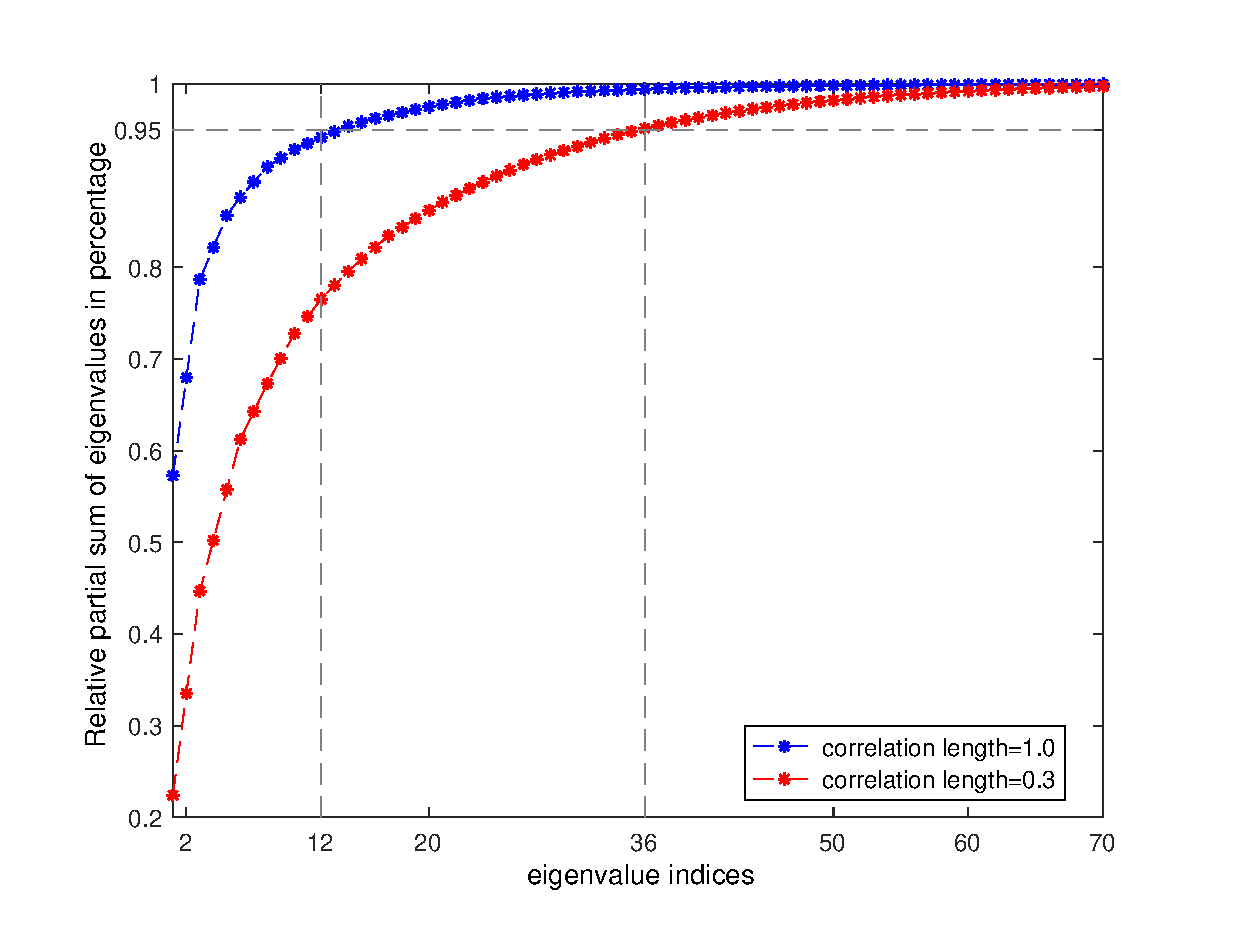
\includegraphics[width=0.6\textwidth,height=0.33\textheight]{plots/RelativeContribution_b1-03.eps}
 \caption{Relative partial sum of eigenvalues for exponential covariance kernel on a unit square domain.}
 \label{fig:eigenContribCompare}
\end{figure}
%----------------------------------------------------
Following the book by Ghanem and Spanos~\cite{ghanemSFEM1991}, a semi-analytical expression of the KLE is detailed for a Gaussian process.
Consider an exponential covariance function for a Gaussian stochastic process defined over a two-dimensional physical domain $\mathcal{D}(x,y)$ over the interval $[-a \ \ a] \times [-a \ \ a]$ ~\cite{ghanemSFEM1991}, %in \Cref{eq:exp2d}
\begin{equation}
C_{\alpha\alpha}({x}_1, {y}_1; {x}_2, {y}_2) = {\sigma}^2 e^{- | x_2 - x_1 | / b_1 \ - | y_2 - y_1 | / b_2},
\label{eq:exp2d}
\end{equation}
where $b_1$ and $b_2$ are the correlation lengths along $x$ and $y$ directions respectively and $\sigma^2$ denotes the variance of the underlying stochastic process.

Solving the integral given in \Cref{eq:cxx} for the covariance kernel given in \Cref{eq:exp2d}, the eigenvalues and eigenfunctions are obtained as~\cite{ghanemSFEM1991},
\begin{equation}\label{eq:eigval_2D}
  \lambda_n = \lambda^{x}_i  \otimes \lambda^{y}_i,
\end{equation}
  \begin{equation}
f_n(x, y) = g_i (x) \otimes h_i(y).
\label{eq:eigfn_2D}
\end{equation}
where $\otimes$ denotes the tensor product~\cite{smith2013uncertainty}. %(for example, see~\Cref{table:eigenTensor} in \Cref{apn:kle}).

\

The two-dimensional eigenfunctions $ \{ f_{n} \}_{n=1}^\infty$ and eigenvalues $ \{ \lambda_n \}_{n=1}^\infty$ are computed as the tensor product of the one-dimensional eigenfunctions $\{g_i(x), h_i(y)\}$ and eigenvalues  $\{\lambda^x_i, \lambda^y_i\}$ respectively~\cite{ghanemSFEM1991,ghanem1999stochastic}.
The analytical expressions for the one-dimensional eigenvalues and eigenfunctions for the exponential covariance kernel in~\Cref{eq:exp2d} are~\cite{ghanemSFEM1991,ghanem1999stochastic},
%which are computed , %The 1D eigenvalues and eigenfunctions
\begin{align}\label{eq:eigenVal}
\lambda^x_i &= {\sigma}^2  \frac{2b_1}{1 + b_1^2 {\omega_i}^2}, \nonumber \\
\lambda^y_i &= {\sigma}^2  \frac{2b_2}{1 + b_2^2 {\omega_i}^2},
\end{align}
\begin{equation}
 g_i(\textbf{\textit{x}}) = h_i(\textbf{\textit{x}}) =
\begin{cases}
& \frac{\cos({\omega}_i\textbf{\textit{x}})}{\sqrt{a + \frac{\sin(2{\omega}_i a)}{2 {\omega}_i}}}, \ \  \text{for} \  i \ \text{odd},   \nonumber \\
 & \frac{\sin({\omega}_i\textbf{\textit{x}})}{\sqrt{a - \frac{\sin(2{\omega}_i a)}{2 {\omega}_i}}}, \ \  \text{for} \  i \ \text{even},
 \end{cases}
\label{eq:eigenVec}
\end{equation}
where $\omega_i$'s are the solution of the following transcendental equations given by~\cite{ghanemSFEM1991,ghanem1999stochastic}
\begin{align}
 \frac{1}{b} - {\omega_i} \ \tan(\omega_i \  a) &= 0, \ \  \text{for} \  i \ \text{odd},  \nonumber \\
 {\omega_i} + \frac{1}{b} \ \tan(\omega_i \  a) &= 0, \ \  \text{for} \  i \ \text{even}.
 \label{eq:2D_omegas}
\end{align}
%Accordingly, the truncated KLE with $L$ modes can be written as
% \begin{equation}\label{eq:simplified_KLE}
% \alpha (\textbf{\textit{x}},  {\bxi}) =  \bar{\alpha}(\textbf{\textit{x}}) +  \sum^{L}_{n=1} \sqrt{{\lambda}_n} \ f_n(\textbf{\textit{x}}) {\xi_{n}}(\theta).
% \end{equation}
% for even-odd indices $i$, can simplified as
% \begin{equation}\label{eq:simplified_KLE}
% \alpha (\textbf{\textit{x}},  {\bxi}) =  \sum^{\infty}_{n=1} \left[ {\xi_{2n-1}} \sqrt{{\lambda}_{2n-1}} \ f_{2n-1}(x,y) + {\xi_{2n}} \sqrt{{\lambda}_{2n}} \ f_{2n}(x,y) \right]
% \end{equation}

The numerical implementation of KLE can be summarized in the following steps.
\begin{itemize}
\item Solve the transcendental equations given in \Cref{eq:2D_omegas} for $\omega_i$'s. \item Substitute $\omega_i$'s in \Cref{eq:eigenVal} and \eqref{eq:eigenVec} to compute the one-dimensional eigenvalues and eigenfunctions respectively. \item Using \Cref{eq:eigval_2D} and \eqref{eq:eigfn_2D} compute the two-dimensional eigenvalues $\{ \lambda_n \}_{n=1}^\infty$ and eigenfunction $ \{ f_{n} \}_{n=1}^\infty$ respectively and
\item using $\lambda_n$ and $f_n$ in \Cref{eq:truncatedKLE}, compute the KLE modes.
\end{itemize}
Note that the procedure presented above is for a two-dimensional physical domain. However, a similar procedure can be used for the cases with three-dimensional domains.
Refer to~\cite{desai2019scalable} for the further details on the implementation of KLE with the code snippets.

\subsection{Polynomial Chaos Expansion} \label{sec:PCE}
The KLE is a powerful tool that can be exploited in characterizing a stochastic process with a known covariance function.
%For instance, a random system operator with a well defined covariance kernel.
However,
%if the process does not have an explicitly defined covariance kernel,
the KLE cannot be used to represent a process with unknown covariance function.
%For example, the random system operator with a known covariance can be expanded using KLE. But, it cannot be used to represent the solution process, since its covariance function is unknown.
In such cases, the PCE can be utilized~\cite{ghanemSFEM1991,le2010spectral}.
%Also, for non-Gaussian stochastic processes, both the system parameters and solution process are represented using PCE.

%As per the Cameron-Martin theorem a second order stationary random process $\alpha(\textbf{\textit{x}}, \bxi(\theta))$ (as function of random event $\theta$) can be written as~\cite{cameron1947orthogonal,ghanemSFEM1991},
%\begin{align}
%\alpha(\textbf{\textit{x}}, \bxi(\theta)) & =  {\widehat{a}}_0{\psi}_0 +
%\sum^{\infty}_{i_{1}=1}{{\widehat{{ a}}}_{{\rm i_{1}}}\psi_1 {\rm
%(}{\xi }_{{\rm i_{1}}}\left(\theta \right){\rm )}} \nonumber\\
%&  +  \sum^{\infty}_{i_{1}=1}{\sum^{i_{1}}_{i_{2}=1}{{\widehat{{
%a}}}_{{\rm i_{1} i_{2}}}\psi_2 {\rm (}{\xi }_{\rm i_{1}}(\theta)},{\xi }_{\rm i_{2}}(\theta)}) \nonumber\\
%&  + \sum^{\infty}_{i_{1}=1}{\sum^{i_{1}}_{i_{2}=1}{\sum^{i_{2}}_{i_{3}=1}{{{\rm
%(}\widehat{{ a}}}_{{\rm i_{1} i_{2} i_{3}}}{\rm ) }\psi_3 {\rm (}{\xi
%}_{{\rm i_{1} }}(\theta)},{\xi }_{{\rm i_{2} }}(\theta),{\xi }_{{\rm i_{3} }}\left(\theta \right){\rm ) }}}
%\label{eq:cameron}
%\end{align}

%& & + \sum^{\infty}_{i_{1}=1}{\sum^{i_{1}}_{i_{2}=1}{\sum^{i_{2}}_{i_{3}=1}{\sum^{i_{3}}_{i_{4}=1}{{{\rm(}\widehat{{ a}}}_{{\rm i_{1} i_{2} i_{3} i_{4}}}{\rm ) }\psi_4 {\rm (}{\xi}_{{\rm i_{1} }}(\theta)},{\xi }_{{\rm i_{2} }}(\theta),{\xi }_{{\rm i_{3} }}(\theta),{\xi }_{{\rm i_{4} }} \left(\theta \right){\rm ) }}}} \nonumber\\& & + \ ... \ ... \ \infty.

%where ${\psi }_n (\bxi)$ denotes the polynomials chaoses of order $p$ in terms of $L$-dimensional independent random variables $ \bxi = ({\xi }_{ i_{1}}, {\xi }_{ i_{2}},{ \dots \dots , }{\xi }_{ i_{L}}) $ and $\widehat{a}$ represents unknown deterministic coefficients. For notational convenience eq.~\eqref{eq:cameron} can be rewritten as:

%There is an one-to-one relationship between the $\psi$'s and $\Psi$'s and also $\widehat{a}_j$'s and $a_j$'s in eq.~\eqref{eq:cameron} and ~\Cref{eq:pce}. Also, these polynomials are orthogonal in the statistical sense, i.e. their inner product with respect to probability measure is zero. Therefore, $\left< \Psi_i \ \Psi_j \right> = 0$ for $i \ne j$ and for other cases, it calculated as the statistical average~\cite{ghanemSFEM1991} as shown below,

A second order stochastic process $\alpha(\textbf{\textit{x}}, \bxi(\theta))$, i.e., a random process with finite variance %second moments
%as function of random event $\theta$
can be expanded using PCE as~\cite{ghanemSFEM1991},
\begin{equation}
\alpha(\textbf{\textit{x}}, \bxi(\theta)) = \sum^{\infty }_{j=0}{{ \widehat{\alpha_j}}(\textbf{\textit{x}}) \ {\Psi }_{
j}{\rm (}{\bxi(\theta)} {\rm )}},
\label{eq:pce}
\end{equation}
where ${\Psi }_j (\bxi(\theta))$ is a set of multidimensional orthogonal polynomials of the order $p_{\alpha}$ of $L$ independent random variables $\bxi = \{{\xi}_{1}, {\xi}_{2},{\dots,}{\xi}_{L} \} $ and ${\widehat{\alpha}}_j(\textbf{\textit{x}})$ represents the unknown deterministic coefficients.
Although the PCE is mainly founded on the independence assumption of the random variables, for some applications, there may exist significant dependence among the random variables. In such cases the Rosenblatt transformation~\cite{rosenblatt1952remarks}, commonly employed for mapping dependent to independent variables can be exploited (see the following articles for further details~\cite{soize2004physical,rahman2018polynomial}).

% \newpage
The polynomials ${\Psi }_j (\bxi)$ (note that the argument $\theta$ of $\bxi$ being dropped hereafter for notational simplicity) are orthogonal in a statistical sense, i.e., their inner product with respect to probability measure (PDF) is zero. Therefore, $\left< \Psi_i({\bxi}) , \Psi_j({\bxi}) \right> = 0$ for $i \ne j$ and for $i = j$, it can be computed as the statistical average as shown below~\cite{ghanemSFEM1991},
\begin{equation}
\left<  {\Psi }_{i}{\rm (}{\bxi} {\rm )} , {\Psi }_{j}{\rm (}{\bxi} {\rm )}\right> = \int {\Psi }_{i}{\rm (}{\bxi} {\rm )} {\Psi }_{j}{\rm (}{\bxi} {\rm )} \ {{\rm p}}({\bxi}) d\bxi,
\label{innerprod}
\end{equation}
where ${\rm p(.)}$ is the joint probability density function (PDF) of $\bxi$, obtained from the marginal PDF of ${\rm p_i(\bxi_i)}$ as: ${\rm p(\bxi)} = \prod_{i=1}^L {\rm p_i(\xi_i)}$.
%Note that, for the notational convenience $\theta$ is dropped from the preceding and forthcoming equations.

Theoretically, we need an infinite number of PCE terms to accurately approximate the output process.
%capture the entire spectrum. %as showed in \Cref{eq:pce}.
However, for the numerical approximation, the truncated PCE with $P_{\alpha}$ expansion terms can be used to obtain a sufficiently accurate representation of the output. Note that the higher order moments in the probability density function can be the measure of accuracy.
The truncated expansion given in ~\Cref{eq:truncatedpce} is shown to converge in the mean square sense~\cite{ghanemSFEM1991}:
%is shown to converge in the mean square sense~[WaadTh11, 96].
\begin{equation}
\alpha(\textbf{\textit{x}}, \bxi) = \sum^{P_{\alpha} }_{j=0}{{ \widehat{\alpha_j}}(\textbf{\textit{x}}) \ {\Psi }_{
j}{\rm (}{\bxi} {\rm )}},
\label{eq:truncatedpce}
\end{equation}
where the $P_{\alpha}$ is a function of the order of polynomials $p_{\alpha}$ and the number of random variables $L$ as given below~\cite{ghanemSFEM1991},
\begin{equation} \label{eq:np}
P_{\alpha} = \frac{(L+p_{\alpha})!}{L! \ p_{\alpha}!} - 1.
\end{equation}
The high-frequency random fluctuations in the stochastic process demand a large number of random variables and the strong nonlinear dependences of the solution process on the random system parameters necessitate the higher-order polynomials $p_{\alpha}$ in the PCE representation~\cite{ghanem1999ingredients,ghanem1999stochastic,huang2001convergence}.
Note that the order of polynomials can differ in the input and output PC expansions but the number of random variables $L$ should be the same~\cite{ghanemSFEM1991,le2010spectral,ghanem1999ingredients}.
In general, for better convergence, the output (solution) process is represented using higher order expansion than the inputs random process~\cite{ghanem1999ingredients,le2010spectral}. This is because the uncertainty in the output process may amplify as the input uncertainty undergoes nonlinear transformation through the model. This demands higher order expansion terms to capture the nonlinear and non-Gaussian effects. For further details on the convergence studies refer to the following articles~\cite{ghanem1999ingredients,ghanem1999stochastic,huang2001convergence}.
The implementational details and the associated code snippets of the PCE for a non-Gaussian stochastic process are presented in~\cite{desai2019scalable}.
%Appendices~\ref{apn:sto_pro} and \ref{apn:ssfem}.
%and the references therein
%For example, the PCE with second order polynomials chaos $(p=2)$ and four random variable $(L=4)$, we need 15-PCE terms $(n = 14)$. For clarity, a fully expanded form with 15-PCE terms is shown below.
%The PCE coefficients for the input lognormal stochastic process $l(\textbf{\textit{x}}, \bxi)$ denoting the underlying Gaussian process by $g(\textbf{\textit{x}}, \bxi)$ having a covariance function $C$ with a variance of $\sigma^{2}$ as given in~\Cref{eq:exp2d}. The KLE representation of $g(\textbf{\textit{x}}, \bxi)$ can be denote by \Cref{eq:simplified_KLE}~\cite{}. Therefore, the lognormal stochastic process $l(\textbf{\textit{x}}, \bxi)$ can be rewritten using KLE of underlying Gaussian as,
%\begin{equation}
%l(\textbf{\textit{x}}, \bxi) = \mathrm{exp} [ g(\textbf{\textit{x}}, \bxi) ].
%\end{equation}
%Consequently, using mathematical manipulations, the PCE of the lognormal stochastic process can be written as
%\begin{equation}\label{eq:pceLogNor}
%l(\textbf{\textit{x}}, \bxi)  = l_{0}(\textbf{\textit{x}}) \sum_{i=0}^{L} \frac{\left<\Psi_{i}(\boldsymbol\eta) \right>}{\left<\Psi_{i}^{2}(\bxi)\right>} \Psi_{i}(\bxi)
%\end{equation}
%where the quantity $\left<\Psi_{i}(\boldsymbol\eta) \right>$ is the expectation of the PC basis around the Gaussian coefficients. This can be evaluated analytically beforehand. The $l_{0}(\textbf{\textit{x}})$ is the mean of the lognormal stochastic process. The further details on the formulation and implementation of PCE for lognormal stochastic process can be found ~\cite{ghanem1999ingredients,ghanem1999stochastic,huang2001convergence}.


%Therefore, In either case, the number of PCE terms required to represent random system parameters and solution process dramatically increases~\cite{ghanemSFEM1991}.
%In the SSFEM literature, this issues is referred as the {\it{curse of dimensionality}}~\cite{ma2010adaptive,back2011stochastic,elman2011assessment,eldred2009comparison,stefanou2009stochastic,ganapathysubramanian2007sparse}.

%% The PCE for the log-normal stochastic process defined using underlying Gaussian random process with covariance function given above.... use this for thesis.

\section{Spectral Stochastic Finite Element Methods}\label{sec:SSFEM}

%Stochastic finite element method is emerged as a powerful tool which revolutionized the way modern engineering and scientific devices are designed. It helps us to account for the random heterogeneity in the system parameters and solution process and hence modeling of stochastic PDEs. In this article we'll focus on the spectral stochastic finite element method developed by Ghanem and Spanos~\cite{ghanemSFEM1991}.
%In this section, we first provide an overview the SSFEM followed by the formulation for intrusive SSFEM in \Cref{sec:IN}. The formulation of non-intrusive SSFEM using Smolyak sparse grid in given in \Cref{sec:NI}.
%Followed by performance comparison between these two approaches is discussed in \Cref{sec:inVni}.

%The next step is to use KLE and PCE to formulate the spectral stochastic finite element method.
In this section, we briefly describe the formulations of the intrusive and non-intrusive spectral stochastic finite element methods. For an elementary exposition of both the methodologies, we consider a linear elliptic stochastic PDE on a spatial domain $\mathcal{D}$ with the known boundary condition on $\partial \mathcal{D}$.
Consider a two-dimensional steady-state flow through random media with a spatially varying non-Gaussian diffusion coefficient $c_d$. The flow is modeled by a two-dimensional stochastic diffusion equation. This leads to a Poisson problem defined by a linear elliptic stochastic PDE %on a spatial domain $\mathcal{D}$ with a Dirichlet boundary condition
as defined below:
\begin{align}\label{eq:sspe}
-\nabla \ \cdotp \big( \ c_d(\textbf{\textit{x}},\theta) \ \ \nabla u(\textbf{\textit{x}}, \theta) \ \big) &= {F}(\textbf{\textit{x}}),     \ \ \  \ \ \ \   \mathcal{D}\times \Omega, \\
u(\textbf{\textit{x}}, \theta) &= 0,    \ \ \  \ \ \ \  \ \ \ \ \  \partial \mathcal{D}\times \Omega,
\end{align}
where $\nabla$ denotes the gradient which represents the differential operator with respect to the spatial variables $\textbf{\textit{x}}$, $u$ is the solution process,  $\theta$ is an element in the sample space $\Omega$ defined by the probability space ($\Omega, \mathcal{F}, \mathcal{P})$~\cite{billingsley2008probability}.
For the sake convenience, $F(\textbf{\textit{x}})$ is modeled as a deterministic source term. However, the methodology presented herein can be easily extended to stochastic source function $F(\textbf{\textit{x}},\theta)$.


To solve a partial differential equation, for instance \Cref{eq:sspe}, using finite element methods the PDE needs to be expressed in the variational form~\cite{le2010spectral,ciarlet2002finite}. To do so, first, the \Cref{eq:sspe} is multiplied by a test function $v$ and performing integration by parts we obtain~\cite{ciarlet2002finite}:
% This treatment results into %on to \Cref{eq:sspe_apn}
\begin{align}
  \int_{\mathcal{D}} c_d(\textbf{\textit{x}},\theta) \ \nabla u \ . \ \nabla v \ d\textbf{\textit{x}} = \int_{\mathcal{D}} F v \ d\textbf{\textit{x}} + \int_{\mathcal{\partial D}} \frac{\partial u}{\partial n} v \ ds,
\end{align}
where $u$ is called the trial function, $v$ is called the test function and ${\partial u}/{\partial n}$ is the derivative of $u$ in the outward normal direction at the boundary.
Note that $v$ vanishes where $u$ is known, i.e., on ${\mathcal{\partial D}}$.
Therefore, the resulting variation form can be further simplified as:
\begin{align}\label{eq:stoVar}
  \int_{\mathcal{D}} c_d(\textbf{\textit{x}},\theta) \ \nabla u \ . \ \nabla v \ d\textbf{\textit{x}} = \int_{\mathcal{D}} F v \ d\textbf{\textit{x}}.
\end{align}
Consider the diffusion coefficient $c_d(\textbf{\textit{x}},\theta)$, being modeled as a lognormal stochastic process $l(\textbf{\textit{x}},\theta)$ obtained by an exponential of a Gaussian process $g(\textbf{\textit{x}},\theta)$ having the mean $g_0(\textbf{\textit{x}})$, variance $\sigma^2$ and exponential covariance function $C_{gg}(x,y)$ in~\Cref{eq:exp2d}. For illustration, $c_d(\textbf{\textit{x}},\theta)$
is characterized by using two random variables with second order PCE. Therefore, PCE of the lognormal stochastic process can be expressed as~\cite{ghanemSFEM1991}. %(see \Cref{apn:lnp} for details).
\begin{align}\label{eq:cp2_logPCE3}
c_d(\textbf{\textit{x}},\theta) &= l_0(\textbf{\textit{x}}) \Big( g_0 + \xi_1(\theta) g_1(\textbf{\textit{x}}) + \xi_2(\theta) g_2(\textbf{\textit{x}}) + \big( \xi_1^2(\theta)-1 \big) \frac{g_1^2(\textbf{\textit{x}})}{2} \nonumber \\
&+  \big( \xi_1(\theta) \xi_2(\theta) \big) g_1(\textbf{\textit{x}}) g_2(\textbf{\textit{x}}) + \big( \xi_2^2(\theta)-1 \big) \frac{g_2^2(\textbf{\textit{x}})}{2} \Big),
\end{align}
where $\{ g_i(\textbf{\textit{x}}) \}_{i=1}^2$ are the scaled eigenfunctions of the covariance kernel $C_{gg}(x,y)$ and
$l_0(\textbf{\textit{x}}) = \mathrm{exp} \left[ g_0(\textbf{\textit{x}}) + \frac{1}{2} g_1^2(\textbf{\textit{x}}) + \frac{1}{2} g_2^2(\textbf{\textit{x}}) \right]$ is the mean of the lognormal process.

Consequently, \Cref{eq:stoVar} can be re-written as
\begin{align}\label{eq:stoVar2}
  & \int_{\mathcal{D}} l_0(\textbf{\textit{x}}) \Big( g_0 + \xi_1(\theta) g_1(\textbf{\textit{x}}) + \xi_2(\theta) g_2(\textbf{\textit{x}}) + \big(\xi_1^2(\theta)-1 \big) \frac{g_1^2(\textbf{\textit{x}})}{2} \nonumber \\
  &+  \big( \xi_1(\theta) \xi_2(\theta) \big) g_1(\textbf{\textit{x}}) g_2(\textbf{\textit{x}}) + \big( \xi_2^2(\theta)-1 \big) \frac{g_2^2(\textbf{\textit{x}})}{2} \Big) \ \nabla u \ . \ \nabla v \ d\textbf{\textit{x}} = \int_{\mathcal{D}} F v \ d\textbf{\textit{x}}.
\end{align}

The finite element discretization with $N$ nodes in the spatial domain leads to a system of linear equations with random coefficients $\theta$ denotes stochasticity~\cite{ghanemSFEM1991}
\begin{equation}\label{eq:dFEM}
{\mathrm{\bf{A}(\theta) \bf{u}(\theta) = \bf{f}}},
\end{equation}
where ${\mathrm{\bf{A}}(\theta)}$ is the random or stochastic system matrix, $ \bf{u}(\theta)$ is the stochastic response vector and $\bf{f}$ is the deterministic source vector. In the deterministic setting the above system of equations can be solved for the mean values of the stochastic parameters. For example, the Gaussian process characterized by using $g_0 = 0$, $\sigma=0.3$ and the exponential covariance function given in~\Cref{eq:exp2d} with $b_1=b_2=b=1$. Therefore, $c_d$ can be expanded as~\cite{ghanemSFEM1991} (for simplification using $L\rightarrow \infty$
, refer to~\cite{ghanem1999ingredients,ghanem1999nonlinear} for details). %\Cref{apn:lnp}
\begin{align}\label{eq:logPCE}
c_d(\textbf{\textit{x}},\theta) &= l_0 = \mathrm{exp} \left[  0 + \frac{1}{2}{0.3}^2 \right] = 1.05.
\end{align}

Consider a unit square domain discretized using unstructured finite element mesh with $600$ nodes and $1200$ elements as shown in \Cref{fig:mean_SSFEM}. The numerical simulations are performed using
the unit source term.
The solution field for the mean value of stochastic parameter is shown in~\Cref{fig:mean_SSFEM}.
The corresponding FEniCS based python code snippet is shown in Listing ~\cite{desai2019scalable}. %\ref{list:det_fem}.

%-------------------Abhi commented-------------
\begin{figure}[htbp]
\centering
 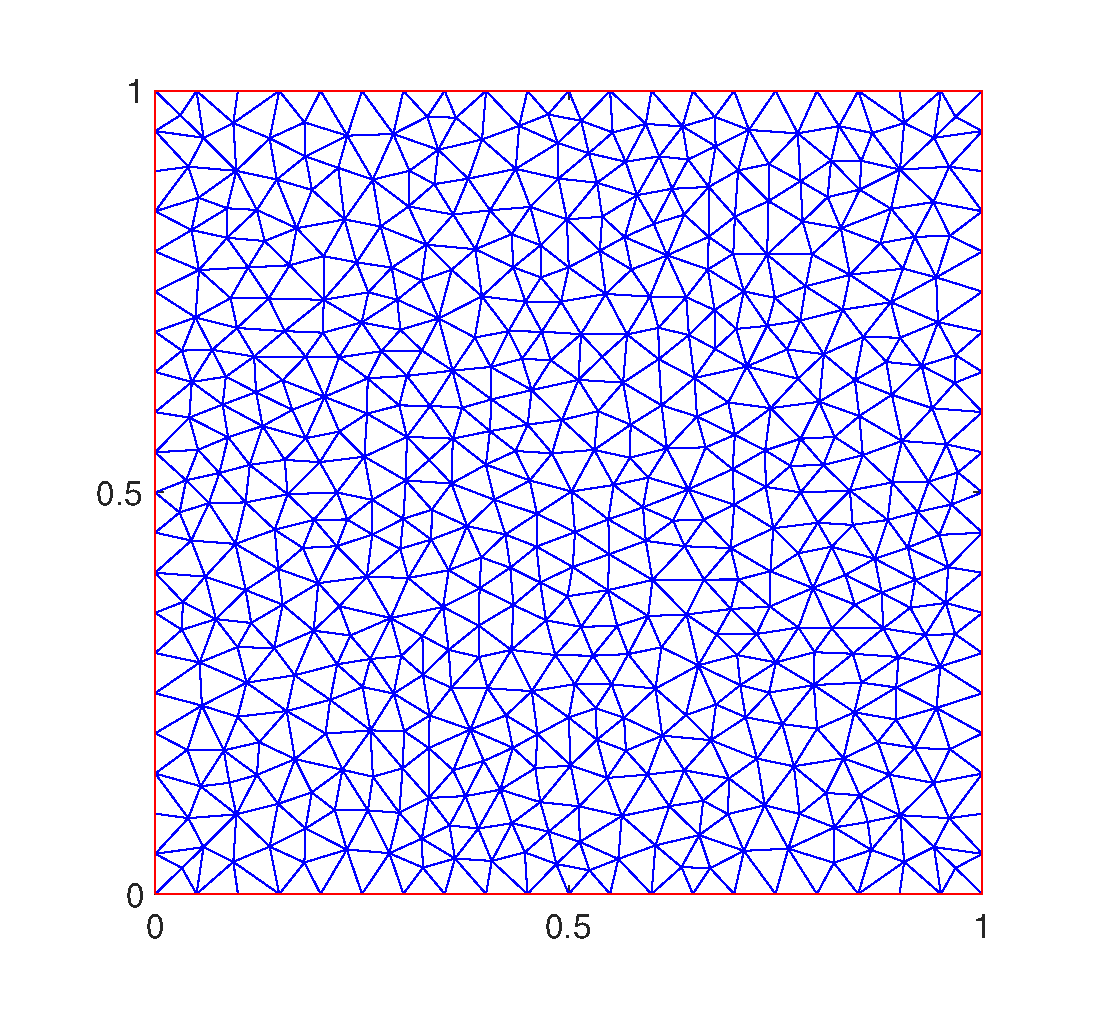
\includegraphics[width=0.42\textwidth,height=0.27\textheight]{plots/apn_mesh.eps}
 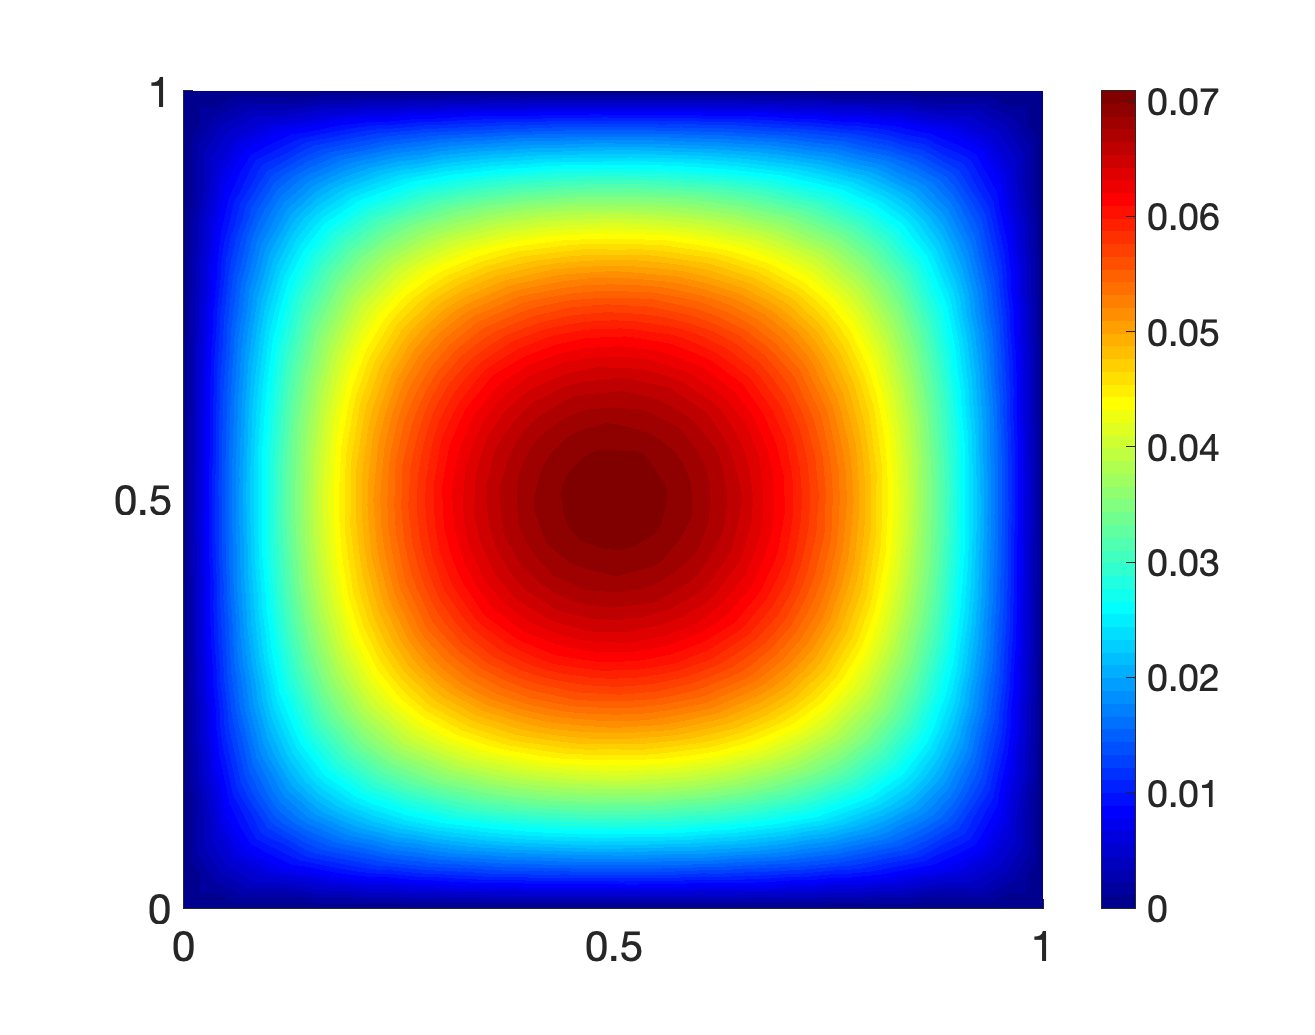
\includegraphics[width=0.5\textwidth,height=0.27\textheight]{plots/apn_mean_solution.eps}
 \caption{Finite element mesh and the solution field at the mean value of stochastic system parameters.}
 \label{fig:mean_SSFEM}
\end{figure}
%------------------------------------------

Assuming that the input data contains sufficient statistical information, we can represent the random system matrix and the stochastic solution process using the PCE as~\cite{ghanemSFEM1991}:
\begin{align}
{\mathrm{\bf{A}(\theta)}} =  \sum^{P_{\textsc{a}}}_{i=0} {\hat{{\mathrm{\bf{A}}}}_i} \ {\Psi_i(\bxi)},  \ \ \ \ \  {\mathrm{\bf{\tilde{u}}(\theta)}} =  \sum^{P_{u}}_{j=0} {\mathrm{\hat{\bf{u}}}_j}  \ {\Psi_j(\bxi)},
\label{eq:pceinout}
\end{align}
where the $\hat{{\mathrm{\bf{A}}}}_i$'s are the PCE coefficients of the random system matrix, $\hat{{\bf{u}}}_j$'s are the PCE coefficients of the solution process and $\Psi$'s are the multidimensional polynomials obtained as a function of $L$ random variables ${\bxi} = \{ \xi_{1}, \xi_{2}, \dots, \xi_{L} \}$.
$P_{\textsc{a}}$ and $P_{u}$ are the numbers of PCE terms required to characterize the stochastic system matrix and the stochastic response vector respectively~\cite{ghanemSFEM1991}.
The number of PCE terms $P_{\alpha}$ is a function of the order of polynomials $p_{\alpha}$ and the number of random variables $L$, which can be computed using~\Cref{eq:np}~\cite{ghanemSFEM1991} and the subscript $\alpha$ represents $\textsc{a}$ or $u$. In this study the input, namely the diffusion coefficient of the Poisson PDE is modeled by a lognormal process obtained by the exponential of a Gaussian process.  For further details on the PCE of the lognormal process and KLE of the underlying Gaussian process refer to~\cite{desai2019scalable}.

%The $P_{\alpha}$'s for input and output processes are computed using \Cref{eq:np}~\cite{ghanemSFEM1991}.
% \begin{equation} \label{eq:np}
% P_{\alpha} = \frac{(L+p_{\alpha})!}{L! \ p_{\alpha}!} - 1.
% \end{equation}
% The  $P_{\textsc{a}}$ and $P_{u}$ are computed from \Cref{eq:np} using $L$ random variables with $p_{\textsc{a}}$ and $p_{u}$ as the order of polynomials in the PCE of ${\mathrm{\bf{A}(\theta)}} $ and ${\mathrm{\bf{u}(\theta)}}$ respectively.


%The required number of PCE terms for random inputs and random output can be obtained from the following equations respectively.
%\begin{equation}
%P_{\textsc{a}} = \frac{(L+p_{\textsc{a}})!} {L! \ p_{\textsc{a}}!}, \ \ \ \ \   P_{u} = \frac{(L+p_{u})!} {L! \ p_{u}!}.
%\end{equation}
%Where $L$ represents the number of random variables (also referred as stochastic dimensions) used to characterize the input random process and the solution process. The $p_{\textsc{a}}$ and $p_{u}$ are the order of polynomials used in PC expansion for random input and the solution process respectively. Therefore, the number of PCE terms required to represent stochastic input and output is highly dependent on both stochastic dimensions $L$ and order or expansions $p$.

% \Cref{apn:sto_pro} details the PCE of the lognormal process and KLE of the underlying Gaussian process.
%The PCE coefficients for the input stochastic process with a known covariance function, i.e., in this case, ${\hat{{\mathrm{\bf{A}}}}_i}$   are obtained using KLE (refer to~\Cref{apn:kle} for more details)~\cite{ghanemSFEM1991,ghanem1996numerical,pellissetti2000iterative}.
In the SSFEM approaches, the primary goal is to compute the PCE coefficients of the solution process ${\hat{\bf{u}}}_{j}$.
Based on the approach utilized to compute ${\hat{\bf{u}}}_{j}$, the solution methodologies for SSFEM are generally classified into (a) intrusive (sampling-free) approach also referred to as the stochastic Galerkin (SG) approach~\cite{ghanemSFEM1991,ghanem1996numerical,pellissetti2000iterative,sarkarIJNME2009,ullmann2012efficient} and (b) non-intrusive (sampling-based) approaches such as non-intrusive spectral projection (NISP)~\cite{le2010spectral,reagana2003uncertainty,hosder2006non,eldred2009comparison,desai2010analysis} or stochastic collocation (SC) approach~\cite{babuvska2007stochastic,xiu2007efficient,ganapathysubramanian2007sparse,nobile2008sparse}.
Note that, in this paper, we have focused on the SG and the NISP approach based on the sparse grid quadrature.

In the SG (intrusive) approach, the PCE for the random system parameters and the solution process, for example as given in~\Cref{eq:pceinout} are substituted into the governing equation (for example \Cref{eq:dFEM}).
In SG framework the strategy is to project the residual onto a finite-dimensional space spanned by appropriate orthogonal basis functions with respect to probability density $\mathrm{p}(\bxi)$. Thus we seek the approximate solution as~\cite{smith2013uncertainty}
\begin{align}\label{eq:sg_int}
 0 &= \Big\langle  {\mathrm{\bf{A}(\theta) \bf{u}(\theta) - \bf{f}}} \ , \Psi_k(\bxi) \Big\rangle, \ \ k=0,1,\dots,P_u,  \\ \nonumber
  &= \int_{\mathscr{D}} \Big[ \sum^{P_{\textsc{a}}}_{i=0} {\hat{{\mathrm{\bf{A}}}}_i} \ {\Psi_i(\bxi)}   \sum^{P_{u}}_{j=0} {\mathrm{\hat{\bf{u}}}_j}  \ {\Psi_j(\bxi)} - {\bf{f}} \Big] \Psi_k(\bxi) \mathrm{p}(\bxi) d\bxi, \ \ k=0,1,\dots,P_u.
\end{align}
\Cref{eq:sg_int} can also be approximately solved using the quadrature rule with quadrature points $q_n$ and weights $w_n$ as
\begin{align} \label{eq:sg_int2}
  \sum_{n=1}^{N} \Big[ \sum^{P_{\textsc{a}}}_{i=0} {\hat{{\mathrm{\bf{A}}}}_i} \ {\Psi_i(q_n)}   \sum^{P_{u}}_{j=0} {\mathrm{\hat{\bf{u}}}_j}  \ {\Psi_j(q_n)} - {\bf{f}} \Big] \Psi_k(q_n) \ \mathrm{p}(q_n) w_n = 0, \ \ k=0,1,\dots,P_u.
\end{align}

In the NISP framework (also referred as pseudo-spectral approach) the PCE  coefficients of solution process are obtained by performing Galerkin projection on the PCE of the solution process given in \Cref{eq:pceinout}. The orthogonality properties of PCE basis functions are utilized to compute the expansion coefficients of the solution process~\cite{ghanemSFEM1991,le2010spectral} as,
\begin{equation}
{\mathrm{\hat{\bf{u}}}_k} = \frac{1} {\left<{\Psi_k^2({\pmb{\xi}})}  \right>} \sum_{n=1}^{N} {\mathrm{\bf{u}}(q_n)} \Psi_k(q_n) \ \mathrm{p}(q_n) w_n, \ \ k=0,1,\dots,P_u.
\label{eq:NISPpce_framework}
\end{equation}
The NISP approach is simple to implement; however, for the cases with a large number of random variables (which is the primary focus of this paper) the number of quadrature points required to solve the above integral increases significantly~\cite{smith2013uncertainty,hosder2006non,eldred2009comparison,eldred2009recent}.

In the framework of collocation approach, $M$ collocation points are generated from the parameter space, and then enforce
\begin{equation}
  \mathrm{\bf{u}}(q_m) = \mathrm{\tilde{\bf{u}}}(q_m), \ \ m=1,\dots,M
\end{equation}
to compute $\mathrm{\hat{\bf{u}}}_j$. For a general basis function $\phi_k$, performing above steps yields the following system~\cite{smith2013uncertainty}

\begin{align}
{\begin{bmatrix}
      \phi_{0}(q_1) & \dots  &  \phi_{P_u}(q_1)
\\[0.3em]
      \vdots  & \ddots &  \vdots
\\[0.3em]
      \phi_{0}(q_M) & \dots  &  \phi_{P_u}(q_M)
\\[0.3em]
\end{bmatrix}}
\begin{Bmatrix}
    \mathrm{\hat{\bf{u}}}_0
\\[0.3em]
   \vdots
\\[0.3em]
    \mathrm{\hat{\bf{u}}}_{P_u}
 \\[0.3em]
\end{Bmatrix}  =
\begin{Bmatrix}
      \mathrm{\bf{u}}(q_1)
\\[0.3em]
      \vdots
 \\[0.3em]
      \mathrm{\bf{u}}(q_M)
\end{Bmatrix}.
\label{eq:coll_frame}
\end{align}
Similar to the NISP approach, the SC approach is also straightforward to formulate. However, for a large number of random variables, the number and choice of collocation points as well as the choice of basis function become critical~\cite{smith2013uncertainty}.
Note that the computational efforts required for the collocation approach is essentially equivalent to that of NISP approach when the number of collocation points $M$ equal to quadrature points $N$.

The accuracy of intrusive (SG) approach is optimal in $\mathrm{L}^2$ sense. Therefore, the SG approach can be computationally efficient over NISP or SC methods~\cite{smith2013uncertainty}. However, SG approach involves substantial modification of a deterministic simulation code~\cite{smith2013uncertainty}.
%the SG approach is primarily criticized for the requirement of intrusive adjustments which necessitates the new simulation code~\cite{smith2013uncertainty}. Also, as pointed out in~\cite{smith2013uncertainty}, the SG approach can be used only for PDF with associated orthogonal polynomials and it is relies on the assumption that the random variables are independent. However, we would like to point out that the Rosenblatt transformation~\cite{rosenblatt1952remarks} can be employed to overcome the dependence issue (see following articles for details~\cite{soize2004physical,rahman2018polynomial}).
Note that, later in this paper, we demonstrate that the requirement of
modification of a deterministic simulation code due to intrusive adjustments in the SG approach can be alleviated by employing general purpose deterministic FEM packages (e.g. FEniCS~\cite{fenics/dolfin17}).

On the other hand, the SC approach does not encounter orthogonality and dependence requirement issues observed in SG approach. The SC approach can be applied to general parameter distribution (see~\cite{eldred2009comparison,smith2013uncertainty} for more details). However, the SC is a sampling-based approach and the number of required samples grow with the order and the number of random variables. Similarly, in the NISP approach the number of quadrature points grow with the order and number of random variables.
Note that, the SC approach is not implemented in this paper, instead we use NISP approach based on the sparse grid quadrature.
For more details on the SC approach and its comparison with NISP and SG approaches the author refer to the numerous articles available in the literature~\cite{babuvska2007stochastic,xiu2007efficient,ganapathysubramanian2007sparse,nobile2008sparse,eldred2009comparison,smith2013uncertainty}.


The rest of the paper is organized as follows: \Cref{sec:IN} outlines the formulation of intrusive SSFEM (SG).
This is followed by the formulation of non-intrusive approach, specifically, the NISP with Smolyak sparse grid quadrature in~\Cref{sec:NI}.
In~\Cref{sec:inVni} the performance comparison of the intrusive SSFEM with the non-intrusive SSFEM is conducted using a Poisson equation having a non-Gaussian diffusion coefficient, modeled by a lognormal process.
%Finally, in~\Cref{cp1:sec_mtdSSFEM}, an overview of the solution methods for intrusive SSFEM system is discussed.

%{\it{NISP is selected over SC approach mainly because, we wan't to compare the behaviour of each of the PCE coefficients of the solution process for intrusive and non-intrusive}}.




\subsection{Intrusive SSFEM} \label{sec:IN}
In the intrusive SSFEM, the PCE of the system matrix with random coefficients ${\mathrm{\bf{A}(\theta)}}$ and the solution process ${\mathrm{\bf{u}(\theta)}}$, presented in \Cref{eq:pceinout} are directly substituted into the finite element discretization of stochastic PDE given in \Cref{eq:dFEM} leading to~\cite{ghanemSFEM1991}
%(\textcolor{blue}{need to verify this equation from Ghanem's book)
\begin{equation}
\epsilon = \sum^{P_{\textsc{a}}}_{i=0} {\hat{{\mathrm{\bf{A}}}}_i} {\Psi_i({\pmb{\xi}})}
\ \sum^{P_{u}}_{j=0} {\mathrm{\hat{\bf{u}}}_j} {\Psi_j({\pmb{\xi}})} - {\mathrm{\bf{f}}} \neq 0,
\label{eq:skuf}
\end{equation}
where $\epsilon$ is the random residual.

Performing Galerkin projection, i.e., multiplying both sides of the \Cref{eq:skuf} by ${\Psi_k({\pmb{\xi}})}$ with $k = 0,..,P_{u}$ and taking expectation both sides results in the following system of coupled equations~\cite{ghanemSFEM1991},
\begin{equation}
  \left< \epsilon , {\Psi_k({\pmb{\xi}})} \right> = 0 \ , \ \ \ \ \   k = 0,1,\dots,P_{u}
\end{equation}
\begin{equation}
\sum^{P_{u}}_{j=0} \sum^{P_{\textsc{a}}}_{i=0} \left< {\Psi_i({\pmb{\xi}})} {\Psi_j({\pmb{\xi}})} {\Psi_k({\pmb{\xi}})} \right>  {\hat{{\mathrm{\bf{A}}}}_i}  {\mathrm{\hat{\bf{u}}}_j}    =  \left< {\mathrm{\bf{f}}} \ {\Psi_k({\pmb{\xi}})} \right> , \ \ k = 0,1,\dots,P_{u}.
\label{eq:gpkuf}
\end{equation}
For notational convenience, we rewrite \Cref{eq:gpkuf} using $\left< {\Psi_i({\pmb{\xi}})} {\Psi_j({\pmb{\xi}})} {\Psi_k({\pmb{\xi}})} \right> = \mathbfcal{C}_{ijk}$  and $ \left< {\mathrm{\bf{f}}} \ {\Psi_k({\pmb{\xi}})} \right> = f_{k}$ leading to
\begin{equation}
\sum^{P_{u}}_{j=0} \sum^{P_{\textsc{a}}}_{i=0}  \mathbfcal{C}_{ijk} {\hat{{\mathrm{\bf{A}}}}_i} \ {\mathrm{\hat{\bf{u}}}_k}   =  f_{k} \ , \ \ \ \ \   k = 0,1,\dots,P_{u}.
\label{eq:cijkkuf}
\end{equation}
For concise representation, the following notation is used,
\begin{equation}\label{eq:sFEMatrix}
A_{jk} =  \sum^{P_{\textsc{a}}}_{i=0}  \mathbfcal{C}_{ijk} {\hat{{\mathrm{\bf{A}}}}_i},
\end{equation}
%%\ , \ \ \ \ \ u_{k} = ({\mathrm{\hat{\bf{u}}}_0}, {\mathrm{\hat{\bf{u}}}_1}, \dots, {\mathrm{\hat{\bf{u}}}_{P_{u}}})^{\textsc{t}}.
Thus, \Cref{eq:cijkkuf} can be further simplified as,
\begin{equation}
\sum^{P_{u}}_{j=0}  A_{jk}  \ {\mathrm{\hat{\bf{u}}}_k}    = f_k \ ,  \ \ \ \ \   k = 0,1,\dots,P_{u}.
\label{eq:Gakuf}
\end{equation}
%The expanded form of Eq.\ref{Gakuf}
%\begin{equation}\label{globAsem}
%{\begin{bmatrix}
%      [A_{0,0}] & [A_{0,1}] & \dots  &  [A_{0,P_{u}}]
%\\[0.3em]
%     [A_{1,0}] & [A_{1,1}] & \dots  &  [A_{1,P_{u}}]
%\\[0.3em]
%      \vdots   & \ddots & \vdots \ \  &  \vdots
%\\[0.3em]
%     [A_{P_{u},0}] & [A_{P_{u},1}] & \dots  &  [A_{P_{u},P_{u}}]
%\end{bmatrix}}
%\begin{Bmatrix}
%      {\mathrm{\hat{\bf{u}}}_0}
%\\[0.3em]
%      {\mathrm{\hat{\bf{u}}}_1}
% \\[0.3em]
%        \vdots
% \\[0.3em]
%       {\mathrm{\hat{\bf{u}}}_{P_{u}}}
% \\[0.3em]
%\end{Bmatrix}  =
%\begin{Bmatrix}
%      f_0
%\\[0.3em]
%      f_1
%\\[0.3em]
%       \vdots
% \\[0.3em]
%      f_{P_{u}}
%\end{Bmatrix},
%\end{equation}
Equivalently \Cref{eq:Gakuf} can be written as,
\begin{equation}\label{eq:sFEM}
\mathcal{[A] \{U\} = \{F\}},
\end{equation}
%Solution of \Cref{eq:sFEM} gives the PCE coefficients of the solution process $\{ \mathcal{U} \}$.
where $\mathcal{A}$ in \Cref{eq:sFEM} is the system matrix,
$\mathcal{U}$ is the vector of PCE coefficients of the solution process and
$\mathcal{F}$ is the corresponding right hand side vector arising in the setting of intrusive SSFEM. \Cref{eq:sFEM} can be expanded as
\begin{align}
{\begin{bmatrix}
      A_{0,0} & A_{0,1} & \dots  &  A_{0,P_u}
\\[0.3em]
      A_{1,0} & A_{1,1} & \dots  &  A_{1,P_u}
\\[0.3em]
      \vdots  & \vdots  & \ddots &  \vdots
\\[0.3em]
     A_{P_u,0} & A_{P_u,1} & \dots  &  A_{P_u,P_u}
\end{bmatrix}}
\begin{Bmatrix}
    \mathrm{\hat{\bf{u}}}_0
\\[0.3em]
    \mathrm{\hat{\bf{u}}}_1
 \\[0.3em]
    \vdots
 \\[0.3em]
    \mathrm{\hat{\bf{u}}}_{P_u}
 \\[0.3em]
\end{Bmatrix}  =
\begin{Bmatrix}
      f_0
\\[0.3em]
      f_1
\\[0.3em]
      \vdots
 \\[0.3em]
      f_{P_u}
\end{Bmatrix}.
\label{eq:sFEM_expnd}
\end{align}
The solution of the above coupled linear system yields the PCE coefficients of the solution process. These PCE coefficients can be used to obtain the mean, variance, higher order statistics and PDF of the solution process~\cite{ghanemSFEM1991}.
% \begin{align}
% \mu_{\mathrm{\bf{u}}} = \sum_{i=0}^{P_u}  \< \Psi_i \> \mathrm{\hat{\bf{u}}}_i
% \end{align}

The size of the system matrix $\mathcal{A}$ is $(N\times P_{u} ,  N\times P_{u})$, where $N$ is the number of degree-of-freedom related to the finite element mesh resolution and $P_{u}$ is the number of PCE terms used in the representation of the solution process.
Note that, $P_{u}$ is a function of stochastic dimension $L$ and order $p_{u}$ of the PCE.
%For a fixed mesh resolution, as the stochastic dimension and/or polynomial order increases, the $P_{u}$ grows drastically. Hence, the size of the stochastic finite element matrix grows quickly and becomes the bottleneck of the method.
%In the current study the primary attention is given to the effect of increasing number of random variables $L$ while keeping other two parameters constant.
%Moreover, the assembly of stochastic finite element matrix requires intruding into the governing PDE thus demands development of new solver. To alleviate this issue, the author proposes an efficient stochastic matrix assembly procedure outlined in \Cref{alg:smap}.
From \Cref{eq:sFEMatrix} and \eqref{eq:Gakuf} it can be noted that, each block of the system matrix $\mathcal{A}$ is denoted by $A_{jk}$ (a sub matrix of size $(N \times N))$ and it can be computed from the set of deterministic finite element matrices ${\hat{{\mathrm{\bf{A}}}}_i}$. %Therefore, with minor changes in existing deterministic FE assembler, one can assemble the stochastic finite element assembly matrix.
In this paper, the system matrix assembly procedure, i.e., implementation of~\Cref{eq:sFEMatrix} is performed by
%the stochastic finite element matrix assembly procedure is performed by %procedure outline in \Cref{alg:smap}
employing deterministic finite element assembly routines imported from the {\it{FEniCS}} general purpose FEM package~\cite{logg2012FEniCS,aloggs2013puffin}.
%Alternatively, the proposed stochastic assembly procedure can be performed while directly using more advanced FEniCS/dolfin assembly routines~\cite{}.
%to demonstrate the ease of implementation of intrusive SSFEM.


%%%***************************************************************************************
%\alglanguage{pseudocode}
%\begin{algorithm}
%\caption{: \textcolor{blue}{intrusive system matrix Assembly Procedure (SFEM-AP)}}
%\label{alg:smap}
%\begin{algorithmic}[1]
%\State {\bf{Input} :}  non-zero : $ijk$ and $C_{ijk}$
%\For{$ {i = 0, 1, 2, ..., P_{\textsc{a}}}   $}
%\State Call Modified \textcolor{red}{Deterministic Matrix Assembly} ( ${\hat{{\mathrm{\bf{[A]}}}}_i}$ )
%\For{$ {j = 0, 1, 2, ..., P_{u}}  $}
%\For{$ {k = 0, 1, 2, ..., P_{u}}  $}
%\If{$ i, j, k == nonZero(ijk) $}
%\State \textcolor{red}{Stochastic Matrix Assembly} ( $\mathcal{[A]}_{j,k} \ += C_{ijk}*{\hat{{\mathrm{\bf{[A]}}}}_i}$ )
%\EndIf
%\EndFor
%\EndFor
%\EndFor
%\State {\bf{Output} :}  $\mathcal{[A]}$
%\end{algorithmic}
%\end{algorithm}

%The implementation of \Cref{alg:smap} requires to follow the following steps. First calculate and store the non-zero moments of multidimensional polynomials $C_{ijk}$'s and their respective indices $ijk$. This re-quire computation of multidimensional inner products which are obtained using one-dimensional moments~\cite{le2010spectral} employing the routines adapted from UQ Toolkit~\cite{debusschere2013uqtk}.
%Next, for each of the input PCE index $i$ call the deterministic assembly procedure slightly modified to accommodate the respective input PCE coefficients and temporarily store the assembled matrix ${\hat{{\mathrm{\bf{[A]}}}}_i}$.
%For all the output PCE indices $j,k$, those matches with the stored non-zero $ijk$ indices, multiply assembled deterministic matrix with respective $C_{ijk}$ and store it in respective $j,k$ position of stochastic matrix $\mathcal{[A]}_{j,k}$.

%The stochastic assembly procedure outlined here is designed to reduce the number of call to deterministic assembly routines and also to reduce required memory by recursively using the available memory. Hence optimizing both memory and floating point operation count. Also the computational burden is reduced by invoking the calculations for a non-zero ${ijk}$ indices only.


The intrusive system matrix $\mathcal{A}$ has the two-levels of sparsity (block-sparse structure), for example, see in \Cref{fig:SFEM1} and \ref{fig:SFEM2}~\cite{ghanem1996numerical,ghanem1999stochastic,pellissetti2000iterative}. The first-level of sparsity is coming from the deterministic finite element matrices, ${\hat{{\mathrm{\bf{A}}}}_i}$, which are sparse and the second-level of sparsity is due to the stochastic aspects of the problem arising from a few non-zero $\mathbfcal{C}_{ijk}$ terms.
The matrices in \Cref{fig:SFEM1} and \ref{fig:SFEM2} are assembled for the stochastic diffusion equation with a lognormal diffusion coefficient represented using the underlying Gaussian stochastic process (refer to ~\cite{desai2019scalable} for further details).

%-------Abhi commented--------------
\begin{figure}[htbp]
\centering
 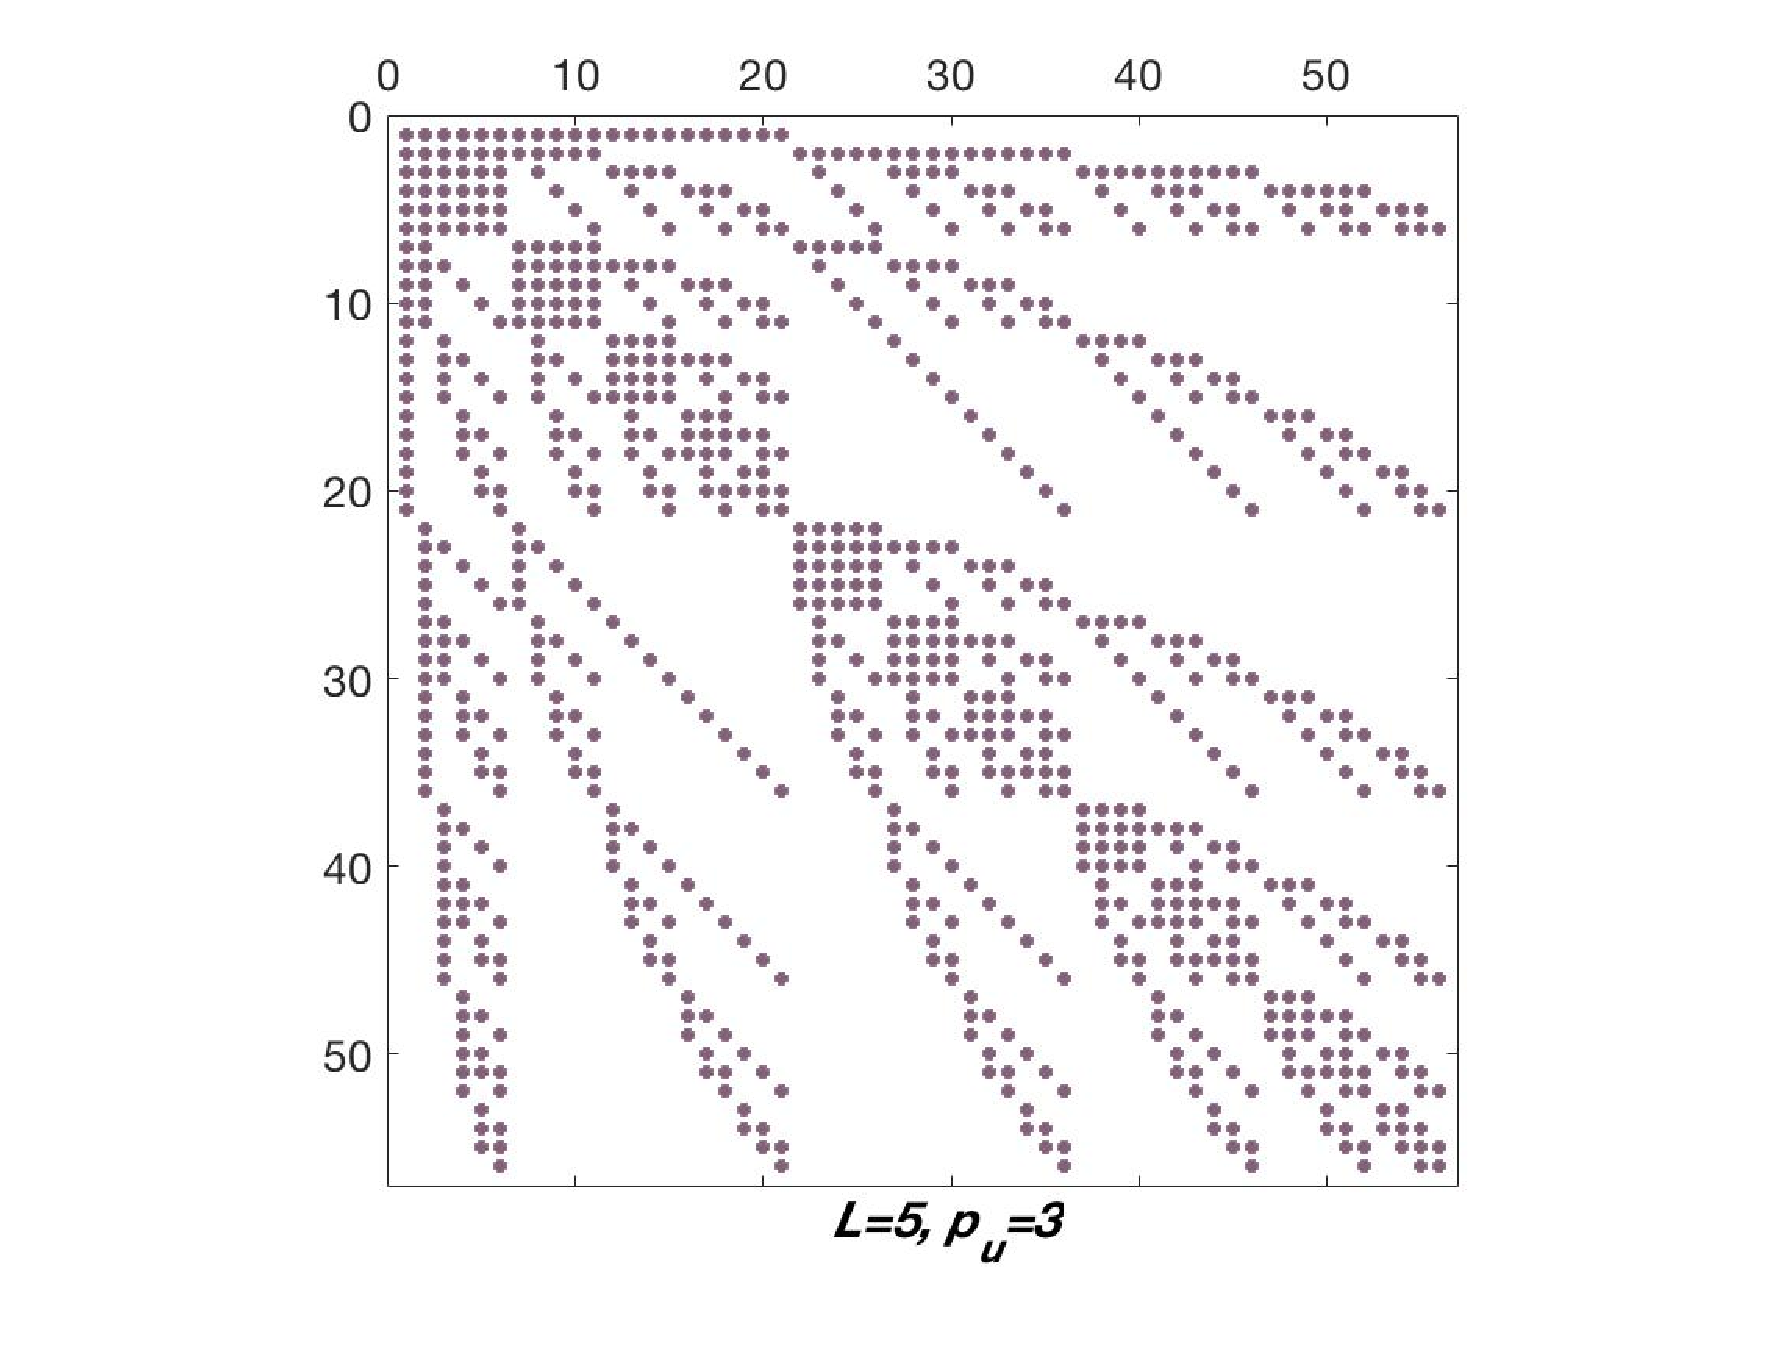
\includegraphics[width=0.32\textwidth,height=0.17\textheight]{plots/L5p3_n30.eps}
 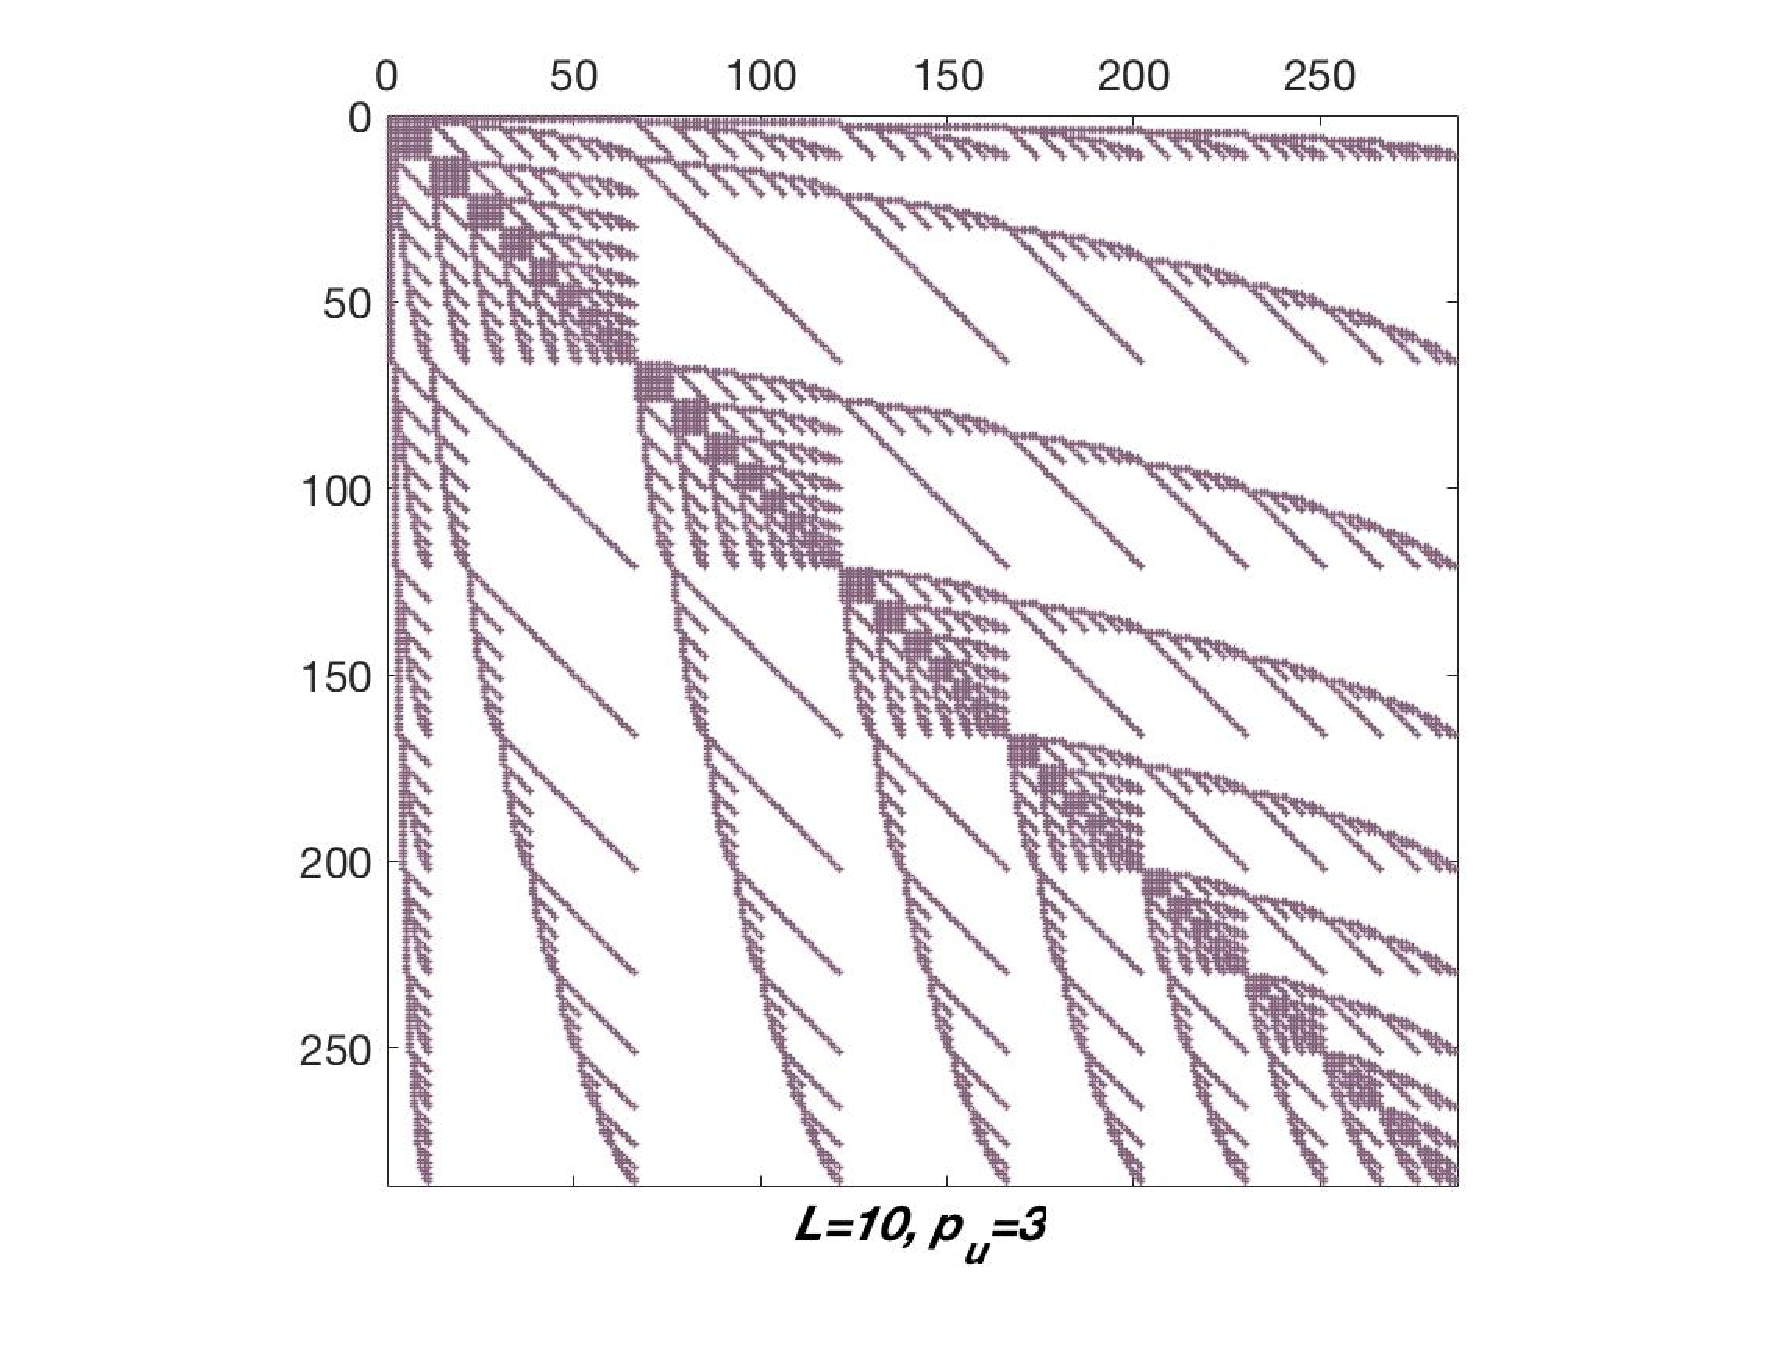
\includegraphics[width=0.32\textwidth,height=0.17\textheight]{plots/L10p3_n30.eps}
 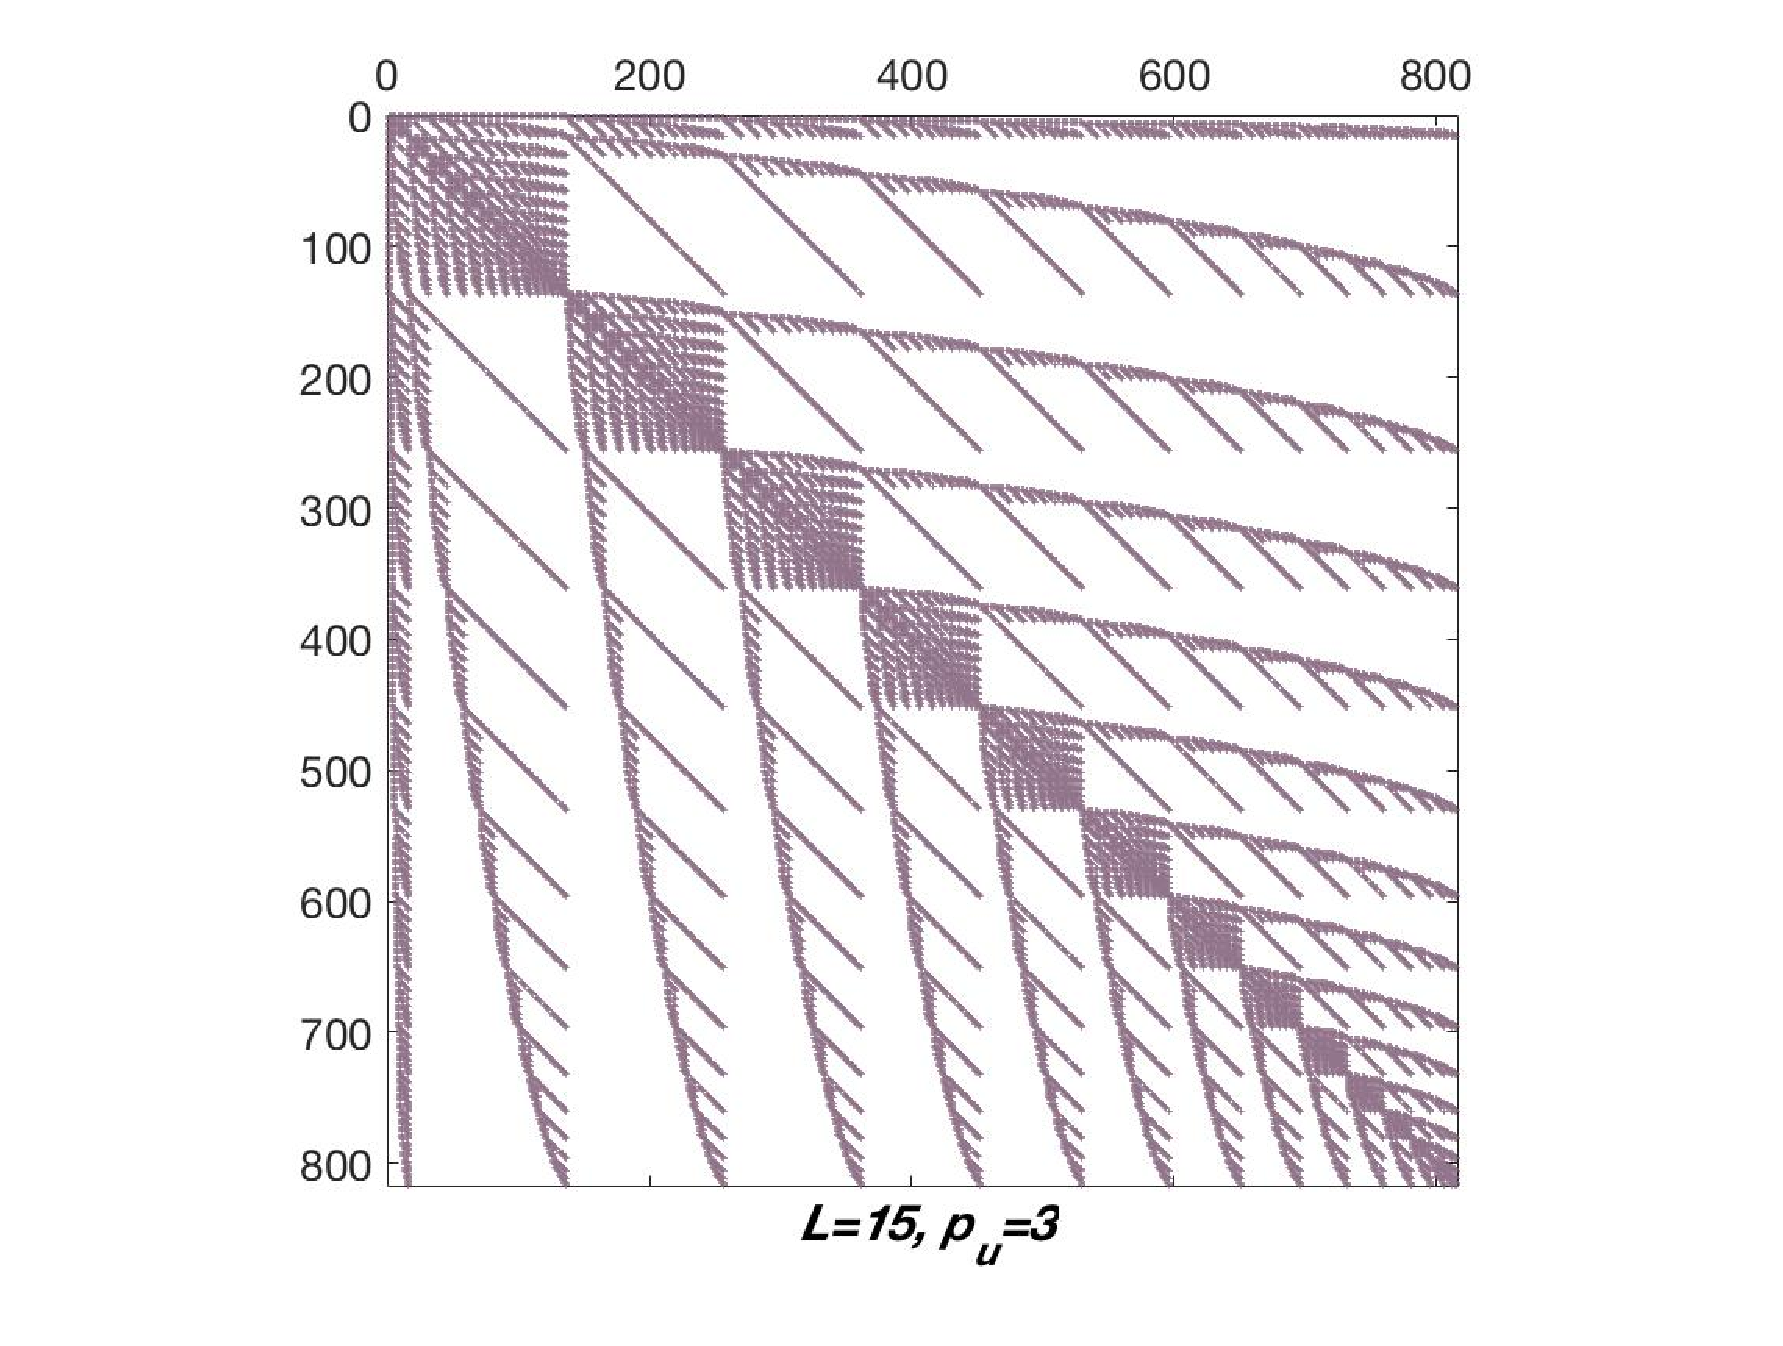
\includegraphics[width=0.32\textwidth,height=0.17\textheight]{plots/L15p3_n30.eps}
 \caption{SSFEM system matrices for the fixed $N=30$, $p_{\textsc{a}} = 2, p_{u} = 3$ with $L=5$, $L=10$ and $L=15$.}
 \label{fig:SFEM1}
\end{figure}
\begin{figure}[htbp]
\centering
 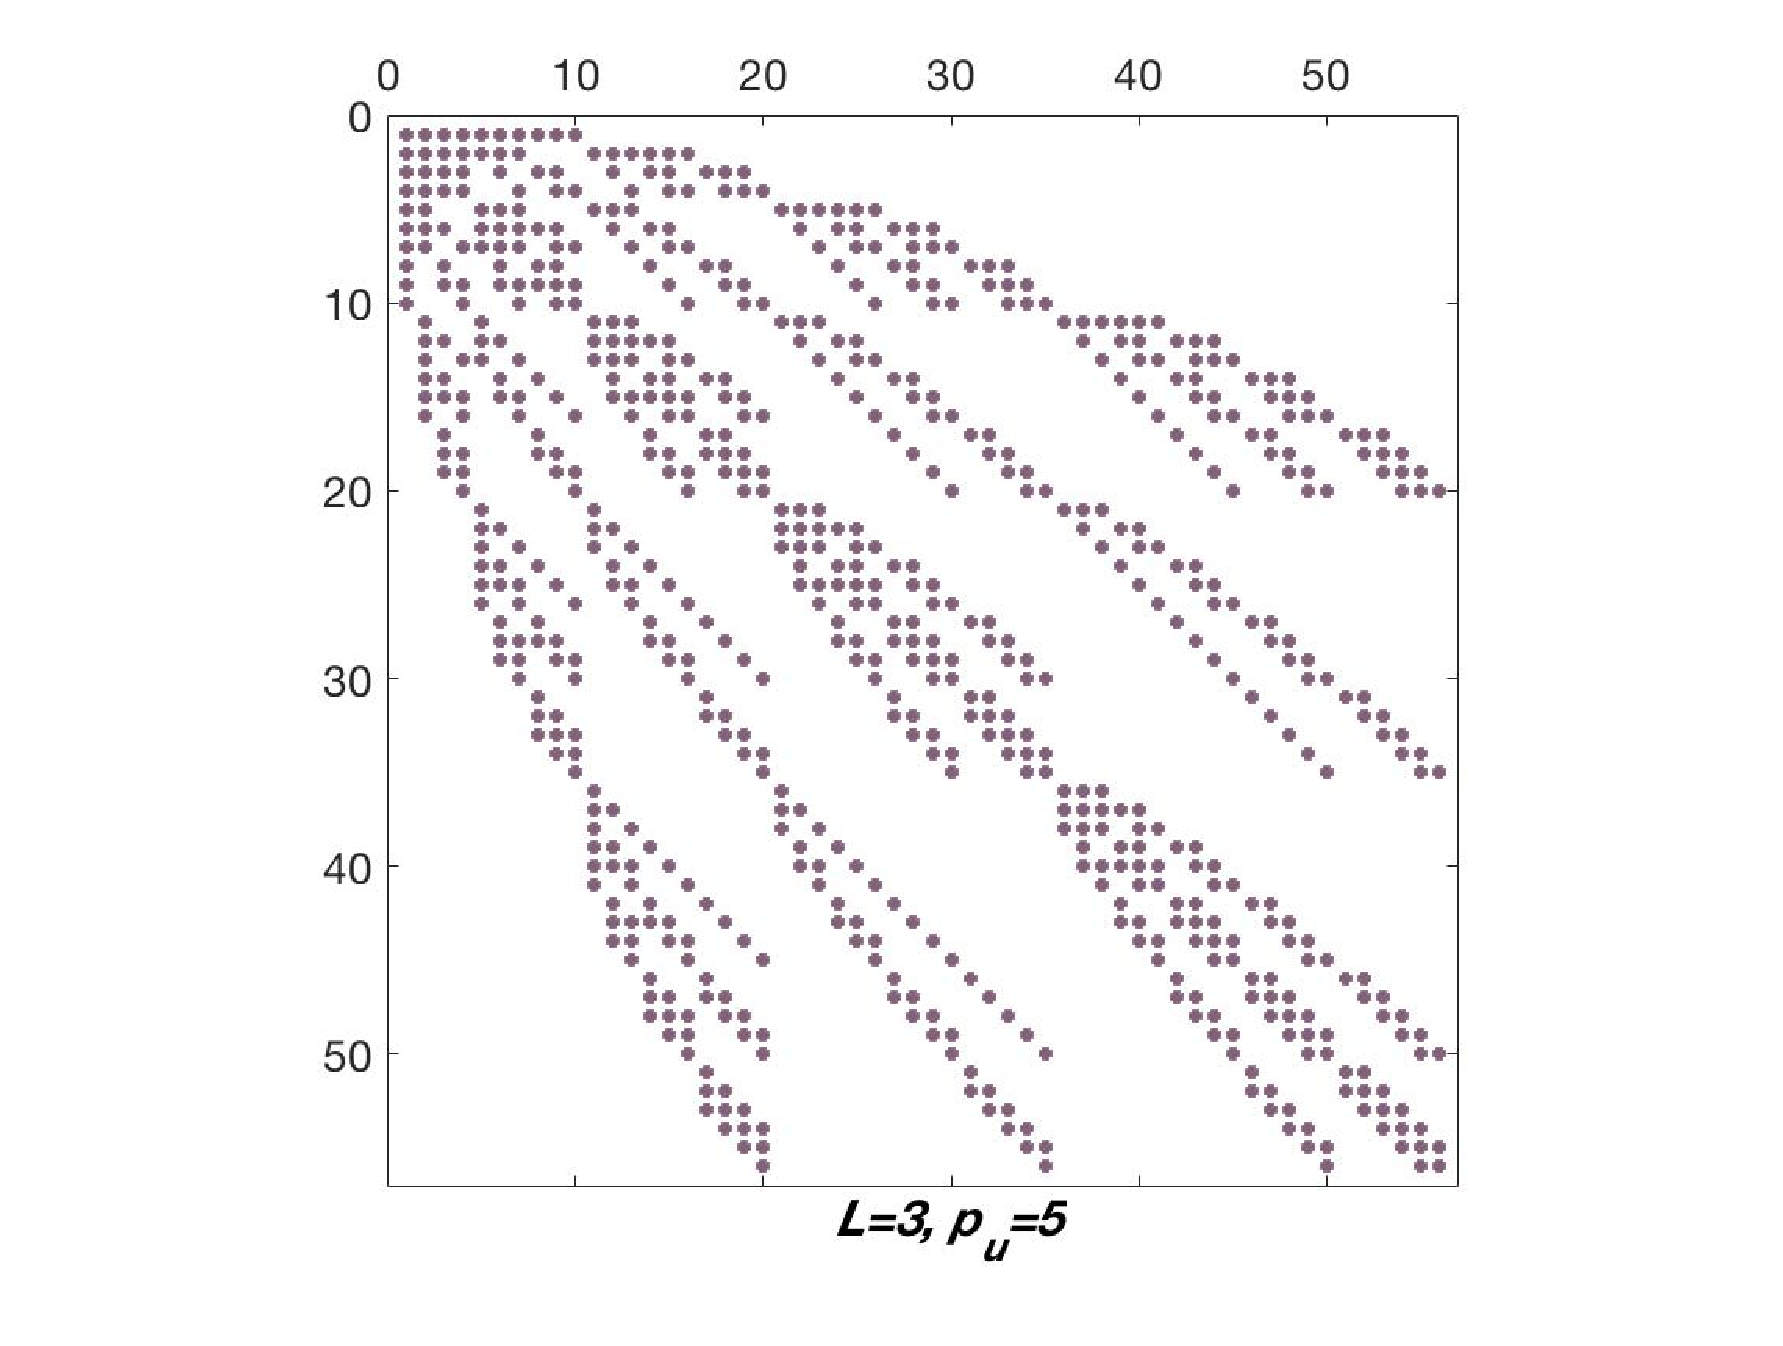
\includegraphics[width=0.32\textwidth,height=0.17\textheight]{plots/L3p5_n30.eps}
 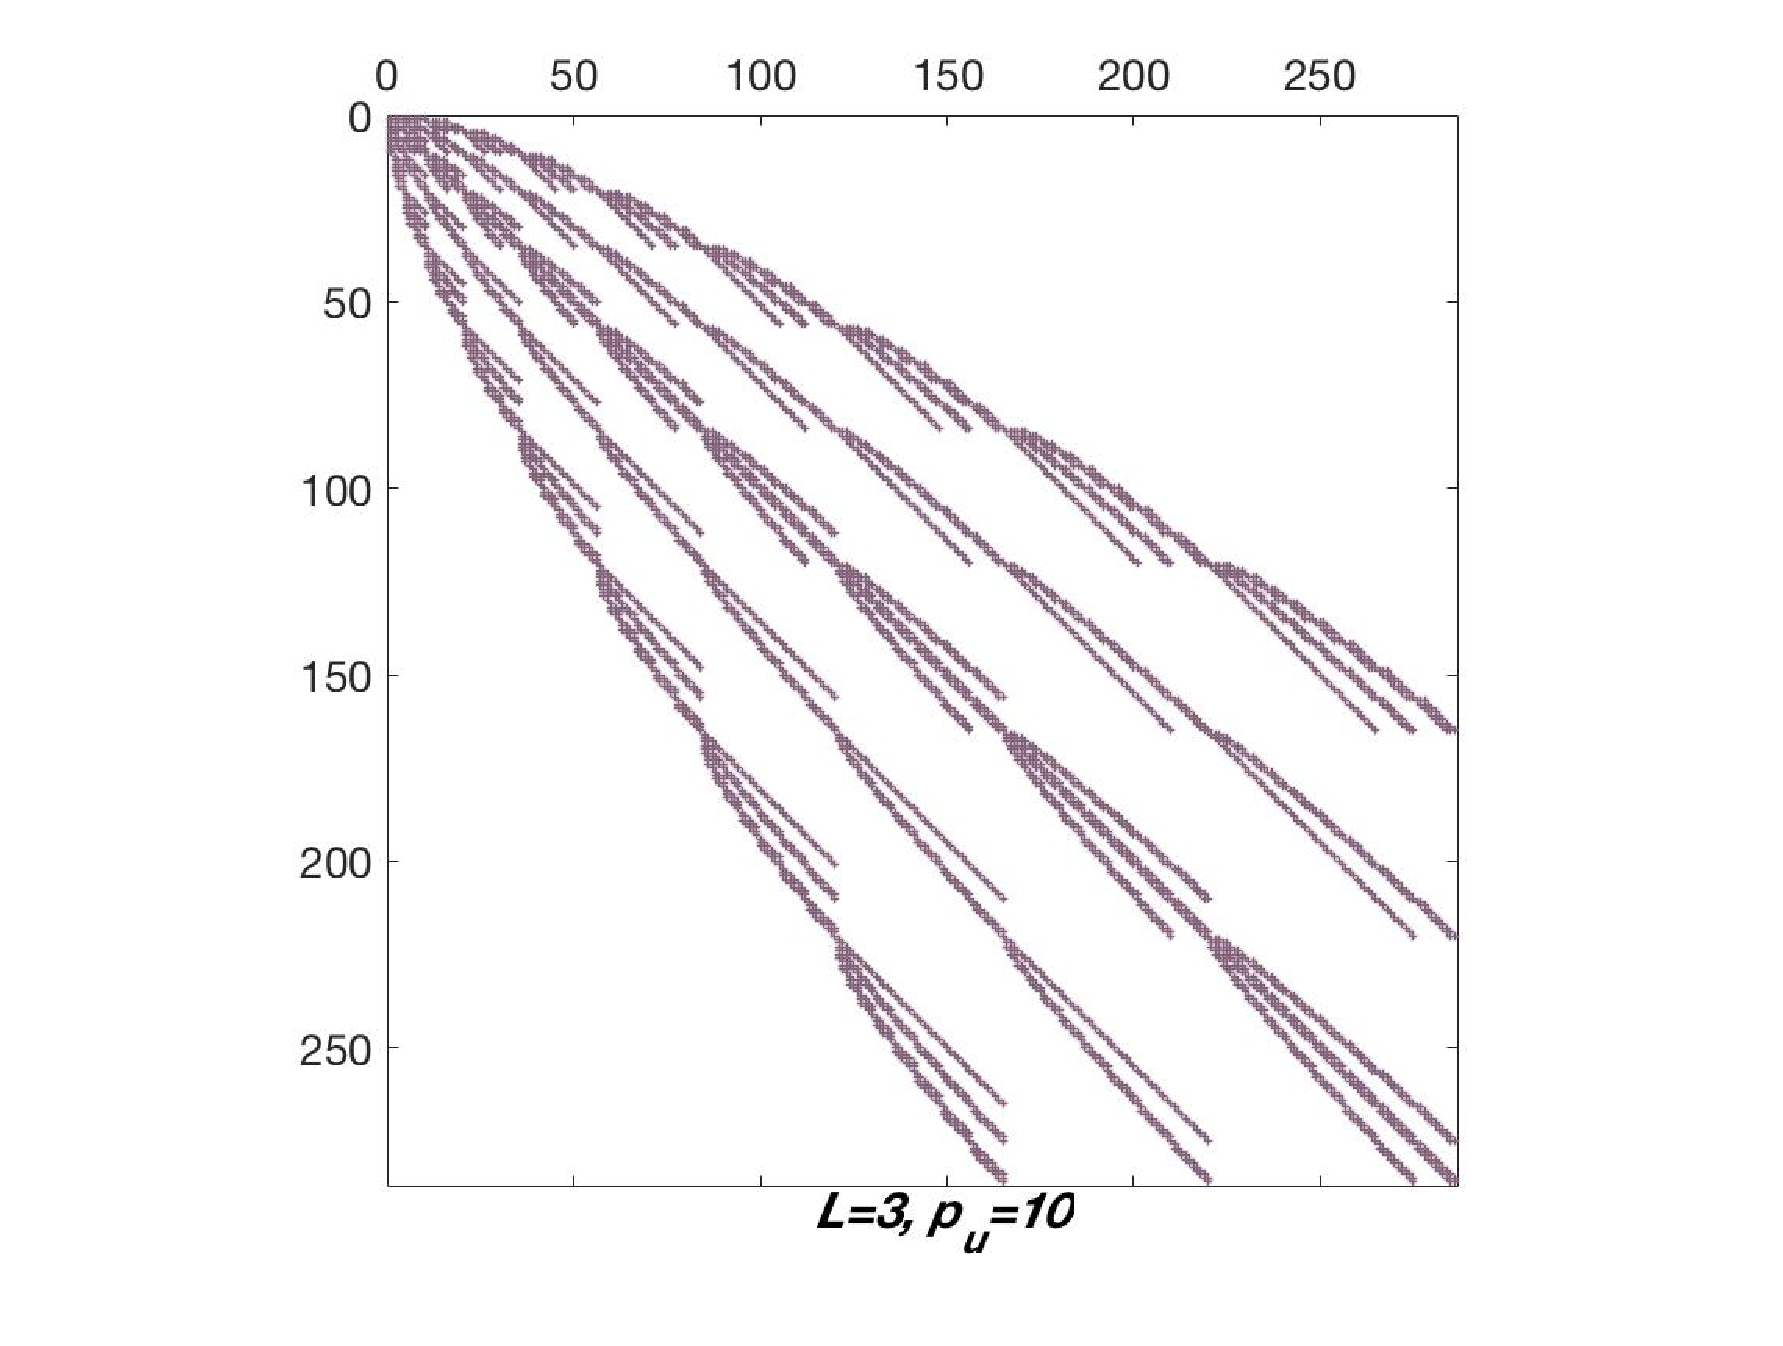
\includegraphics[width=0.32\textwidth,height=0.17\textheight]{plots/L3p10_n30.eps}
 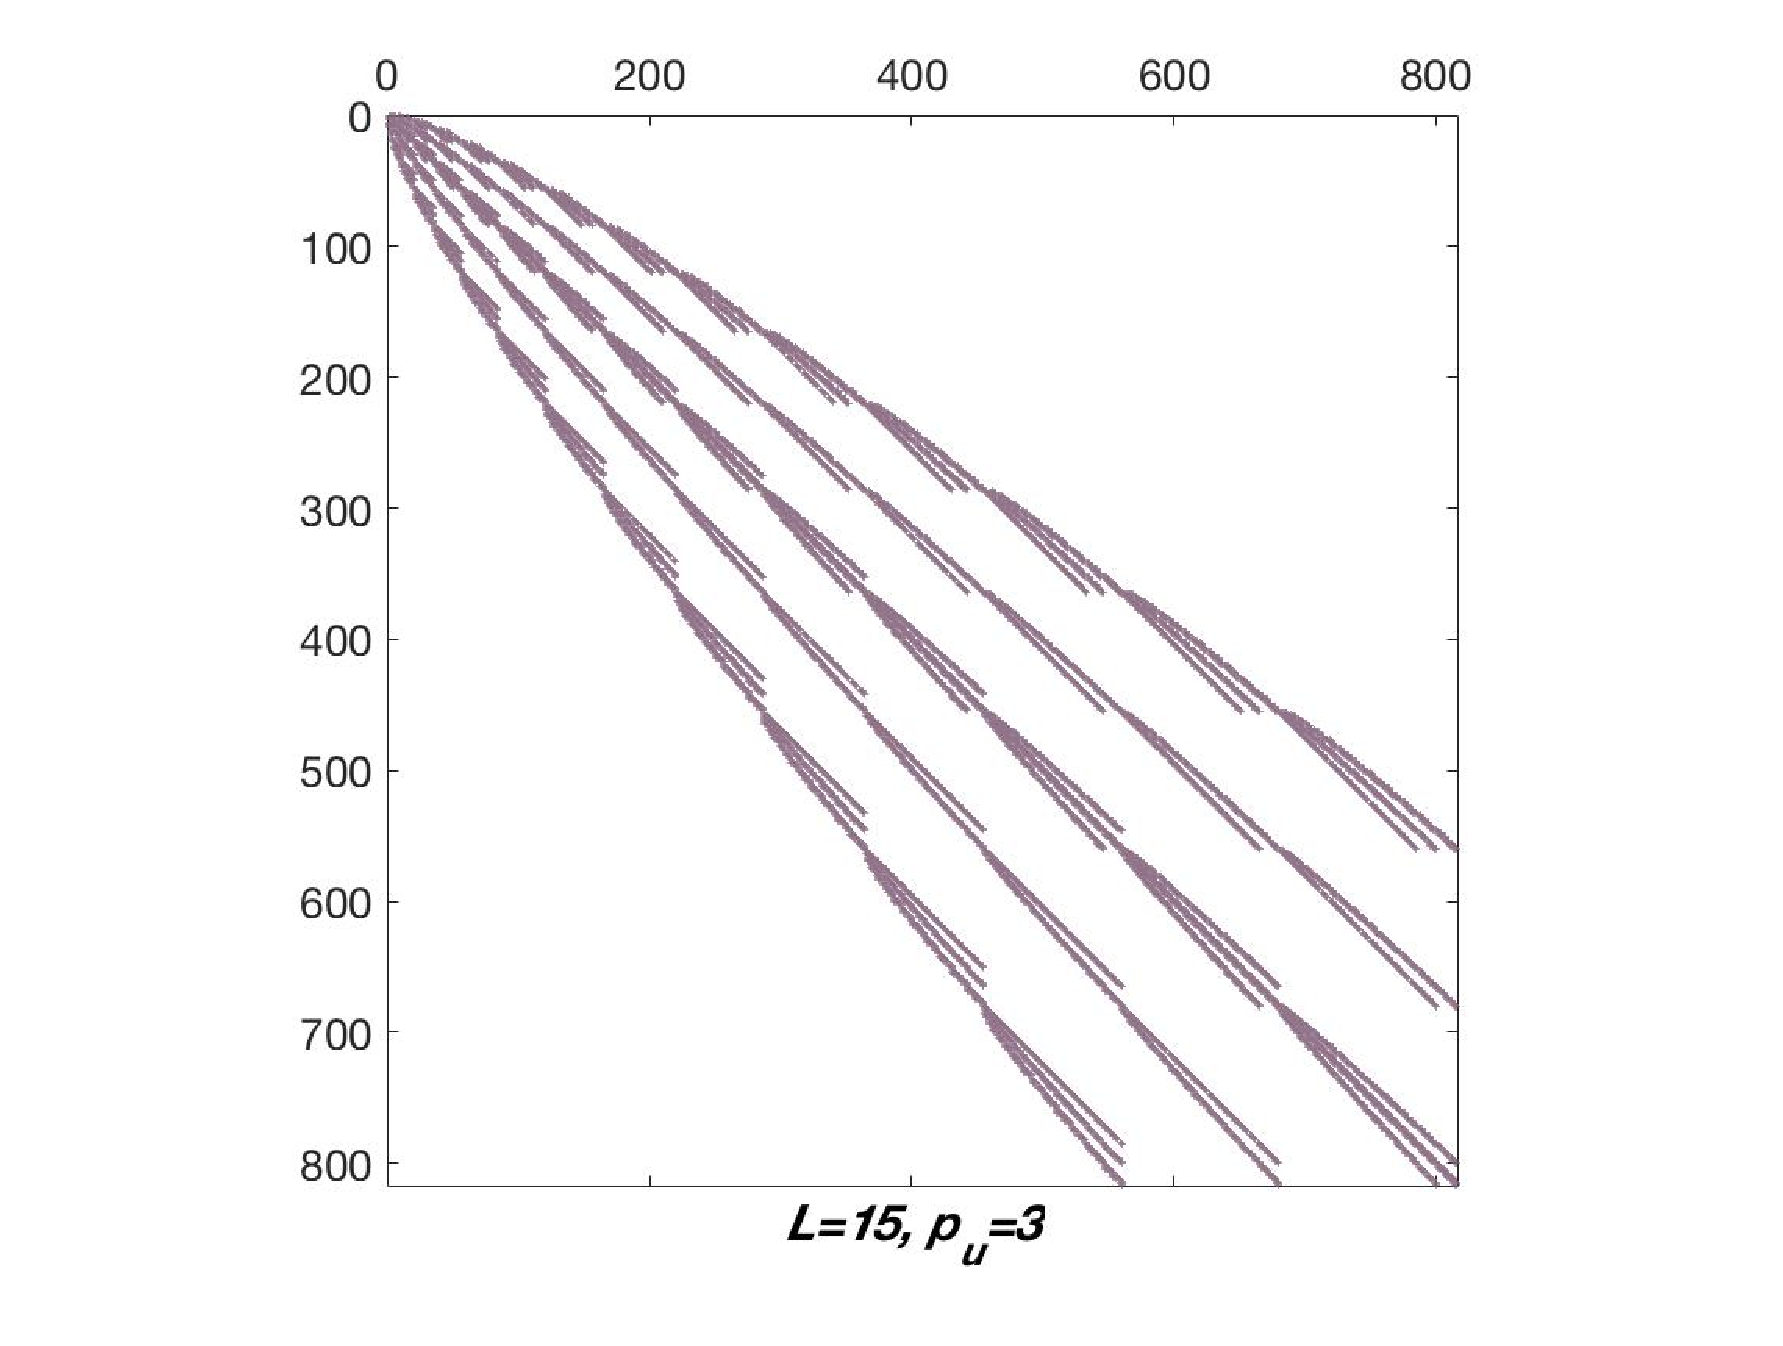
\includegraphics[width=0.32\textwidth,height=0.17\textheight]{plots/L3p15_n30.eps}
 \caption{SSFEM system matrices for the fixed $N=30$, $p_{\textsc{a}}=2, L=3$ with $p_{u}=5$, $p_{u}=10$ and $p_{u}=15$.}
 \label{fig:SFEM2}
\end{figure}
%---------------------------------------

The sparsity structure of each block ${\hat{{\mathrm{\bf{A}}}}_i}$ in the intrusive system matrix depends on finite element discretization. Therefore, its sparsity pattern is not influenced by stochastic expansion terms such as $L$ or $p_u$. However, the block-sparsity structure of the system matrix changes with (a) the number of random variables as shown in \Cref{fig:SFEM1} (for fixed order of expansion and varying number of random variables) and (b) the order of expansion as shown in \Cref{fig:SFEM2} (for fixed number of random variables and varying order of expansion). The orders and dimensions of the input and output stochastic processes influence the number of nonzero $\mathbfcal{C}_{ijk}$ terms, and thus the number of non-zero blocks in  $\mathcal{A}$. Consequently, the size of the intrusive system matrix and vector grows rapidly with the number of random variables and order of expansion.
%For example, as we increase the $L$ from 3 to 5 keeping $p_u=3$, the size of the matrix increases from ($600,600$) to ($1600,1600$) and number of nonzero elements increases from $30436$ to $139350$.
This is the primary challenge of the intrusive SSFEM with a large number of random variables and higher order expansions.
%The sparse data-structures can be employed to conveniently accommodate the size of intrusive system matrix and vector.
Another difficulty of this approach is the need for intrusive adjustments in the associated deterministic PDE solver. Thus the existing deterministic FEM package cannot be readily utilized; this makes the intrusive approach more complicated and demanding.
To overcome this challenge, in this paper the stochastic system assembly procedure is simplified by directly employing FEniCS deterministic assembly routines~\cite{logg2012FEniCS}.
%and routines to overcome the above challenges.
%For a fixed mesh resolution, as the stochastic dimension and/or polynomial order increases, the $P_{u}$ grows drastically. Hence, the size of the stochastic finite element matrix grows quickly and becomes the bottleneck of the method.

The implementational steps of intrusive SSFEM can be summarized as follows:
\begin{itemize}
\item Calculate and store the non-zero $\mathbfcal{C}_{ijk}$ terms, i.e., moments of multidimensional polynomials and their respective indices $i,j$ and $k$. This requires the computation of multidimensional inner products which can be obtained using one-dimensional moments and multi-indices~\cite{le2010spectral}. %(see~\Cref{apn:IN} for more details on multi-index).
The routines adopted from UQ Toolkit~\cite{debusschere2013uqtk} are employed to compute the $\mathbfcal{C}_{ijk}$ terms. %(see~\cite{desai2019scalable} for further details on the implementation along with code snippets).
%The detail implementation procedure with the code snippets is given in Appendix-B.
\item The intrusive system matrix $\mathcal{A}$ is assembled using the deterministic system matrices ${\hat{{\mathrm{\bf{A}}}}_i}$.
For each of the input PCE index $i$ in \Cref{eq:sFEMatrix}, the deterministic finite element assembly routines from an existing FEM package can be used to assemble ${\hat{{\mathrm{\bf{A}}}}_i}$. %(see~\cite{desai2019scalable} %\Cref{alg:smap_local} in~\Cref{apn:IN}
for details).
\item For the PCE indices $i, j$ and $k$ in \Cref{eq:sFEMatrix}, those matches with the pre-calculated non-zero $i, j$ and $k$ indices of $\mathbfcal{C}_{ijk}$, multiply the $i^{th}$ assembled deterministic matrix ${\hat{{\mathrm{\bf{A}}}}_i}$ with the respective $C_{ijk}$ and store it at the respective $[j,k]^{th}$ position of stochastic matrix $\mathcal{A}$.
\end{itemize}
Similar steps can be utilized to assemble the right hand side vector $\mathcal{F}$.
Further details on the FEniCS-based implementation of intrusive SSFEM along with the code snippets for each major step in the process are outlined in~\cite{desai2019scalable}. %\Cref{apn:IN}.
%The intrusive system matrix and vector assembly procedures are developed by utilizing the element-level deterministic assembly routines from the FEniCS~\cite{logg2012FEniCS}.
%The assembly procedure is designed to reduce the number of call to deterministic assembly routines and also to minimize the required memory by recursively using the available memory.
%Hence optimizing both memory and floating point operation count. Also the computational burden is reduced by invoking the calculations for a non-zero ${ijk}$ indices only.

%%## NI-SSFEM
%%%%%%%%%%%%%%%%%%%%%%%%%%%%%%%%%%%%%%%%%%%%%%
\subsection{Non-Intrusive SSFEM Approach} \label{sec:NI}
In this section, the PCE based non-intrusive spectral projection (NISP) approach is employed~~\cite{le2010spectral,reagana2003uncertainty,hosder2006non}.
%Another popular non-intrusive approach is stochastic collocation (SC)~\cite{} which is shown to perform.
In the NISP approach, the Galerkin projection is directly performed on the PCE of the solution process given in \Cref{eq:pceinout}. The orthogonality properties of PCE basis polynomials are utilized to compute the expansion coefficients of the solution process~\cite{ghanemSFEM1991,le2010spectral} as,
%Performing Galerkin projection onto the PCE expansion of solution process given in \Cref{eq:pce} and then exploiting orthogonality properties of the basis functions we get,
%\begin{equation}
% \left< {\mathrm{\bf{u}(\theta)}} {\Psi_k({\pmb{\xi}})}  \right>=  \sum^{P_{u}}_{j=0} {\mathrm{\hat{\bf{u}}}_j}  \left< {\Psi_j({\pmb{\xi}})} {\Psi_k({\pmb{\xi}})}  \right> \ , \ \ \ \ \   k = 0,..,P_{u}.
%\label{NIpce}
%\end{equation}
%Here $\left< {\Psi_j({\pmb{\xi}})} {\Psi_k({\pmb{\xi}})}  \right>$ exists only for $j=k$ otherwise it is zero.
%Next, each of the PCE coefficient of the solution process are evaluated independently using the sampled solutions from Eq.~\ref{nispSamp} as follows;
\begin{align}\label{eq:NISPpce}
{\mathrm{\hat{\bf{u}}}_k}   &= \frac{\left< {\mathrm{\bf{u}(\theta)}} {\Psi_k({\pmb{\xi}})}  \right>} {\left<{\Psi_k^2({\pmb{\xi}})}  \right>} \\ \nonumber &= \frac{1} {\left<{\Psi_k^2({\pmb{\xi}})}  \right>} \int_{\Omega} {\mathrm{\bf{u}(\theta)}} {\Psi_k({\pmb{\xi}})} {\mathrm{p}}({\pmb{\xi}}) {d{\pmb{\xi}}}.
\end{align}
The denominator in \Cref{eq:NISPpce} can be evaluated analytically beforehand
%(see~\cite{desai2019scalable} %\Cref{apn:validation} for examples).
Thus the major computational effort lies in the evaluation of the multidimensional integral in the numerator. In the past, random sampling, tensor product quadrature or sparse grid quadrature based approaches were employed to solve the above integral
%in the numerator of \Cref{eq:NISPpce}
~\cite{le2010spectral,reagana2003uncertainty,hosder2006non,ganapathysubramanian2007sparse,nobile2008sparse}.
%The efficient evaluation of the multidimensional integral in numerator of Eq.\ref{NISPpce} is key part in the implementation of of this NISP approach especially for the high dimensional stochastic cases.
The number of sampling points for random sampling and tensor product quadrature based approaches drastically increases with the increasing number of random variables and thereby renders these approaches inefficient~\cite{ganapathysubramanian2007sparse,nobile2008sparse,eldred2009comparison}. In such cases, the sparse grid quadrature (for example, ~\Cref{eq:sparseGridQuad}) can be used to reduce the number of the solution evaluation points while maintaining the same level of accuracy~\cite{le2010spectral,hosder2006non,ganapathysubramanian2007sparse,nobile2008sparse,eldred2009recent}.
\begin{align}\label{eq:sparseGridQuad}
  {\mathrm{\hat{\bf{u}}}_k} = \frac{1} {\left<{\Psi_k^2({\pmb{\xi}})}  \right>} \sum_{i=1}^{N_s} {{\omega}_p}_i {\mathrm{\bf{u}({\pmb{\xi}}}_i)} {\Psi_k({\pmb{\xi}}_i)},
\end{align}
where $N_s$ is the number of quadrature point with nodes ${\pmb{\xi}}_i$ and corresponding weights ${\omega_p}_i$ (which incorporates PDF ${\mathrm{p}}({\pmb{\xi}}_i)$).
In the current implementation, the Smolyak sparse grid quadrature scheme is employed to evaluate the integral in the numerator of \Cref{eq:NISPpce}~\cite{ganapathysubramanian2007sparse,nobile2008sparse,eldred2009recent,constantine2012sparse}.
For the sake of completeness we provide a minimal description of sparse grid techniques.  Numerous articles are available in the literature on the formulation of Smolyak sparse grid and its applications to SSFEM~\cite{ganapathysubramanian2007sparse,nobile2008sparse,eldred2009recent,eldred2009comparison,constantine2012sparse,smith2013uncertainty}.
%For further details we refer readers to the following articles~\cite{} and the references therein.

To illustrate the implementation of sparse grid quadrature based NISP approach, consider the finite element discretization of a stochastic PDE given in \Cref{eq:dFEM}. Using $\{ \pmb{\xi}_{1}, \pmb{\xi}_{2}, \dots, \pmb{\xi}_{n_{s}} \}$ the following deterministic system is solved at $N_s$ sample points (in this case, sparse quadrature points) using an existing deterministic solver:
\begin{equation}\label{eq:nispSamp}
{\mathrm{\bf{A}}}({\pmb{\xi}}_{i}(\theta))  {\mathrm{\bf{u}}}(\theta) = {\mathrm{\bf{f}}}, \ \ i = 1,\dots,N_s.
\end{equation}
The evaluated $\bf{u}(\theta)$ at each sample point ${\pmb{\xi}}_i$ is used in \Cref{eq:NISPpce} to calculate the PCE coefficients of the solution process.
%The various advanced sampling strategies were reported in past few years~[refer \cite{} articles and references therein].


The sparse grid quadrature rule to integrate a multidimensional function $\mathscr{F} = {\mathrm{\bf{u}(\theta)}} {\Psi_k({\pmb{\xi}})}$ in the numerator of \Cref{eq:NISPpce} %, i.e., $\int_{\Omega} {\mathrm{\bf{u}(\theta)}} {\Psi_k({\pmb{\xi}})} {\mathrm{p}}({\pmb{\xi}}) {d{\pmb{\xi}}}$
%${\mathscr{F}} = {\mathrm{\bf{u}(\theta)}} {\Psi_k({\pmb{\xi}})}$,
can be constructed using the univariate quadrature rule ${\mathscr{Q}}_{l}^{(1)} \mathscr{F}$ as follows ~\cite{eldred2009recent,smith2013uncertainty},
\begin{equation}\label{eq:sg1D}
{\mathscr{Q}}_{l}^{(1)} \ {\mathscr{F}} =  \sum_{q=1}^{N_{s}} {\mathscr{F}}(r_{l}^{q})  \ {w_p}^{q}_{l},
\end{equation}
where the subscript $l$ of ${\mathscr{Q}}$ is the level of quadrature and the superscript of ${\mathscr{Q}}$ denotes the dimension $d$ (in this case $d=1$). $N_{s}$ is the number of quadrature points in the sparse grid and %${\mathscr{F}} = {\mathrm{\bf{u}(\theta)}} {\Psi_k({\xi})}$.
$r_{l}^{q}$ and ${{w_p}^{q}_{l}}$
are the nodes and respective weights for the $l^{th}$ level sparse grid quadrature. The difference relation between two levels can be defined as~\cite{smith2013uncertainty}
\begin{equation}\label{eq:sparseDifference}
  \Delta_l^{(1)} {\mathscr{F}} = \Big( {\mathscr{Q}}_{l}^{(1)} - {\mathscr{Q}}_{l-1}^{(1)}  \Big)  {\mathscr{F}}
\end{equation}
where ${\mathscr{Q}}_{0}^{(1)} {\mathscr{F}} = 0$ and $\Delta_l^{(1)}{\mathscr{F}}$ is also a quadrature formula with the nodes same as ${\mathscr{Q}}_{l}^{(1)} {\mathscr{F}}$ and weights are difference between those at the levels $l$ and $l-1$. The set of nodal point for one-dimensional quadrature ${\mathscr{Q}}_{l}^{(1)} \mathscr{F}$ is denote by
\begin{equation}
  \Theta_{l}^{(1)} = \{ r_{l}^{1},\dots,r_{l}^{N_s} \}.
\end{equation}
For illustration of difference relation in~\Cref{eq:sparseDifference}, consider an example from~\cite{smith2013uncertainty}. The quadrature rule ${\mathscr{Q}}_{1}^{(1)}$ for $d=1$ and $l=1$ with the nodes $\Theta_{1}^{(1)}=\{ 0, 1 \}$ and weights = $\{ 0.5, 0.5 \}$. Similarly the quadrature rule ${\mathscr{Q}}_{2}^{(1)}$ for $l=2$ with the nodes $\Theta_{2}^{(1)}=\{ 0, 0.5, 1 \}$ and weights = $\{ 0.25, 0.5, 0.25 \}$. Then the nodes for the difference rule $\Delta_2^{(1)}$ are same as $\Theta_{2}^{(1)}= \{ 0, 0.5, 1 \}$, but the weights = $\{ -0.25, 0.5, -0.25 \}$ are obtained from the difference ${\mathscr{Q}}_{2}^{(1)} - {\mathscr{Q}}_{1}^{(1)}$.

The sparse grid formula for $d$-dimensional integral at level $l$ can be written using the difference relationship as~\cite{smith2013uncertainty}
\begin{equation}\label{eq:sgND}
{\mathscr{Q}}_{l}^{(d)} \ {\mathscr{F}} = \sum_{|l'| \leq l+d-1} \Big( {\Delta}_{l_1}^{(1)}  \otimes \dots \otimes {\Delta}_{l_d}^{(1)}  \Big) {\mathscr{F}}.
\end{equation}
where $l'=(l_1 \dots l_d)$ with $|l'| = \sum_{i=1}^d l_i$.
The nodal set $\Theta$ for the sparse grid can be obtained using one-dimensional sparse nodal set $\Theta_{l}^{(1)}$ as~\cite{smith2013uncertainty}
\begin{equation}\label{eq:sgNodes}
\Theta_{l}^{(d)} = \bigcup_{|l'| \leq l+d-1} \Big( \Theta_{l_1}^{(1)}  \times \dots \times \Theta_{l_d}^{(1)}  \Big),
\end{equation}
where $\bigcup$ denotes union of subsets.

For example, consider $\Theta_{1}^{(1)}$, $\Theta_{2}^{(1)}$  and $\Theta_{3}^{(1)}$ are the nodal sets at level $l=1,2$ and $3$ and dimension $d=1$. Then the sparse grid nodal set for $d=2$ and $l=3$ can be written as~\cite{smith2013uncertainty}
\begin{align}
  \Theta_{l=3}^{(d=2)} &= \bigcup_{|l'| \leq l+d-1} \Big( \Theta_{l_1}^{(1)}  \times \Theta_{l_2}^{(1)}  \Big) \\ \nonumber
  &= \Big( \Theta_{1}^{(1)}  \times \Theta_{1}^{(1)}  \Big) \ \ \ \ \ (l_1=1, l_2=1) \\ \nonumber &\cup \Big( \Theta_{1}^{(1)}  \times \Theta_{2}^{(1)}  \Big) \cup \Big( \Theta_{2}^{(1)}  \times \Theta_{1}^{(1)}  \Big) \\ \nonumber
  &\cup \Big( \Theta_{1}^{(1)}  \times \Theta_{3}^{(1)}  \Big)  \cup \Big( \Theta_{2}^{(1)}  \times \Theta_{2}^{(1)}  \Big)  \cup \Big( \Theta_{3}^{(1)}  \times \Theta_{1}^{(1)}  \Big).
\end{align}
Equivalent formulations of the Smolyak sparse grid using slightly different approach and also different notations can be found in the following articles~\cite{eldred2009recent,smith2013uncertainty,le2010spectral}.

% To simplify the notational complexity in \Cref{eq:sgND}, consider an example %E.g.1: if we expand the \Cref{eq:sgND} for $l=1$ and $d=2$ we get,
% % \begin{align}\label{eq:sgNDeg1}
% % {\mathscr{Q}}_{l=1}^{(d=2)} \ {\mathscr{F}} &= \Bigg( \sum_{i=1}^{l=1} \Big( {\mathscr{Q}}_{i}^{(1)} - {\mathscr{Q}}_{i-1}^{(1)}  \Big)  \otimes {\mathscr{Q}}_{1-i+1}^{(2-1)}  \Bigg) {\mathscr{F}}. \\
% % {\mathscr{Q}}_{1}^{(2)} \ {\mathscr{F}} &= \Bigg( \Big( {\mathscr{Q}}_{1}^{(1)} - {\mathscr{Q}}_{0}^{(1)}  \Big)  \otimes {\mathscr{Q}}_{1}^{(1)}  \Bigg) {\mathscr{F}}. \\
% % {\mathscr{Q}}_{1}^{(2)} \ {\mathscr{F}} &= \Bigg( {\mathscr{Q}}_{1}^{(1)}  \otimes {\mathscr{Q}}_{1}^{(1)}  \Bigg) {\mathscr{F}}. \label{eq:tensor}
% % \end{align}
% % \Cref{eq:tensor} is similar to the tensor product of two 1-D quadratures. For that reason, there are no benefits of using sparse-grid for low dimensions.
% with $l=2$ and $d=2$ to get~\cite{smith2013uncertainty},
% \begin{align}\label{eq:sgNDeg2}
% {\mathscr{Q}}_{l=2}^{(d=2)} \ {\mathscr{F}} &= \Bigg( \sum_{i=1}^{l=2} \Big( {\mathscr{Q}}_{i}^{(1)} - {\mathscr{Q}}_{i-1}^{(1)}  \Big)  \otimes {\mathscr{Q}}_{l-i+1}^{(2-1)}  \Bigg) {\mathscr{F}}, \\
% {\mathscr{Q}}_{2}^{(2)} \ {\mathscr{F}} &= \Bigg( \Bigg[ \Big( {\mathscr{Q}}_{1}^{(1)} - {\mathscr{Q}}_{0}^{(1)}  \Big)  \otimes {\mathscr{Q}}_{2}^{(2)}  \Bigg] + \Bigg[ \Big( {\mathscr{Q}}_{2}^{(1)} - {\mathscr{Q}}_{1}^{(1)}  \Big)  \otimes {\mathscr{Q}}_{1}^{(1)}  \Bigg]  \Bigg){\mathscr{F}}, \\ \label{eq:sgNDeg3}
% {\mathscr{Q}}_{2}^{(2)} \ {\mathscr{F}} &= \Bigg( \Bigg[ {\mathscr{Q}}_{1}^{(1)}  \otimes {\mathscr{Q}}_{2}^{(1)}  \Bigg]
% + \Bigg[ {\mathscr{Q}}_{2}^{(1)}  \otimes {\mathscr{Q}}_{1}^{(1)}  \Bigg] \Bigg) {\mathscr{F}}.
% \end{align}
% Similar procedure can be employed for higher-level and high-dimensional sparse grid construction. Further details with an example is given in~\Cref{apn:nisp}.
%The~\Cref{eq:sgNDeg3} can be used to construct multidimensional, higher-level sparse grid quadrature (see~\Cref{apn:nisp} for more details). %~\cite{smith2013uncertainty}.
%Equivalently, the Smolyak formula can also be written directly using $ \mathscr{U}^{(1)}_{l}$ as
% \begin{equation}\label{sg2}
%\mathscr{A}_{l}^{n} \ {\bf{u}_{f}}= \sum_{{(l+n)\leq |\mathrm{\bf{i}}|\leq}(l+n-1)}  (-1)^{(l+n)-{|\mathrm{\bf{i}}|}} \binom{n-1}{(l+n) - {|\mathrm{\bf{i}}|}} . (\mathscr{U}^{i_{1}} \otimes \dots \otimes\mathscr{U}^{i_{n}} )
%\end{equation}
%The level of quadrature $l$ is independent of dimension.
%The Smolyak formula is sparse tensor product formula (i.e. a fewer points are used in each dimension as compared to full tensor product grid).

For the implementation of the multidimensional sparse grid shown in \Cref{eq:sgND} the growth rule in one-dimensional quadrature given in \Cref{eq:sg1D} must be defined. The fully nested Clenshaw-Curtis abscissas~\cite{eldred2009recent,smith2013uncertainty} or the weakly-nested Gaussian abscissas~\cite{eldred2009recent,smith2013uncertainty} can be used.
%(see~\Cref{apn:nisp} for elementary example of these rules).
In the current implementation, we have used the Gaussian abscissas~\cite{eldred2009recent,smith2013uncertainty}.
For illustration, Smolyak sparse grid with the Gaussian abscissas for the two-dimensional case with $l=3$ and $l=6$ are showed in~\Cref{fig:sparseGrid} (see~\Cref{apn:nisp} for more details on sparse grid construction with Gaussian abscissas).
For a moderate dimension and the moderate level of quadrature, the sparse grid can drastically reduce the number of quadrature points compared to the tensor product grid~\cite{ganapathysubramanian2007sparse,nobile2008sparse,eldred2009comparison}. However, for high dimensional cases, the number of quadrature points substantially increases. For example,
%For low dimensions, i.e., $d=2$, the number of quadrature points increased from $13$ for $l=2$ to $89$ for $l=5$. For high dimensional cases, for instance
with $d=20$ the number of quadrature points increase from $841$ for $l=3$ to $1014809$ for $l=6$.
%, emphasizing the effect of dimensions.
For additional details on the types of growth rules and their performance comparisons for non-intrusive SSFEM, refer the following articles and reference therein~\cite{ganapathysubramanian2007sparse,nobile2008sparse,eldred2009recent,smith2013uncertainty}.

%-----------Abhi commented out------------
\begin{figure}[htbp]
\centering
 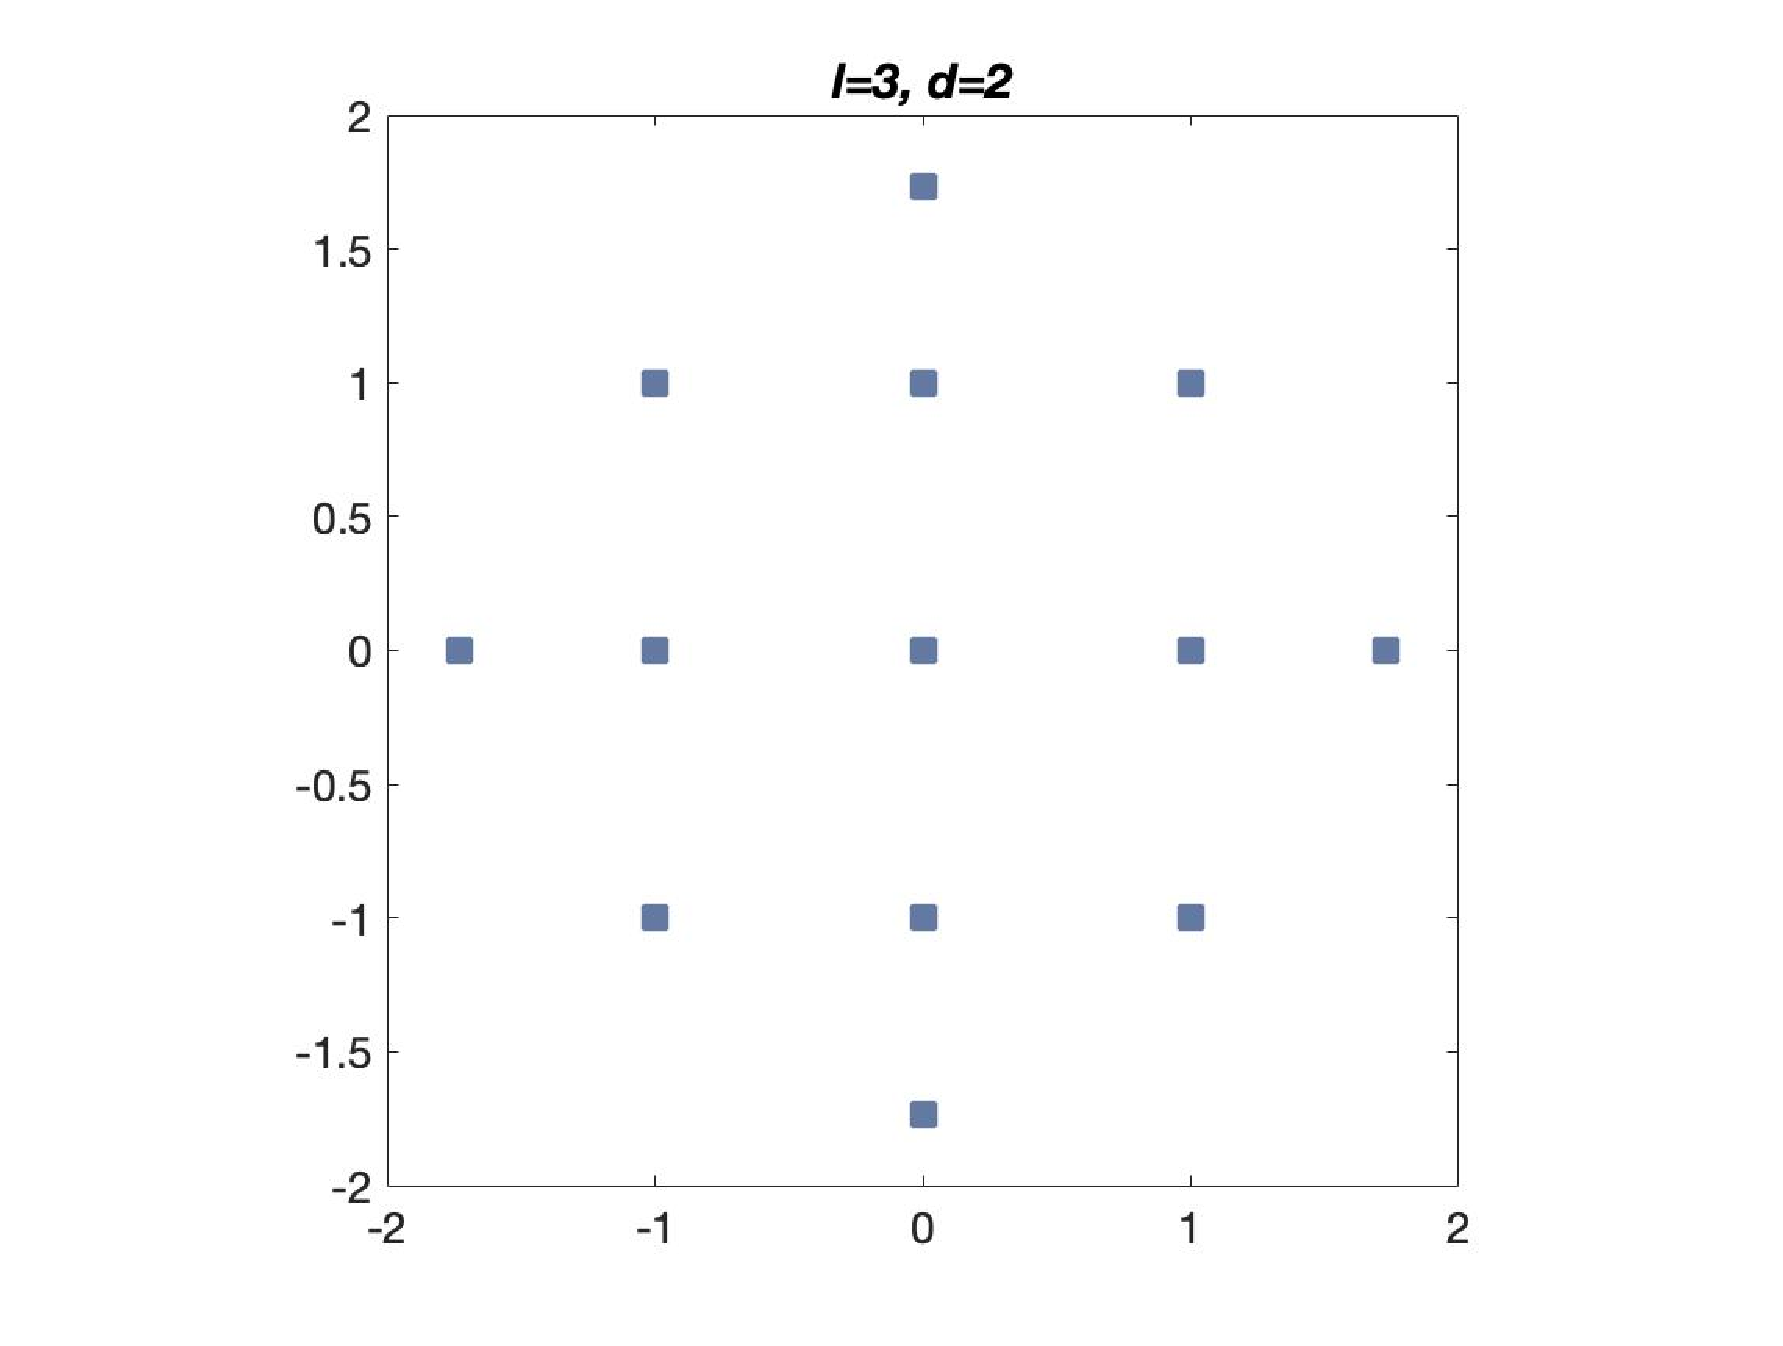
\includegraphics[width=0.48\textwidth,height=0.24\textheight]{plots/sparseGrid_D2L3.eps}
 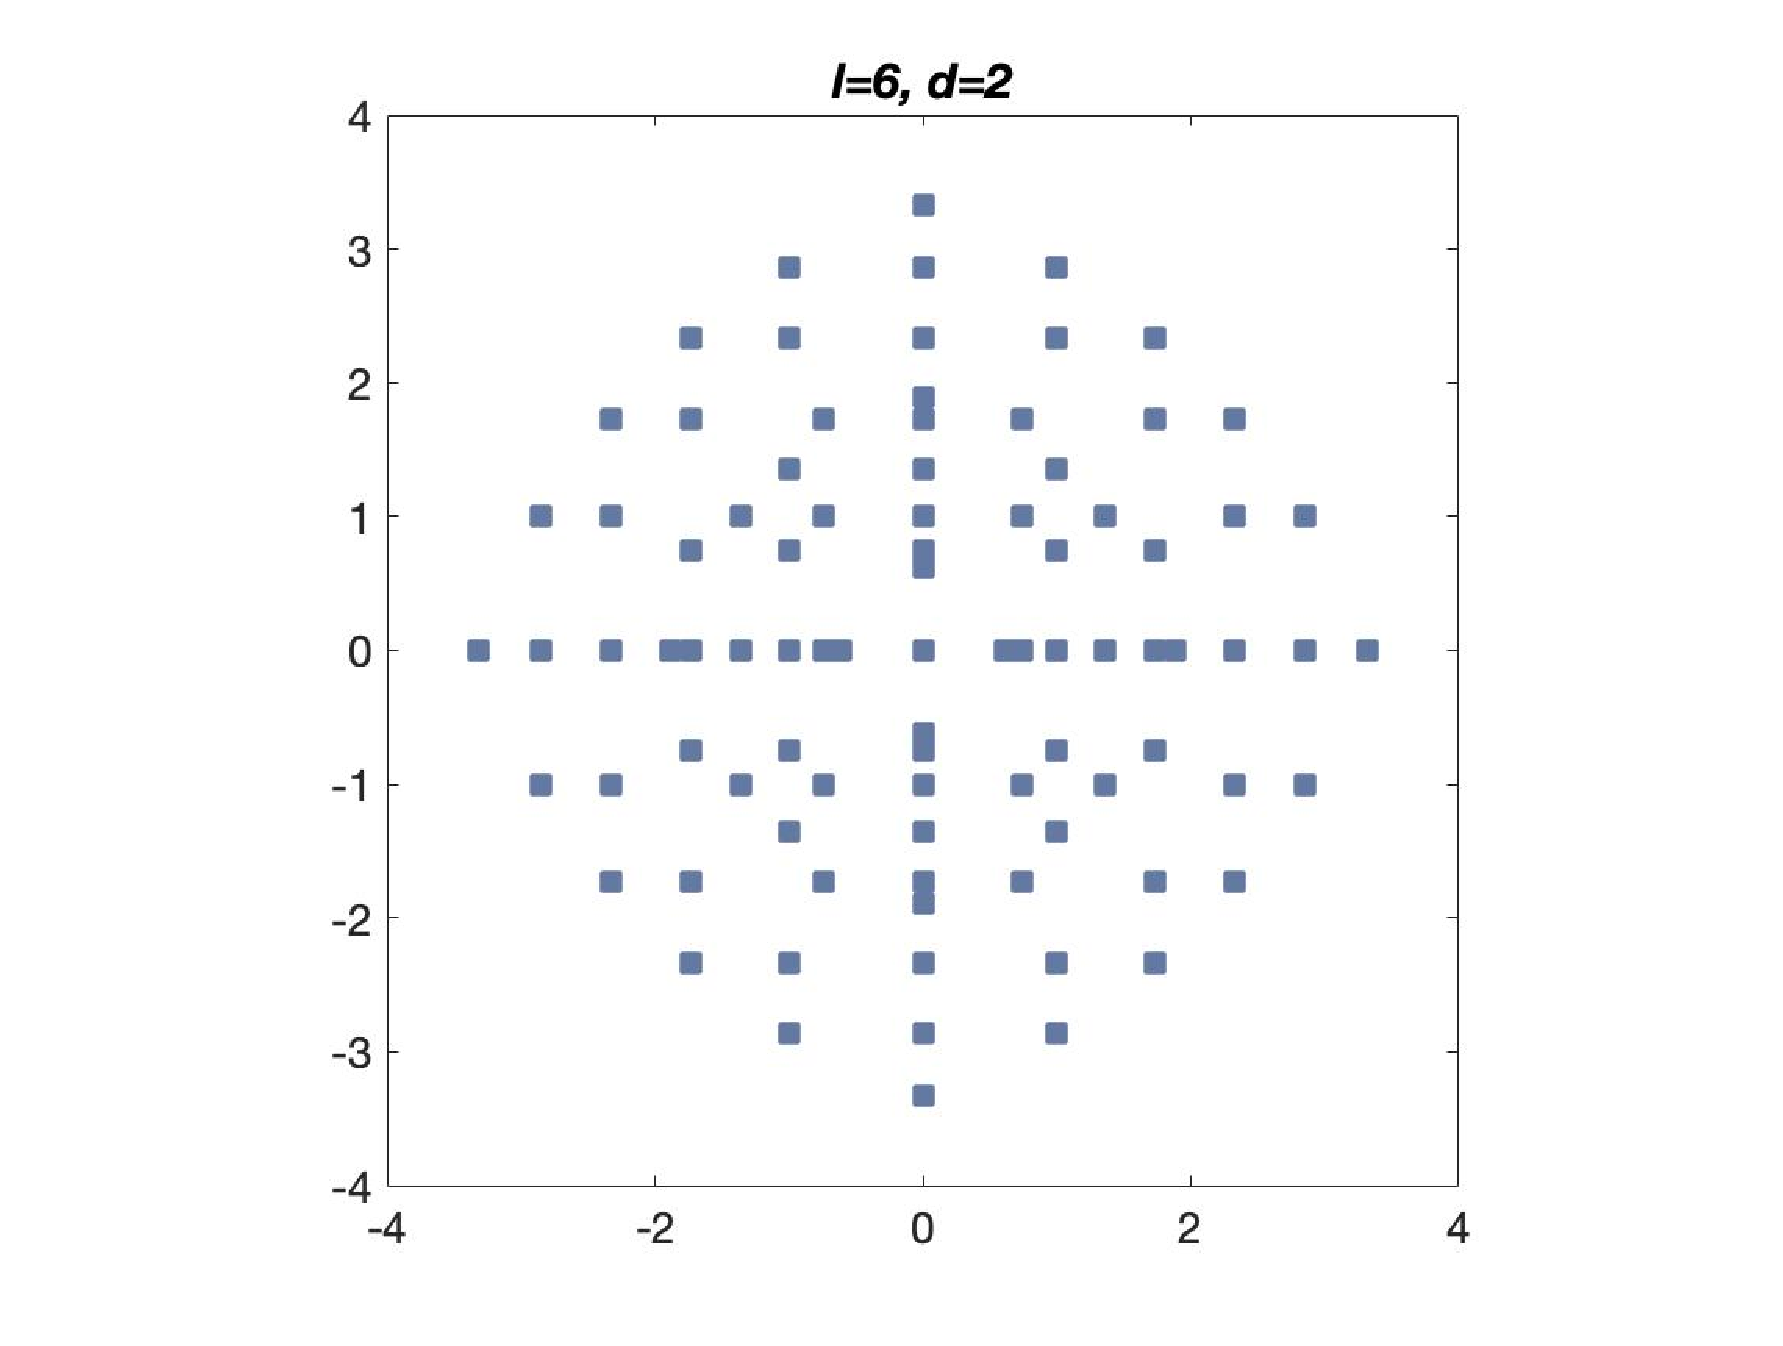
\includegraphics[width=0.48\textwidth,height=0.24\textheight]{plots/sparseGrid_D2L6.eps}
 \caption{Number of quadrature points for a fixed $d=2$ with $l=3$ and $l=6$.}
 \label{fig:sparseGrid}
\end{figure}
%----------------------------------------

The main advantage of the non-intrusive approach is that we do not have to modify the underlying deterministic PDE simulation code to use this method. Instead, the repetitive deterministic system solves are required at each sample point. This can be performed by directly employing any existing deterministic finite element solver as a black-box. Hence, the implementation of non-intrusive approaches demands a mush less coding effort than the intrusive approach. This feature makes the non-intrusive approaches more attractive option over the intrusive approach
~\cite{eldred2009comparison,elman2011assessment,tipireddy2010comparison,back2011stochastic,desai2010analysis}.
%However, %using the stochastic finite element matrix assembly procedure outlined in \Cref{alg:smap}, one can use an existing deterministic FEM assembly module to build the stochastic finite element matrix as discussed earlier ~\cite{ghanem1996numerical,pellissetti2000iterative}.
In this paper, the finite element solver from FEniCS FEM package~\cite{logg2012FEniCS,aloggs2013puffin} is employed to compute solution at the required samples. Further details on the implementation of NISP approach with the code snippets are outlined in~\Cref{apn:nisp}.
%%% Comments from eldred2009recent papers and adaptive sparse grid


\section{Comparison of Intrusive and Non-Intrusive SSFEM} \label{sec:inVni}
To the author's  best knowledge, there is no unanimous agreement in the UQ research community on which approach is superior: intrusive or non-intrusive method. Many articles suggest that the intrusive SSFEM method is more efficient concerning the accuracy and computational cost (albeit with substantial additional coding effort) as compared to the non-intrusive method for the following reasons~\cite{elman2011assessment,tipireddy2010comparison,stefanou2009stochastic,xiuNMSC2010,giraldi2014or}:
\begin{itemize}
\item To achieve the same level of accuracy, the computational cost of repeated system solution (e.g., at numerous quadrature points) of non-intrusive approach is considerably higher than that of the intrusive system arising from the stochastic Galerkin approach~\cite{elman2011assessment}.
\item The error due to the finite representation in intrusive approach is minimum leading to an optimal accuracy~\cite{ghanemSFEM1991}.
On the other hand,
%the error due to quadrature rules in non-intrusive approach can cause significant aliasing~\cite{ghanemSFEM1991,le2010spectral,elman2011assessment}.
%there is no explicit control of error in the non-intrusive approaches except at the sampling points where error is zero.
the accuracy of the non-intrusive approach highly depends on the choice of the sampling (quadrature, collocation) points~\cite{le2010spectral,xiuNMSC2010,back2011stochastic,eldred2009recent}.
For the large-scale applications where each deterministic simulation is computationally demanding the sampling-based non-intrusive approaches are computationally costly~\cite{elman2011assessment}. In such cases, the intrusive approach can be advantageous if an efficient intrusive system solver is employed~\cite{elman2011assessment}.
\end{itemize}

In this section, we implement both intrusive (SG) and non-intrusive (NISP) SSFEM approaches to compare their performances. The focus is given to compare the accuracies of these approaches for non-Gaussian random process modeling the stochastic system parameters with increasing number of random variables~\cite{ghanem1999nonlinear,ghanem1999stochastic}.
In the numerous assessments performed in the past, attention is given to the uniform or Gaussian random variables~\cite{elman2011assessment,back2011stochastic,desai2010analysis}. However, comparative studies for non-Gaussian random processes modeling the stochastic system parameters are not widely available in the literature.
%which are crucial for practical engineering applications were not performed.
Moreover, in this investigation, we conduct a detailed error analysis of the individual PCE coefficients along with the mean and variance of solution process to gain insights into the convergence behavior of both intrusive and non-intrusive approaches. This was lacking in the previous articles related to such assessments~\cite{elman2011assessment,tipireddy2010comparison,desai2010analysis}.
%in most of the past studies perform relate the final solution from intrusive and non-intrusive approaches~\cite{elman2011assessment,tipireddy2010comparison,desai2010analysis}. In this study, we perform error comparison in the individual PCE coefficients of solution process to get the further insights into the convergence behavior of both intrusive and non-intrusive approaches.
Note that, the adaptive PCE approaches reported in the literature~\cite{li1998adaptive,lucor2004adaptive,wan2005adaptive,nobile2008sparse} to lower the increased computational cost of the SSFEM approaches in high-dimensional stochastic spaces, are not considered in this paper. Note that, such adaptations can be exploited in both intrusive and non-intrusive setting~\cite{li1998adaptive,lucor2004adaptive,wan2005adaptive,nobile2008sparse}. Therefore, it may provide gains in both the approaches.
%which does not add any additional value to the comparative studies performed in this paper.
%, therefore, the similar effects are observed
But they are not pursued here although such studies will be worthy of future investigations.


Consider a two-dimensional steady-state flow through random media, modeled by a stochastic diffusion equation. This leads to a Poisson equation defined by a linear elliptic stochastic PDE as given in~\Cref{eq:sspe}. %on a spatial domain $\mathcal{D}$ with a Dirichlet boundary condition on $\partial \mathcal{D}$ as given in~\Cref{eq:sspe}.
% \begin{align}\label{eq:sspe_old}
% -\nabla \ \cdotp \big( \ c_d(\textbf{\textit{x}},\theta) \ \ \nabla u(\textbf{\textit{x}}, \theta) \ \big) &= {F}(\textbf{\textit{x}}),     \ \ \  \ \ \ \   \mathcal{D}\times \Omega, \\
% u(\textbf{\textit{x}}, \theta) &= 0,    \ \ \  \ \ \ \  \ \ \ \ \  \partial \mathcal{D}\times \Omega,
% \end{align}
% where $\nabla$ denotes the gradient which represents the differential operator with respect to the spatial variables $\textbf{\textit{x}}$, $F(\textbf{\textit{x}})$ is the deterministic forcing term, $u$ is the solution process,  $\theta$ is an element in the sample space $\Omega$ defined by the probability space ($\Omega, \mathcal{F}, \mathcal{P})$~\cite{billingsley2008probability}.
% where $\mathcal{F}$ is the $\sigma$-algebra and $\mathcal{P}$ is the probability measure .
The diffusion coefficient $c_d(\textbf{\textit{x}},\theta)$ is modeled as a lognormal stochastic process obtained by an exponential of a Gaussian process having the mean $g(\textbf{\textit{x}})=0$, standard deviation $\sigma=0.4$ and the exponential covariance function $C_{\alpha\alpha}$ (given in \Cref{eq:exp2d}) with correlation lengths $b_{1} = b_{2} = 1.0$. The lognormal process representation ensures that the diffusion coefficient $c_d$ remains positive over the entire domain.
The physical domain with unit-square geometry is discretized using an unstructured finite element mesh with $N=133$ nodes and $264$ linear triangular elements.
%A typical mesh with $102010$ nodes and $202910$ triangular elements partitioned into $48$ subdomains is shown in \Cref{fig:DDmesh}.

The PCE representations from \Cref{eq:pce} are used for the uncertain system parameters and the solution process. The procedure outlined in the \Cref{sec:IN} is followed to formulate the intrusive SSFEM system given in the form of \Cref{eq:sFEM}. The PCE coefficients of the solution process are obtained by directly solving the intrusive system given in \Cref{eq:sFEM}. Similarly, the non-intrusive procedure discussed in \Cref{sec:NI} is employed to obtain the solution coefficients from \Cref{eq:NISPpce}. The required deterministic samples for the sparse grid quadratures are computed by directly solving \Cref{eq:nispSamp}. Note that the results presented in this section are obtained by employing a direct serial solver for both intrusive and non-intrusive SSFEM.
%A stochastic finite element assembly matrix $\mathcal{[A]}$ (from \Cref{eq:sFEM}) for intrusive approach for $p_{A} = 2$ and $p_{u} = 3$ with $L=3$ is show in \Cref{}. Similarly, the finite element assembly matrix for one sample of non-intrusive approach for $p_{A} = 2$ and $p_{u} = 3$ with $L=3$ is show in \Cref{}.
% In both the approaches a direct solver is employed to solve the system of equations
%The primary focus is given to compare the performance of the both these approaches with increasing stochastic dimensions.

%--------------Abhi commented out------------------
\begin{figure}[htbp]
\centering
 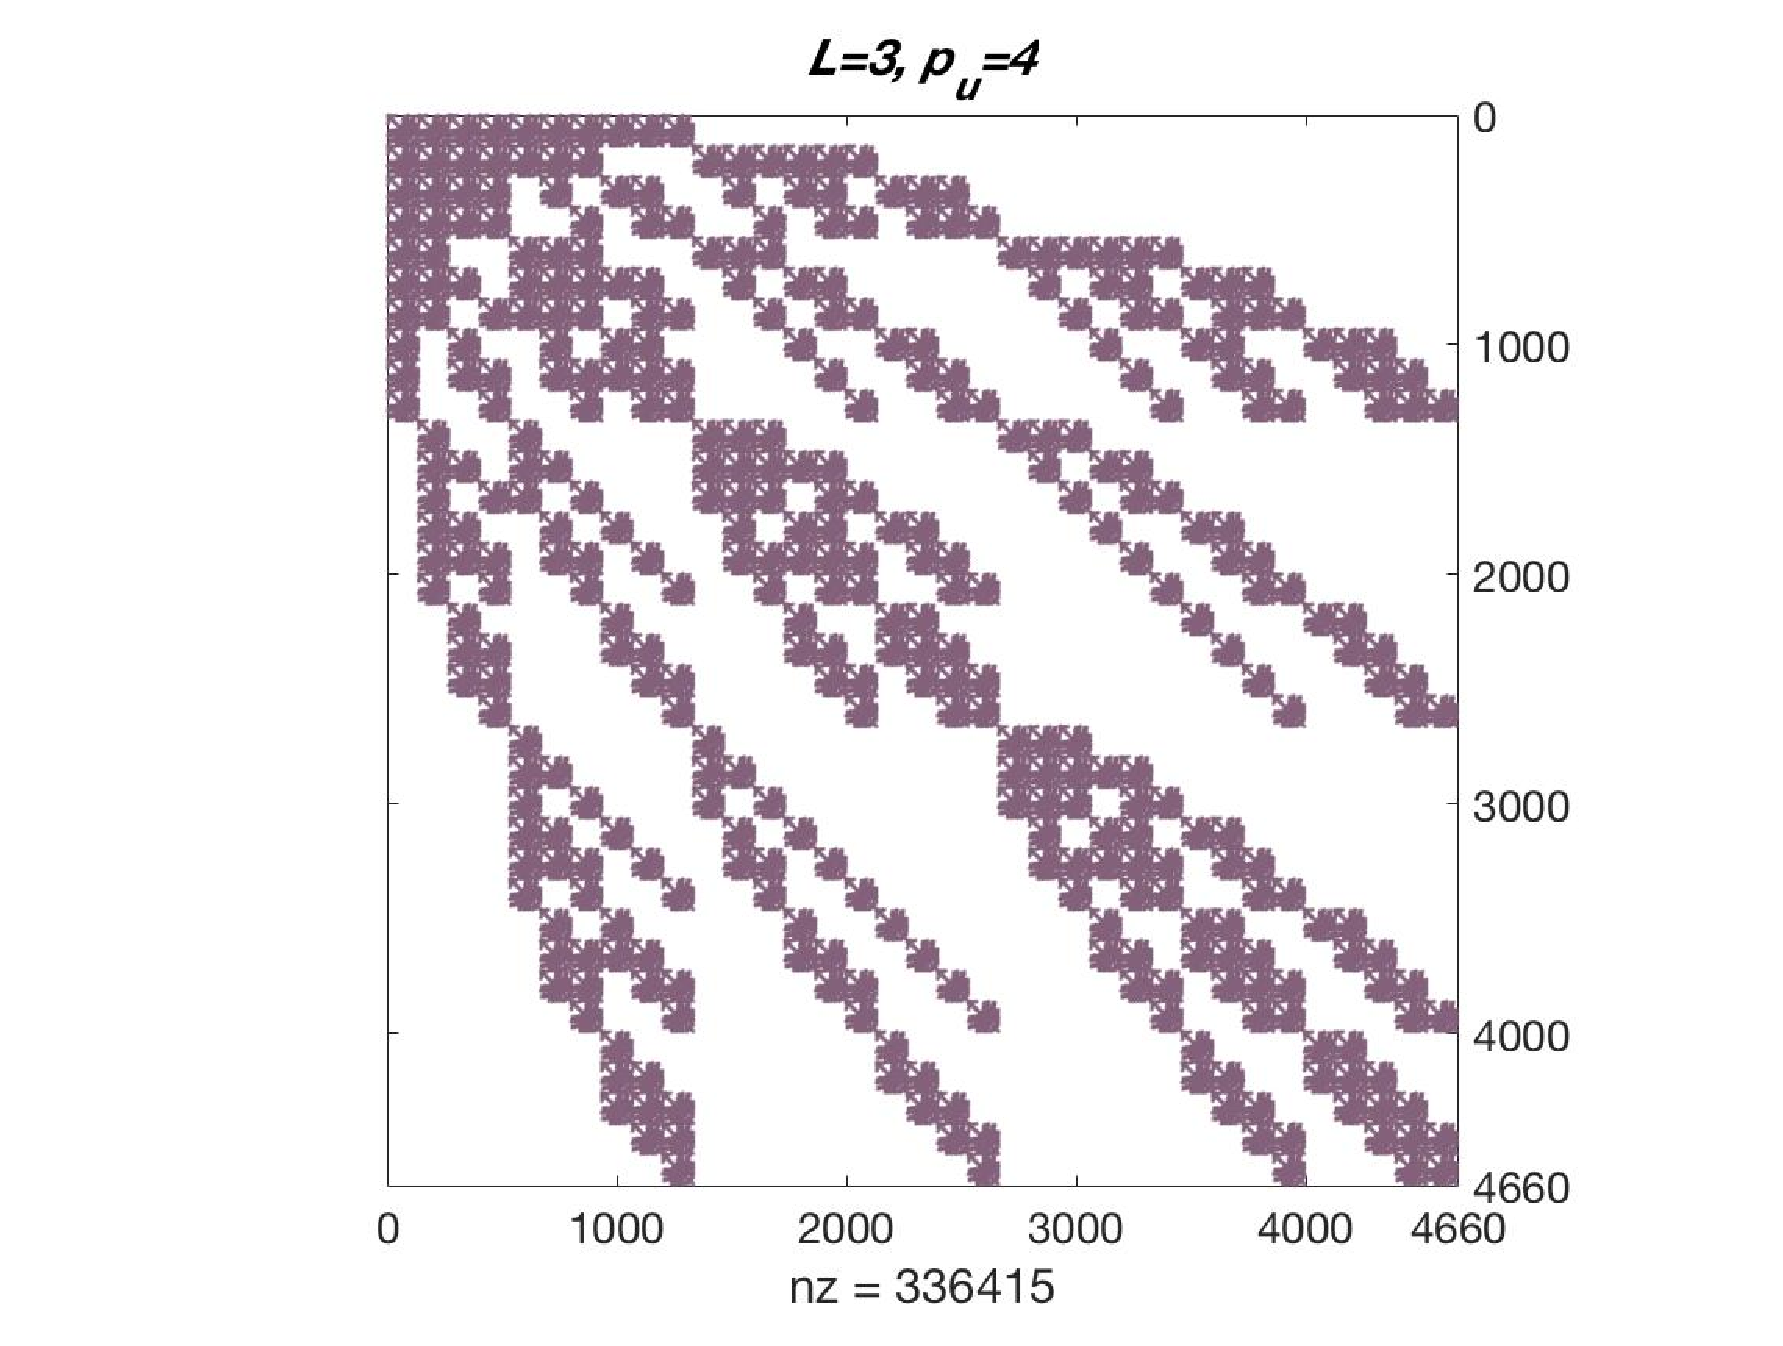
\includegraphics[width=0.49\textwidth,height=0.26\textheight]{plots/L3p4.eps}
 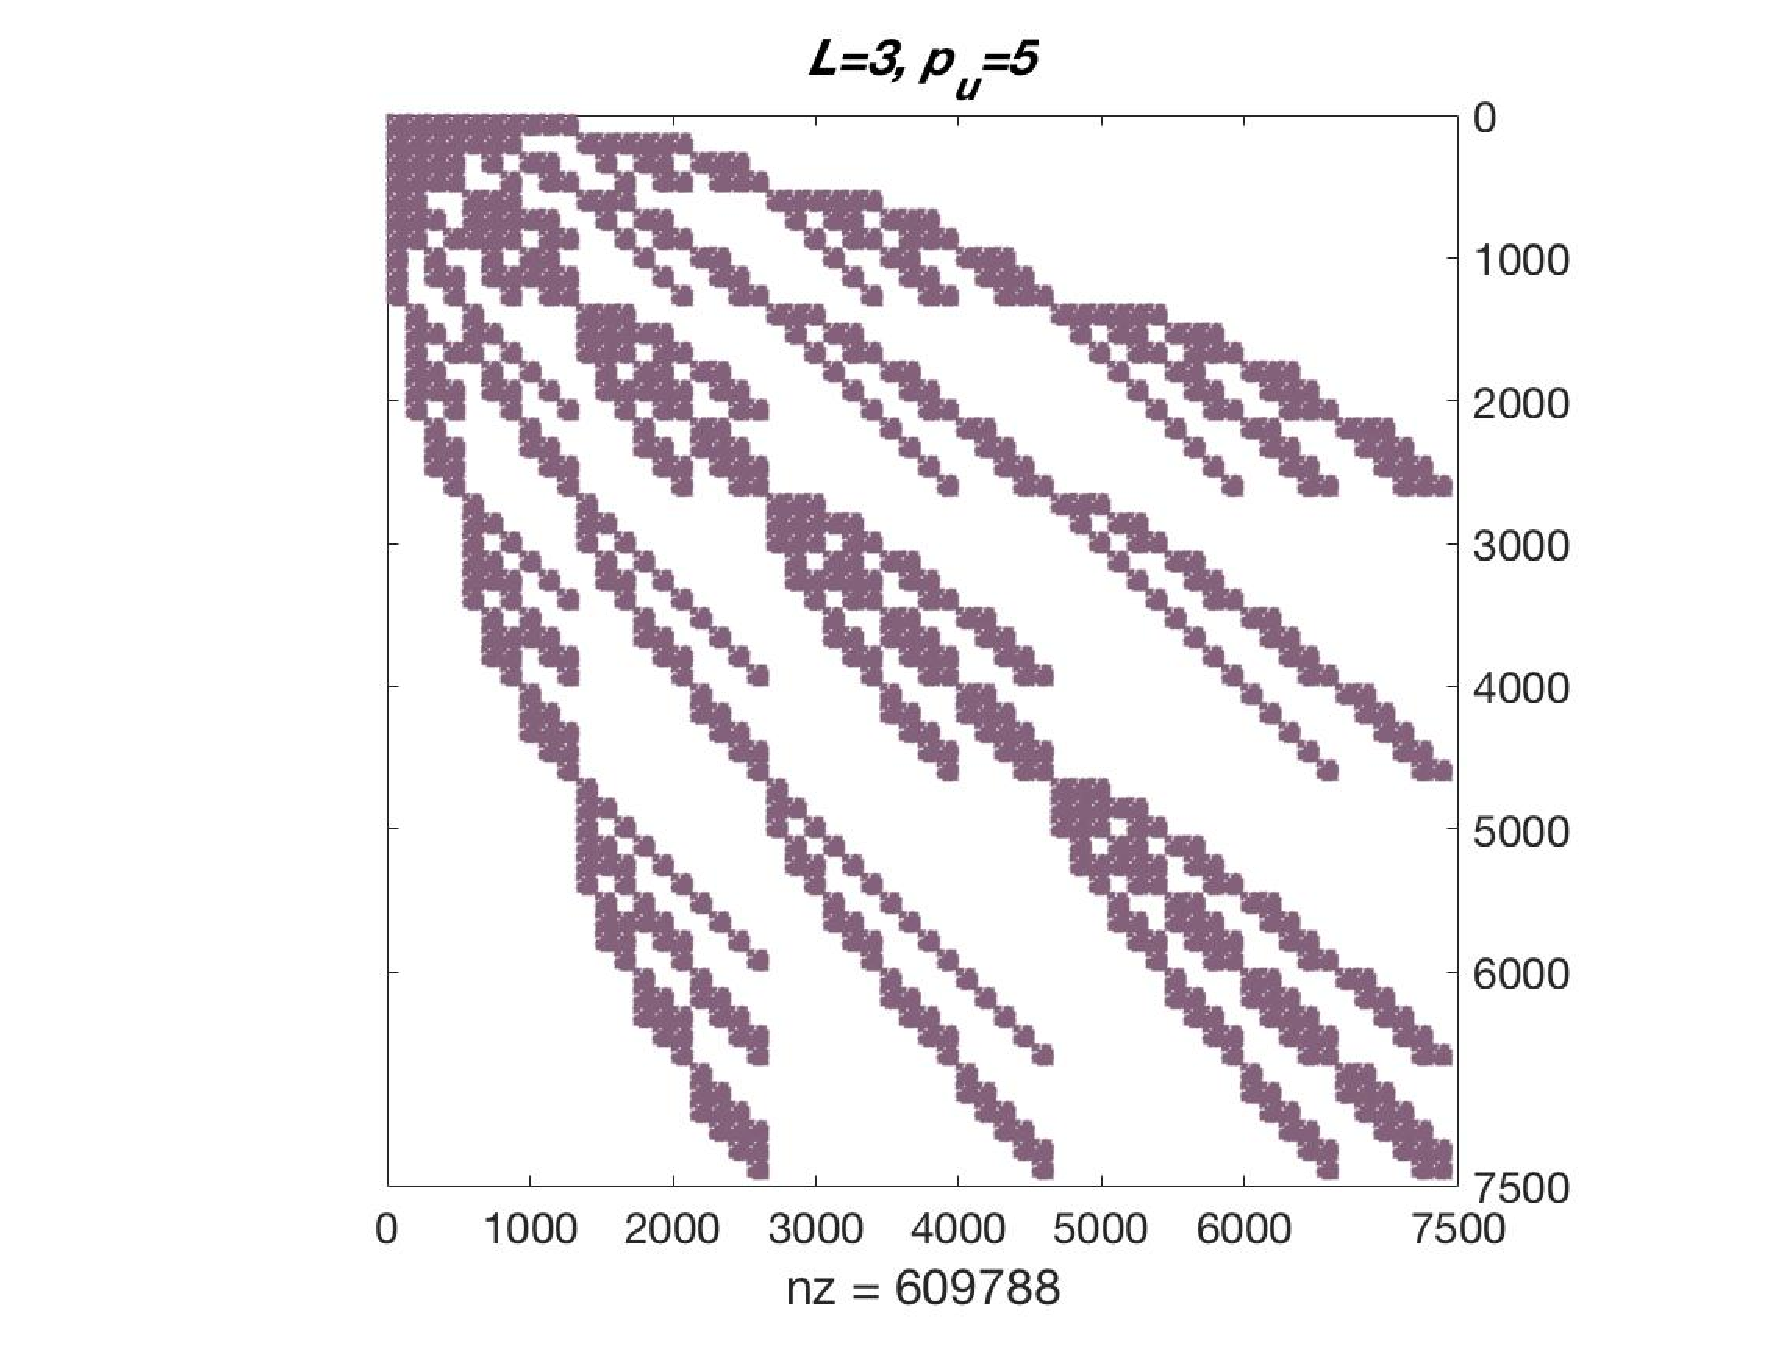
\includegraphics[width=0.49\textwidth,height=0.26\textheight]{plots/L3p5.eps}
 \caption{Block-sparse structures of the intrusive system matrices for a fixed mesh resolution with $L=3$ and $p_{u}=4,5$}
 \label{fig:sFEMord}
\end{figure}
\begin{figure}[htbp]
\centering
 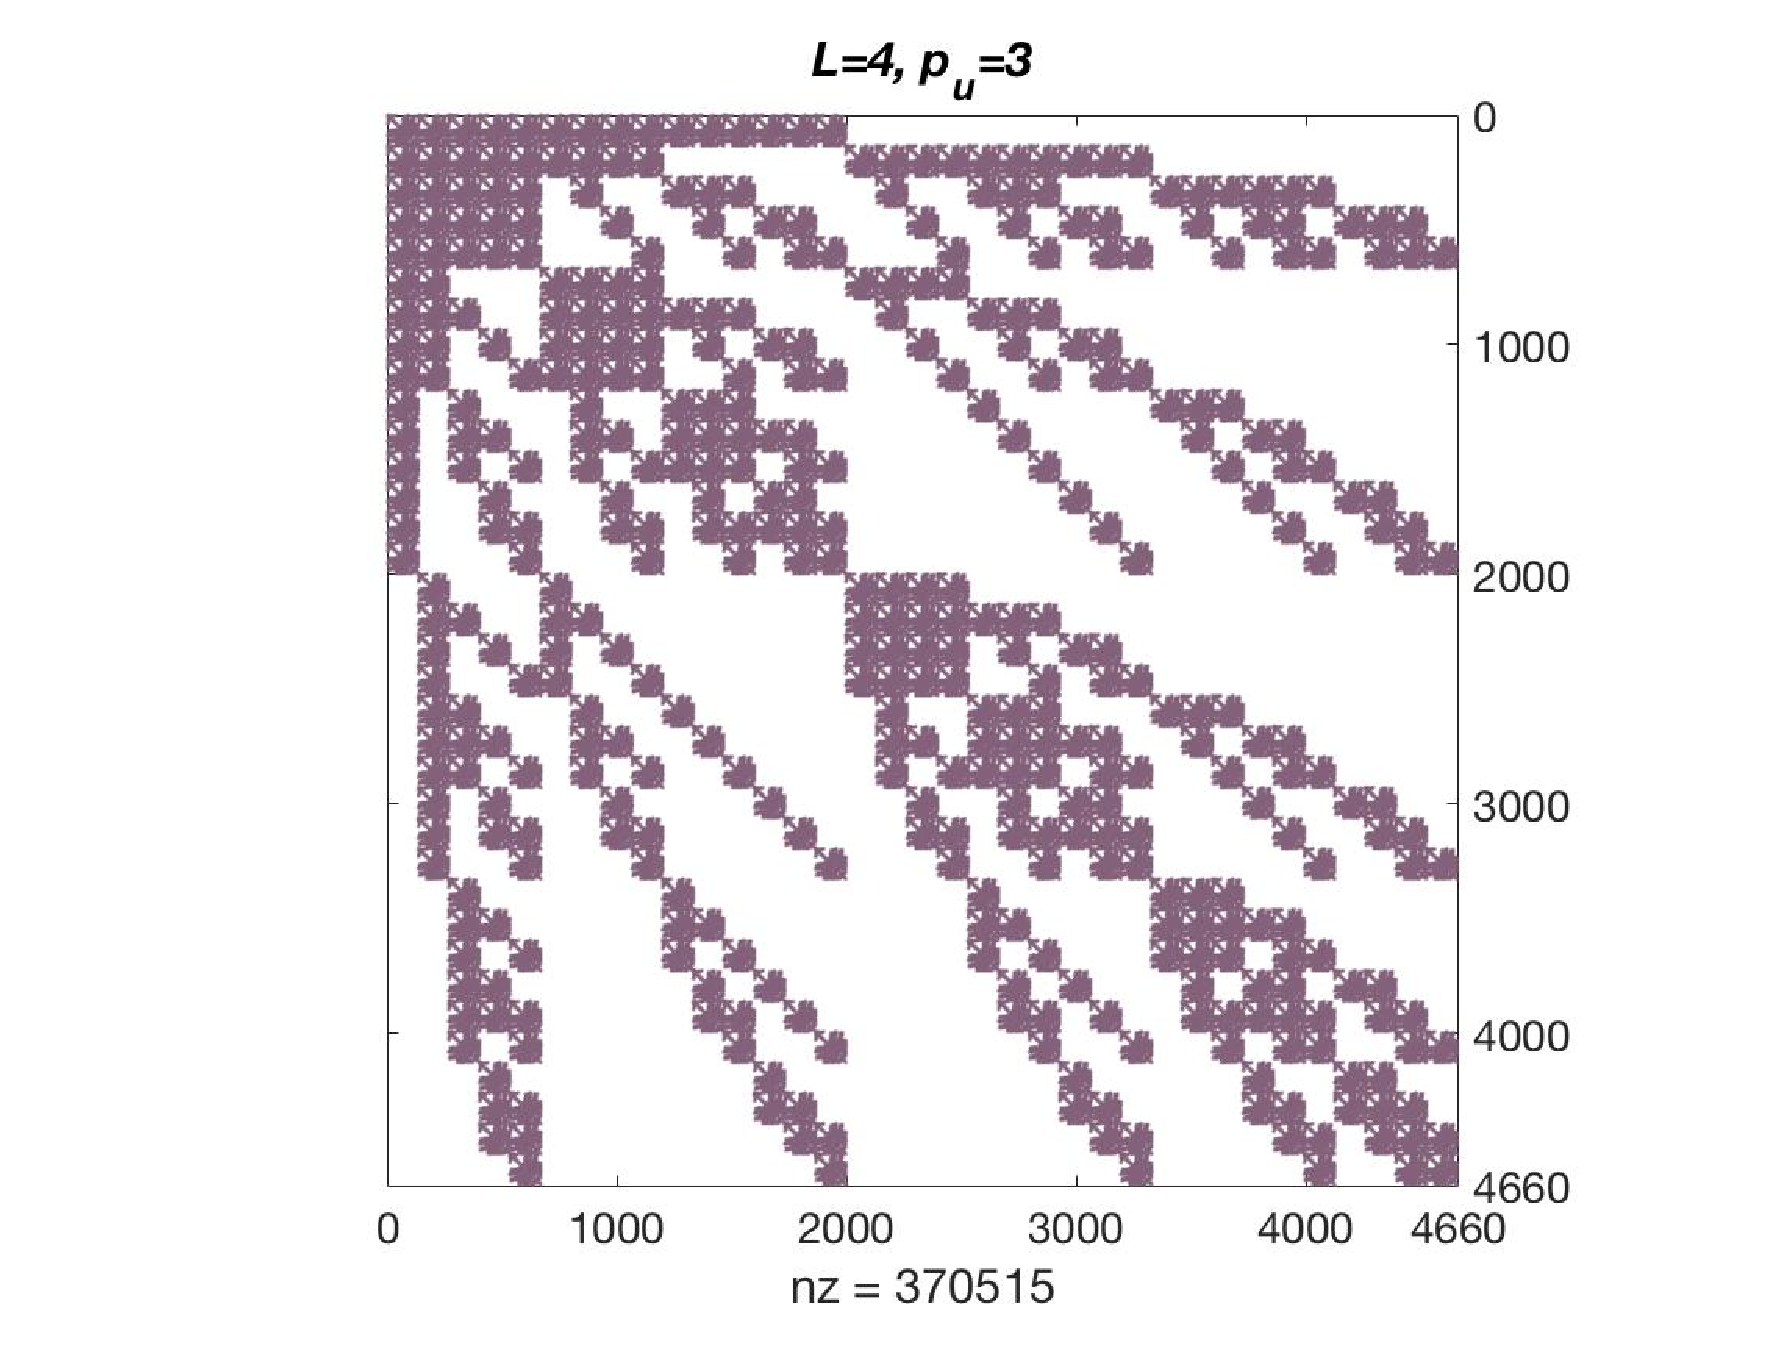
\includegraphics[width=0.49\textwidth,height=0.26\textheight]{plots/L4p3.eps}
 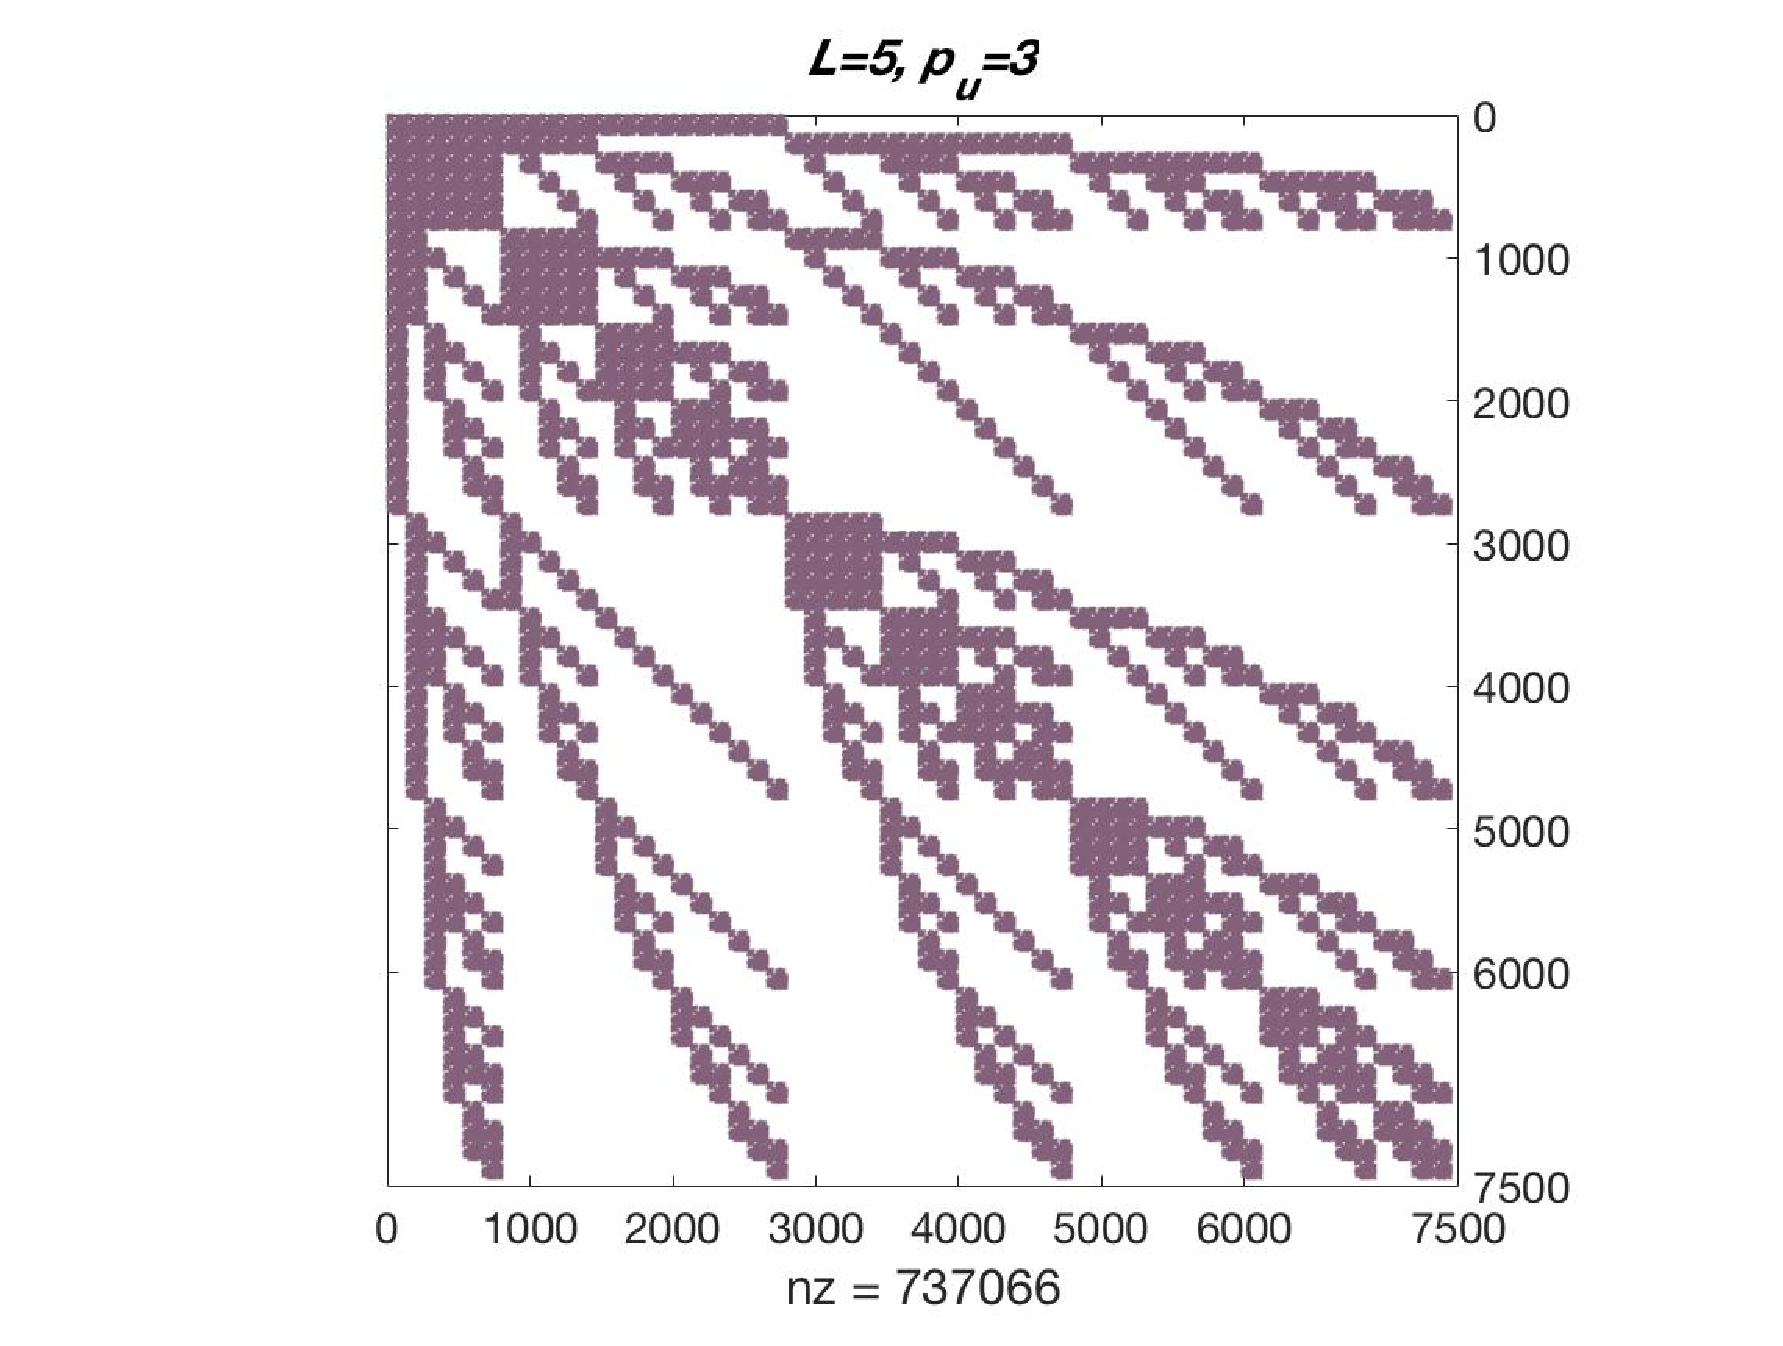
\includegraphics[width=0.49\textwidth,height=0.26\textheight]{plots/L5p3.eps}
 \caption{Block-sparse structures of the intrusive system matrices for a fixed mesh resolution with $p_{u}=3$ and $L=4,5$}
 \label{fig:sFEMdim}
\end{figure}
%-----------------------------------------------------
In \Cref{fig:sFEMord} and \ref{fig:sFEMdim}, the block-diagonal structures of intrusive system matrices are presented. In \Cref{fig:sFEMord}, $p_{u}$ is increased from $4$ to $5$ while keeping $L=3$ fixed. In \Cref{fig:sFEMdim}, $L$ is increased from $4$ to $5$
while keeping $p_{u}=3$ fixed.

Note that the effect of increasing the order of expansion is different from that of the number of random variables.
The system matrix resulting from varying $L$ have more nonzero entries compared to the one resulting from a similar change in $p_u$ as indicated by the number of nonzero entries $nz$ in~\Cref{fig:sFEMord} and \ref{fig:sFEMdim}.
For example, with $L=5$ and $p_u=3$ we have $0.73$ million nonzero elements compared to $L=3$ and $p_u=5$ which has $0.60$ million nonzero elements. Therefore, an increase in the number of random variables may pose a more significant challenge compared to increasing order of expansion or the finite element mesh resolution concerning memory and computation requirements.  However, both the order $p_u$ and dimension $L$ influence the size and structure of the stochastic assembly matrix, thereby, affecting the condition number of the system matrix~\cite{ghanem1996numerical,pellissetti2000iterative}.


To compare the performances of the intrusive approach with the non-intrusive approach, we consider the four different cases by selecting the number of random variables $L$ as 2, 3, 4 and 5. The second order PCE is used for input PCE ensuring non-Gaussian terms are included in the series expansion. The order of the input PCE is kept constant for all the experiments.
%Note that the order of input PCE $p_{A}$ is kept constant for all the experiments and primary attention is given to the number of random variables $L$.
The minimum order of PCE used in the expansion of solution process is $p_{u} = 3$ which is higher than input PCE order, which captures the non-Gaussian effects~\cite{ghanem1999ingredients,ghanem1999stochastic}. Then $p_{u}$ is varied as 3, 4 and 5 to perform error analysis in the lower order PCE coefficients.

Note that the intrusive SSFEM code employed for all the simulation in this exercise is validated with the SSFEM code developed by Khalil~\cite{khalil2013bayesian}, which is validated using method of manufactured solution (see Appendix-D.3 in~\cite{khalil2013bayesian} for more details). Additionally, the intrusive SSFEM serial solver used here is validated with the parallel domain decomposition based solver employed in~\cite{desai2017scalable} %\Cref{chap:ddm2d},
which is validated against MCS in~\cite{desai2019scalable}. %\Cref{apn:validation}.
For non-intrusive case, the deterministic samples are simulated using the
code validated against an analytical case in FEniCS/puffin~\cite{logg2012FEniCS,aloggs2013puffin}. The correctness of the quadrature points used to solve the integrals (in the numerator and the denominator of~\Cref{eq:NISPpce}) in the NISP approach are validated with the exact solution available for the ${\left<{\Psi_k^2({\pmb{\xi}})}  \right>}$. %~\Cref{apn:validation}

The relative error norms are computed using $p_{u} = 6$ in the intrusive SSFEM and used as the reference solution. For instance, the relative error in the $i^{th}$ order solution coefficient can be computed as $||({\mathrm{\hat{\bf{u}}}^{i}_{p_{u}=j}} -{\mathrm{\hat{\bf{u}}}^{i}_{p_{u}=6}} )|| /||{\mathrm{\hat{\bf{u}}}^{i}_{p_{u}=6}}||$
with $j=3,4$ and $5$ where $||.||$ denotes $\mathrm{L_2}$ norm. For each case, the simulation is restricted to the maximum order of $p_{u}= 6$. This is because we were not able to fit the system matrix for the intrusive approach for the higher-order cases (i.e., $p_{u} > 6$) in the computer with quad-core processor and $16$ gigabytes (GB) of random access memory (RAM) used for all the simulations.

The relative error norms in $0^{th}, 1^{st}$ and $2^{nd}$ order solution coefficients with $L=2, 3, 4$ and $5$ for both intrusive and non-intrusive SSFEM are plotted in \Crefrange{fig:2RV}{fig:5RV}. % respectively.
In the intrusive approach, as the order of expansion of the solution process $p_{u}$ increases, the relative error in the lower order solution coefficients decreases. For example, if $p_u$ increased from 3 to 4, the error in the lower order expansion terms, i.e., for $p_u=$ 0, 1 or 2, decreases as expected.
Similarly in the non-intrusive approach, as the level of quadrature $l$ increases, the relative error in the individual solution PCE coefficients decreases. Note that, in the non-intrusive approach the solution coefficients are independent of each other as opposed to the intrusive approach, where the error in the lower order solution coefficients decrease as we include the higher-order expansion terms.

For the cases with lower order solution coefficients and a few random variables, for instance, $0^{th}$ order with $L=2$ presented in \Cref{fig:2RV}, the relative errors are similar in both intrusive and non-intrusive approaches with $l=p_{u}$.
For the higher-order solution coefficients with a large number of random variables, for instance, the $3^{rd}$ order coefficient with $L=3$ presented in \Cref{fig:3RV},
%For a fixed order of intrusive and fixed level in non-intrusive, for instance $p_{u}=3$ and $l=3$,
%For the third order, $p_{u} =3$ in intrusive and third level, $l=3$ in non-intrusive,
the relative error is less in the case of intrusive approach compared to non-intrusive approach for $p_{u} = l$. The difference between the relative errors for the intrusive and non-intrusive approach grows as the $p_{u}$ and the $L$ increases. Therefore, in order to achieve the same level of accuracy in the PCE coefficients of the solution process, we need a higher level of the sparse quadrature in non-intrusive approach compared to the order of expansion in the intrusive approach (i.e., $l > p_{u}$).
For example, in the case of $1^{st}$ order solution coefficient with $4$ random variables presented in \Cref{fig:4RV}, to achieve the same level of accuracy as intrusive approach with $p_{u}=3$, we need the fourth level of quadrature. Similarly, in the case of $2^{nd}$ order solution coefficient with $5$ random variables shown in \Cref{fig:5RV}, to achieve the same level of accuracy as in intrusive approach with $p_{u}=3$, we need the fifth level of quadrature. % or higher level of quadrature.


%-------------ABhi commented--------------

\begin{figure}[htbp]
\centering
 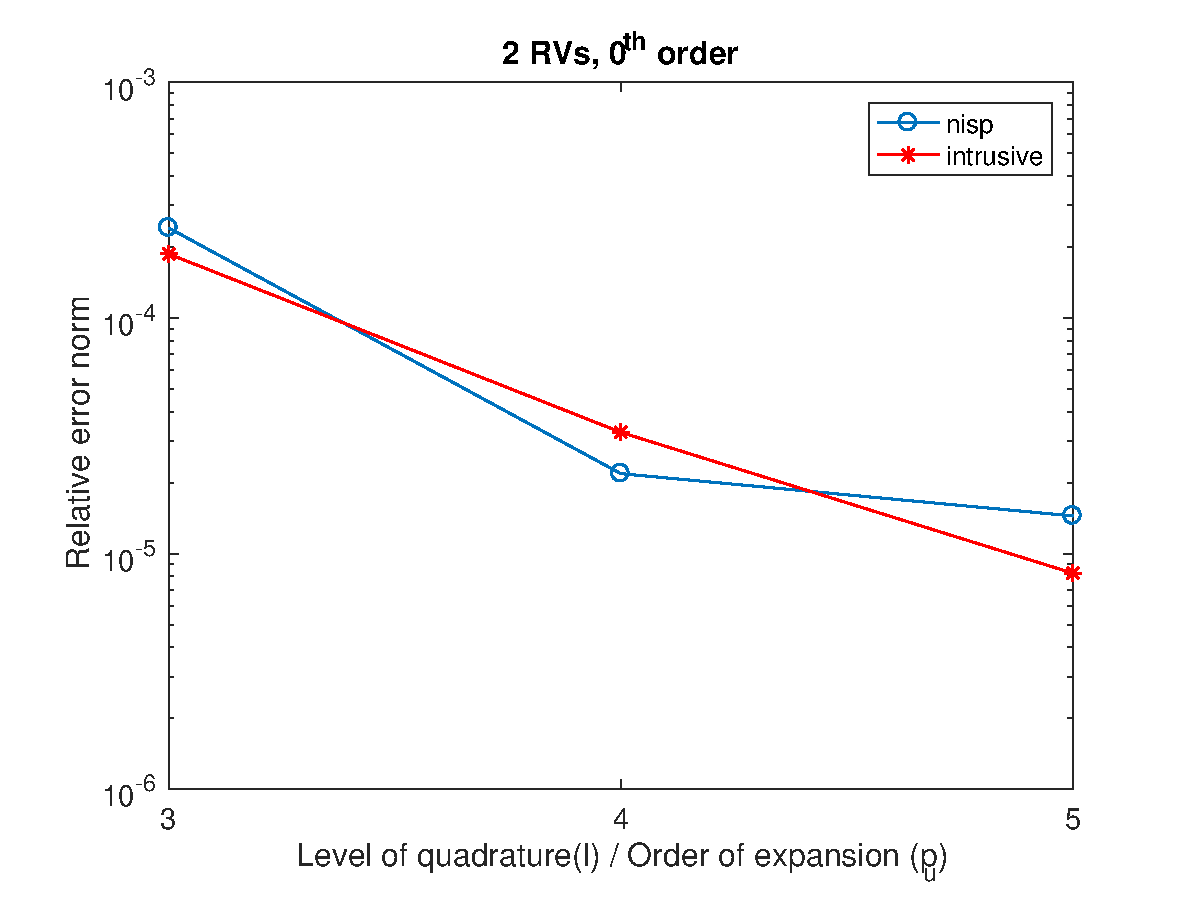
\includegraphics[width=0.32\textwidth,height=0.18\textheight]{plots/sigma04_2RN_u0_order0.eps}
 \includegraphics[width=0.32\textwidth,height=0.18\textheight]{plots/sigma04_2RN_u2_order1.eps}
 \includegraphics[width=0.32\textwidth,height=0.18\textheight]{plots/sigma04_2RN_u4_order2.eps}
 \caption{Error norms in $0^{th}, 1^{st}$ and $2^{nd}$ order PCE coefficients for $L=2$.}
 \label{fig:2RV}
\end{figure}
\begin{figure}[htbp]
\centering
 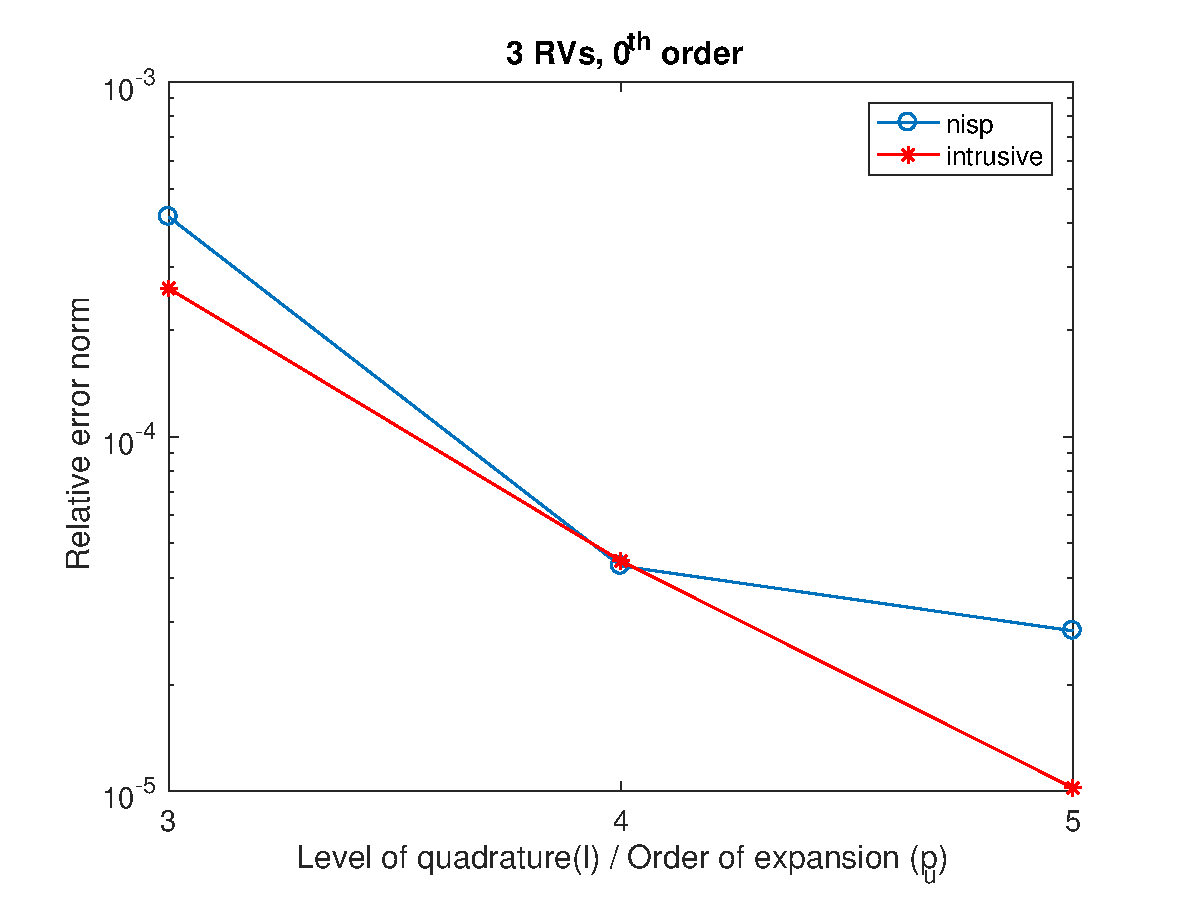
\includegraphics[width=0.32\textwidth,height=0.18\textheight]{plots/sigma04_3RN_u0_order0.eps}
 \includegraphics[width=0.32\textwidth,height=0.18\textheight]{plots/sigma04_3RN_u1_order1.eps}
 \includegraphics[width=0.32\textwidth,height=0.18\textheight]{plots/sigma04_3RN_u4_order2.eps}
 \caption{Error norms in $0^{th}, 1^{st}$ and $2^{nd}$ order PCE coefficients for $L=3$.}
 \label{fig:3RV}
\end{figure}
\begin{figure}[htbp]
\centering
 \includegraphics[width=0.32\textwidth,height=0.18\textheight]{plots/sigma04_4RN_u0_order0.eps}
 \includegraphics[width=0.32\textwidth,height=0.18\textheight]{plots/sigma04_4RN_u1_order1.eps}
 \includegraphics[width=0.32\textwidth,height=0.18\textheight]{plots/sigma04_4RN_u7_order2.eps}
 \caption{Error norms in $0^{th}, 1^{st}$ and $2^{nd}$ order PCE coefficients for $L=4$.}
 \label{fig:4RV}
\end{figure}
\begin{figure}[htbp]
\centering
 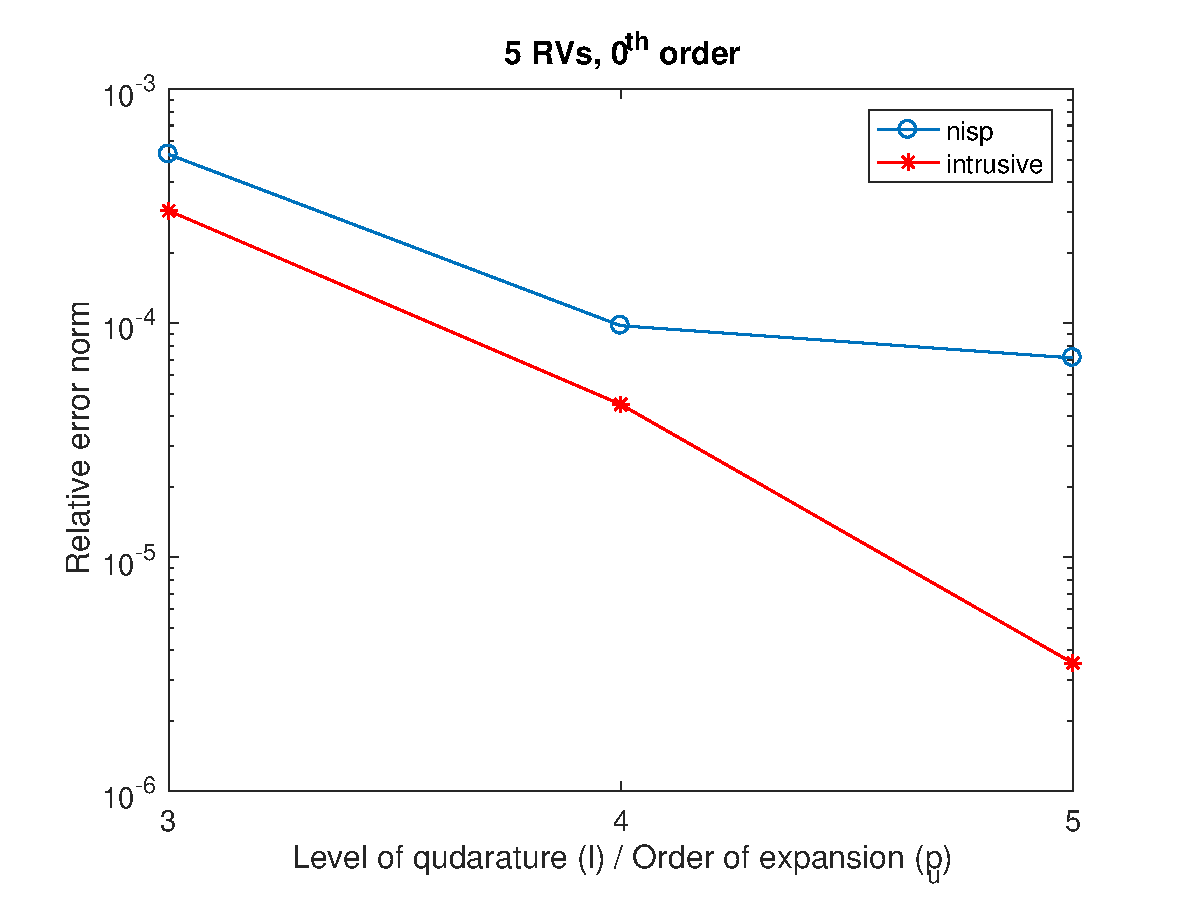
\includegraphics[width=0.32\textwidth,height=0.18\textheight]{plots/sigma04_5RN_u0_order0.eps}
 \includegraphics[width=0.32\textwidth,height=0.18\textheight]{plots/sigma04_5RN_u3_order1.eps}
 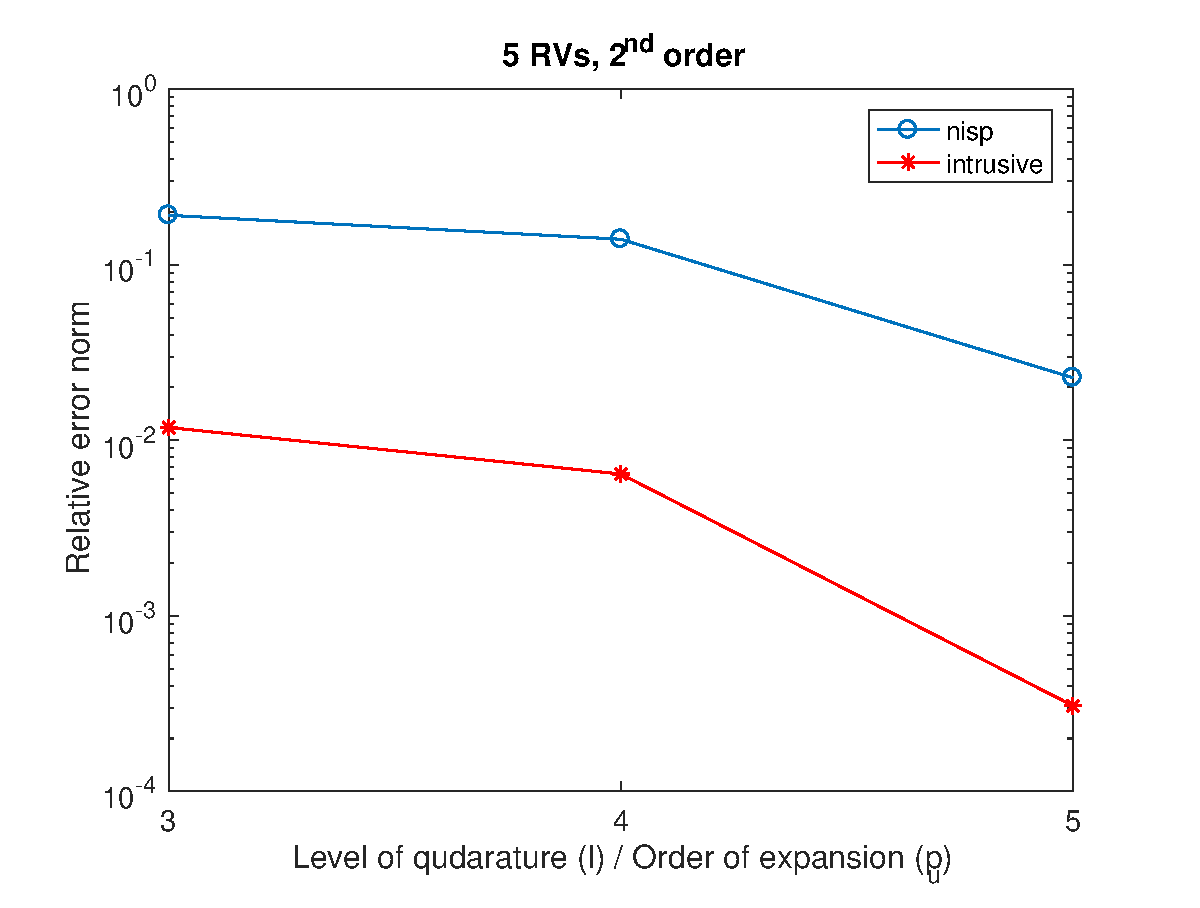
\includegraphics[width=0.32\textwidth,height=0.18\textheight]{plots/sigma04_5RN_u12_order2.eps}
 \caption{Comparison of relative error norms between intrusive and non-intrusive SSFEM in $0^{th}, 1^{st}$ and $2^{nd}$ order PCE coefficients for $L=5$.}
 \label{fig:5RV}
\end{figure}


\begin{figure}[htbp]
\centering
 \includegraphics[width=0.49\textwidth,height=0.3\textheight]{plots/sigma04_2RN_sd.eps}
 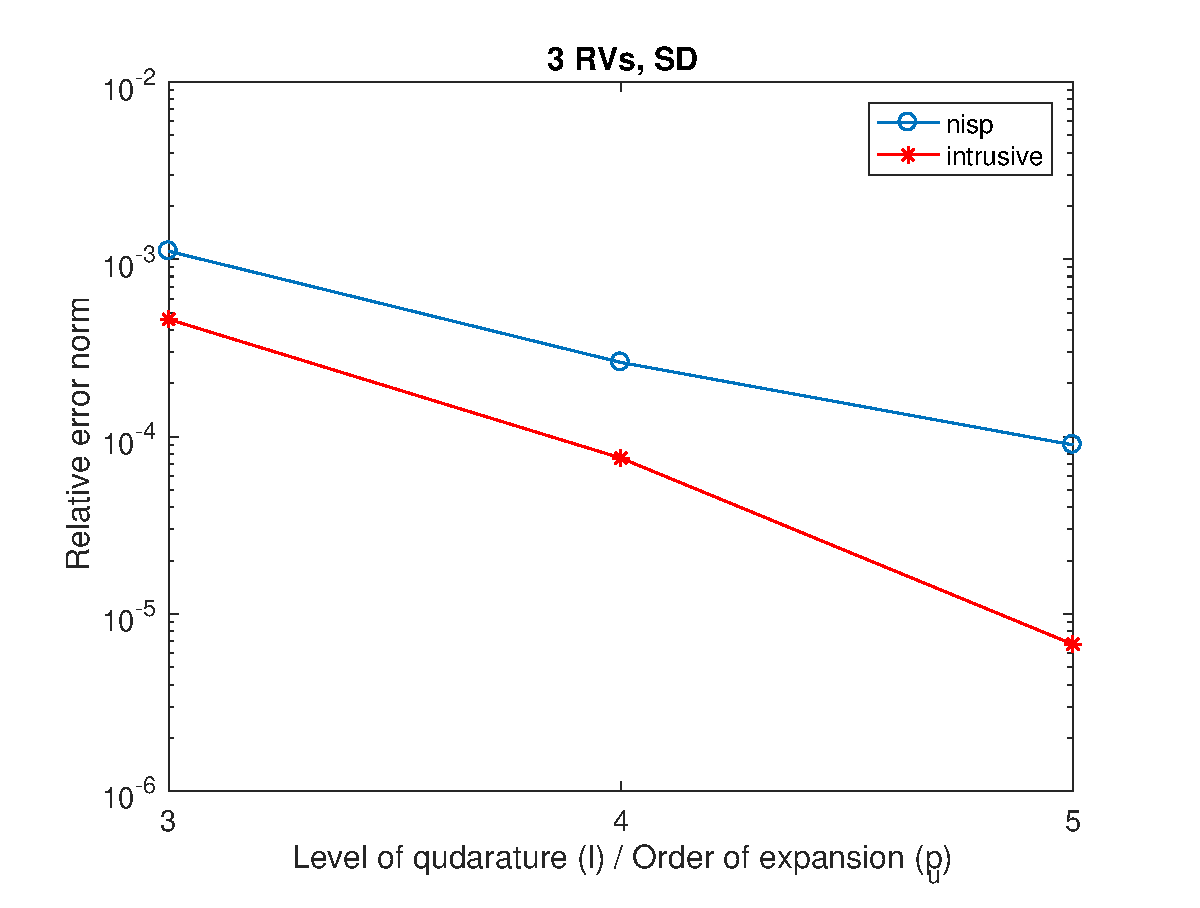
\includegraphics[width=0.49\textwidth,height=0.3\textheight]{plots/sigma04_3RN_sd.eps}

\

\

 \includegraphics[width=0.49\textwidth,height=0.3\textheight]{plots/sigma04_4RN_sd.eps}
 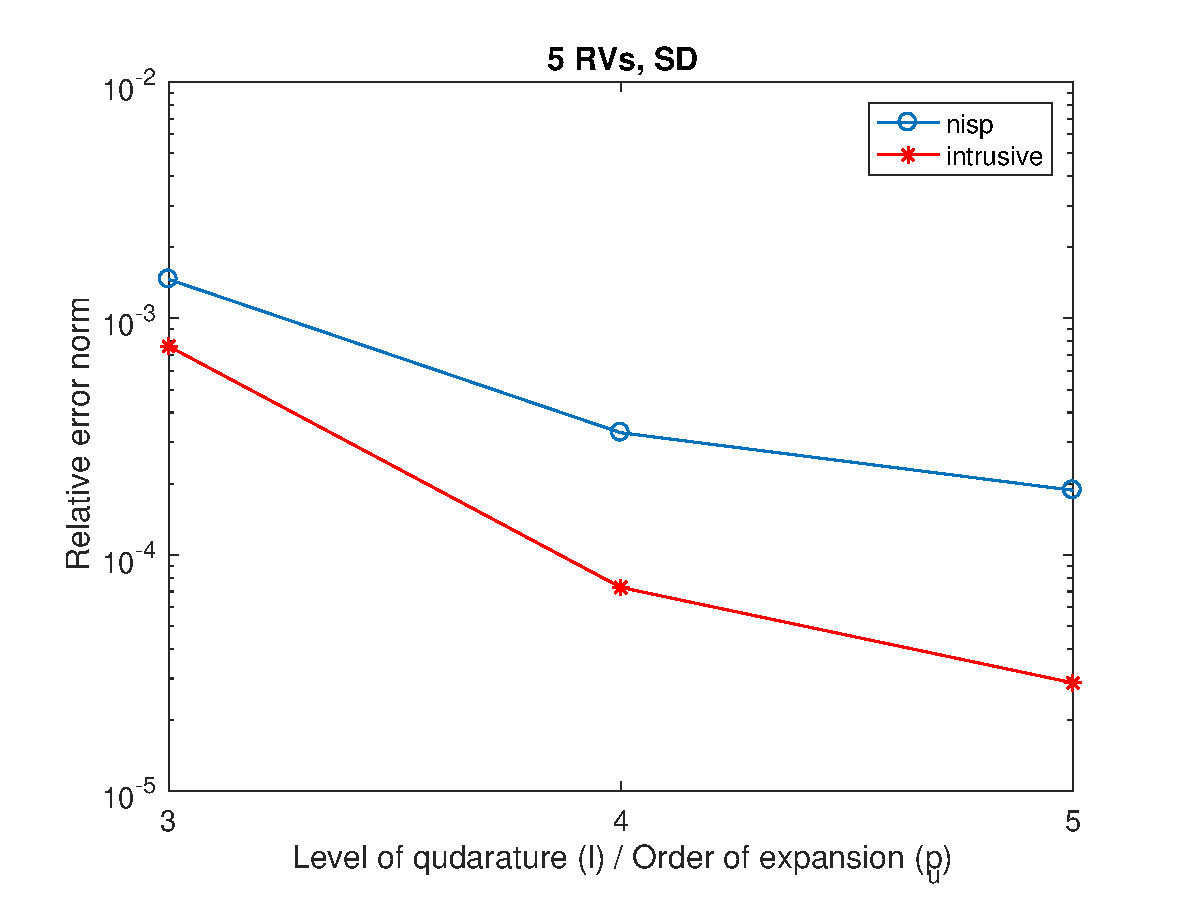
\includegraphics[width=0.49\textwidth,height=0.3\textheight]{plots/sigma04_5RN_sd.eps}
 \caption{Comparison of relative error norms between intrusive and non-intrusive SSFEM in the standard deviation (computed for all nodes) of the solution process for $L=2,3,4$ and $5$.}
 \label{fig:SD}
\end{figure}

%----------------------------------------
For the same cases discussed above, the relative error norms in the standard deviation $\sigma_u$ of the solution process (for all nodes) %(which is a function of solution coefficients)  %, i.e., $L=2, 3, 4$ and $5$, for both intrusive and non-intrusive SSFEM approach
are shown in~\Cref{fig:SD}.
%The standard deviation $\sigma^d_u$ at the node $d$ is computed as \textcolor{red}{$\sigma^d_u = \sqrt(\sum_{i=0}^{P_u} (u^d_i)^2 \Psi^2_i)$}.
Also, for $L=4$ the error surface plots in the SD of the solution process using intrusive with $p_u=3,4$ and $5$ and NISP with $l=3,4$ and $5$ are compared in~\Cref{fig:SD_errorSurf}.
These plots also suggest that, for the same level of accuracy in the standard deviation of the solution process with the intrusive SSFEM approach, we need a higher level of quadrature to solve the integral involved in the non-intrusive approach.
Therefore, to model the uncertainty as a non-Gaussian stochastic process characterized by a large number of random variables we have to use the higher level sparse grid quadrature, i.e., $l>>p_u$.
Consequently, we need a large number of samples in the non-intrusive approach. For instance, if we increase the level of quadrature from $3$ to $4$ or $5$, there is a small increase in the number of quadrature points for low-dimensional cases, for example $L=5$. However, the number of samples for high-dimensional cases, for example $L=15$, increases quickly compared to the low-dimensional cases (i.e., $L=5$) as shown in~\Cref{table:table3}.
\begin{table}[htbp]
\centering
\begin{tabular}{l*{6}{c}r}
%\multicolumn{1}{ c }{} & \multicolumn{6}{ c }{$N_{s}$}
\hline
$N_s$              & $L=5$  \ \ \ \ \ & $L=15$ \\
\hline
$l=3$	& \ 241 & \ 11561  \\ \hline
$l=4$ & \ 781 & \ 120401  \\ \hline
$l=5$ & \ 2203 & \ 259607  \\
\hline
\end{tabular}
\caption{Number of sample (quadrature) points $N_s$ in the sparse grid with level $l$ and the number of random variables $L$.}
\label{table:table3}
\end{table}

%---------------abhi commented --------------
\begin{figure}[htbp]
\centering
 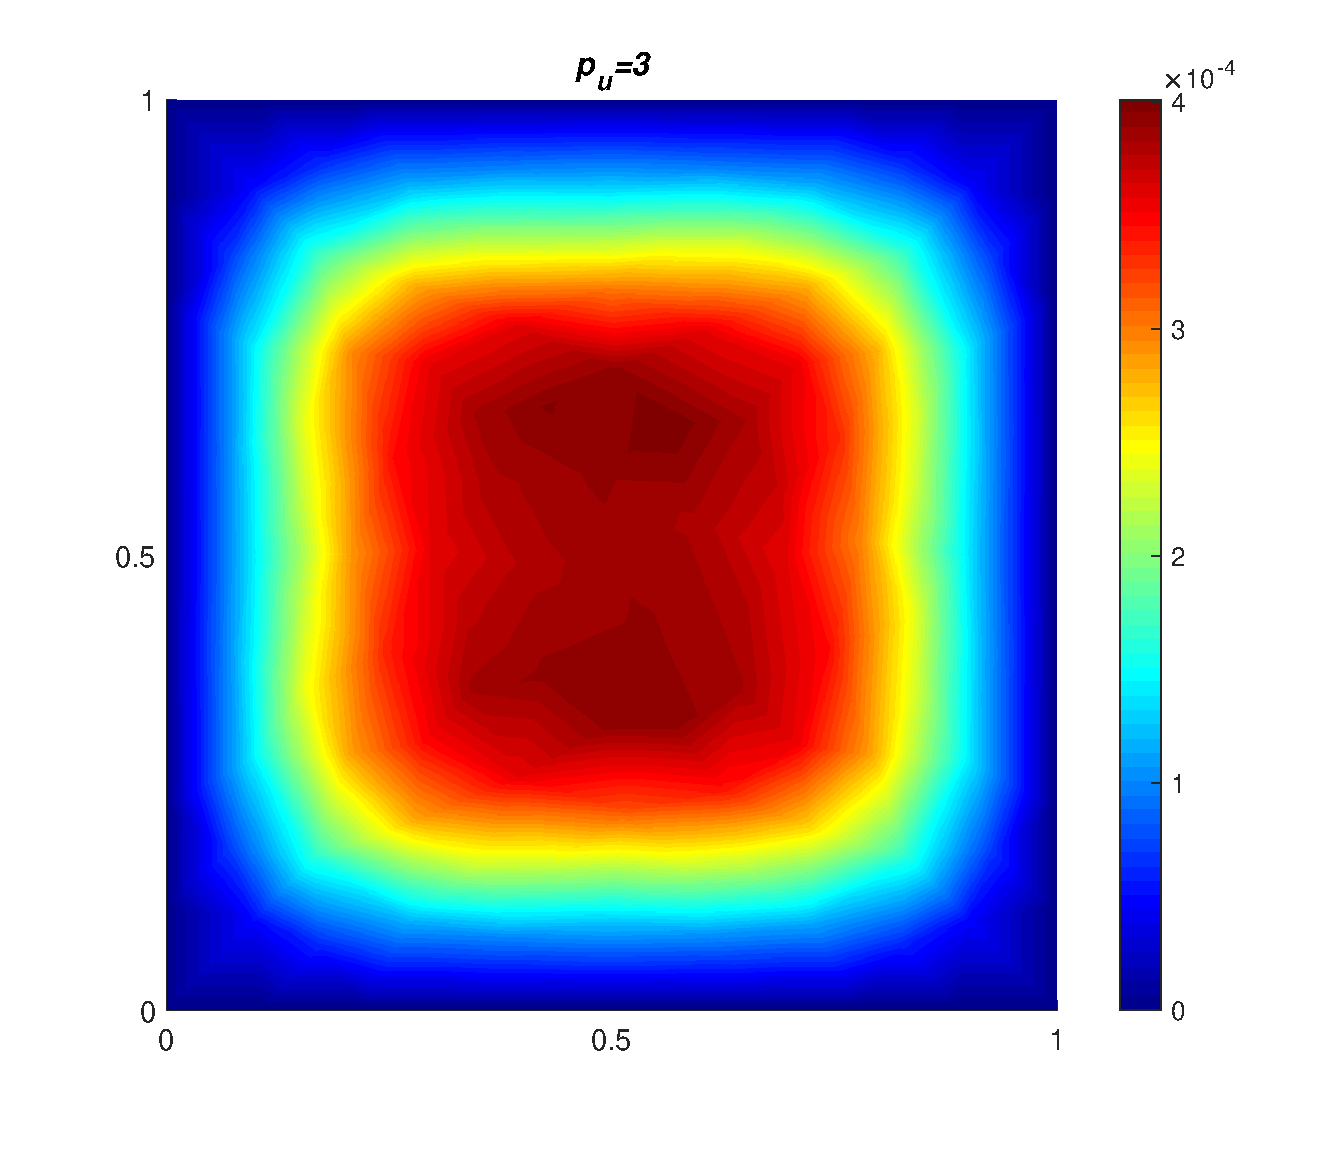
\includegraphics[width=0.45\textwidth,height=0.27\textheight]{plots/errorSurf_L4p3.eps}
 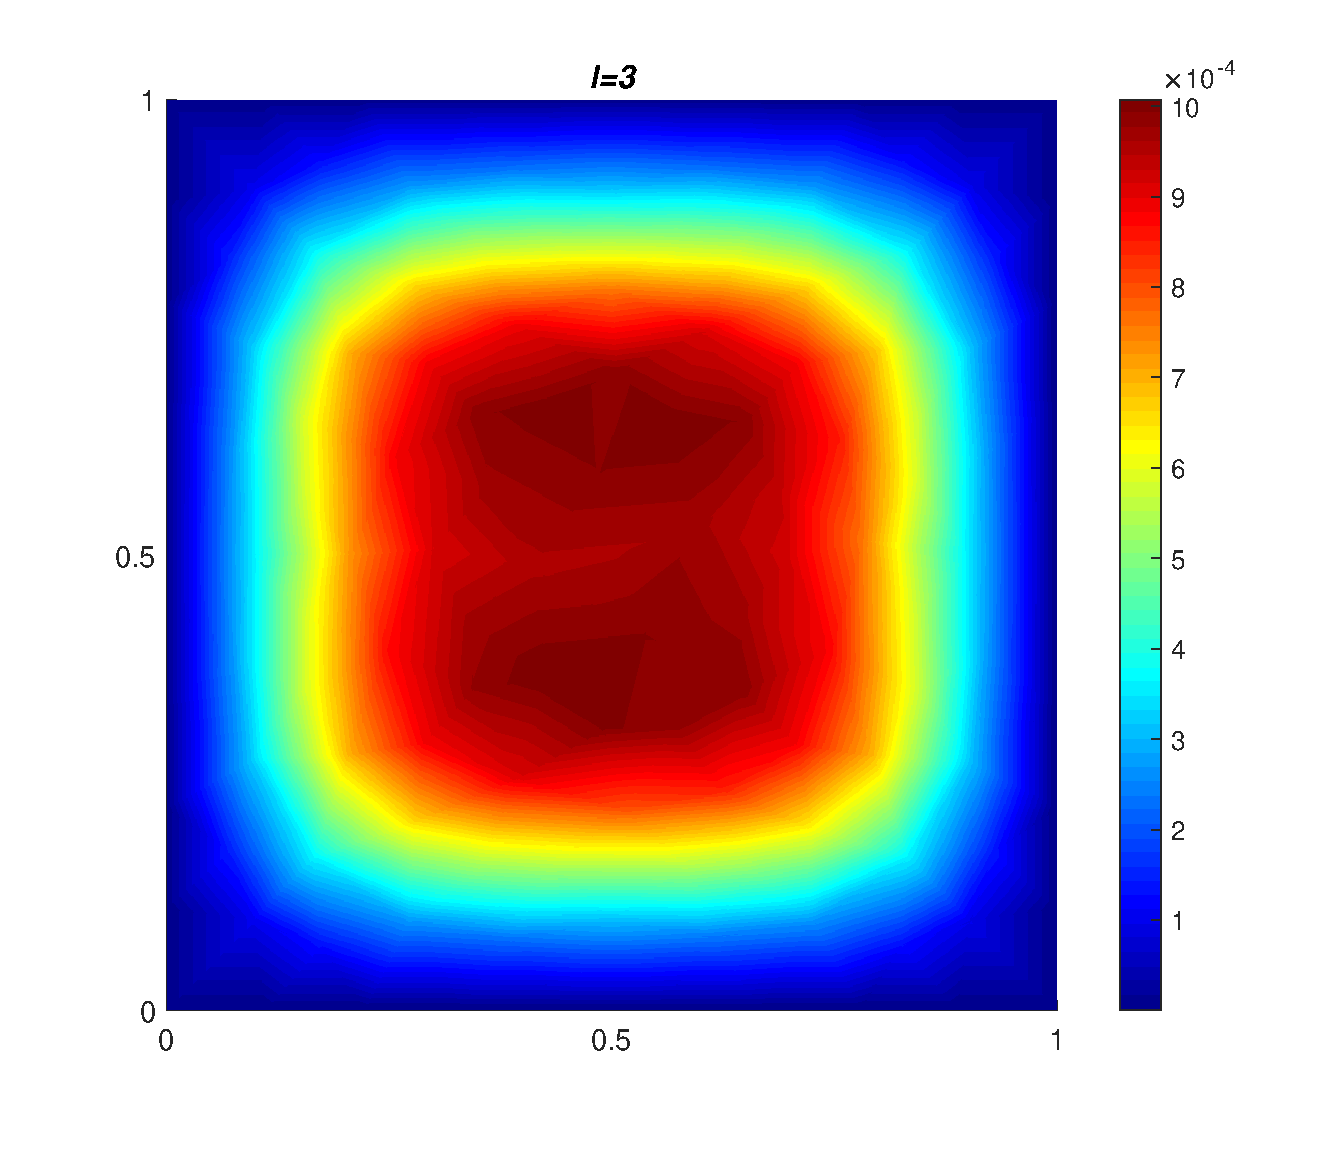
\includegraphics[width=0.45\textwidth,height=0.27\textheight]{plots/errorSurf_L4l3.eps}

 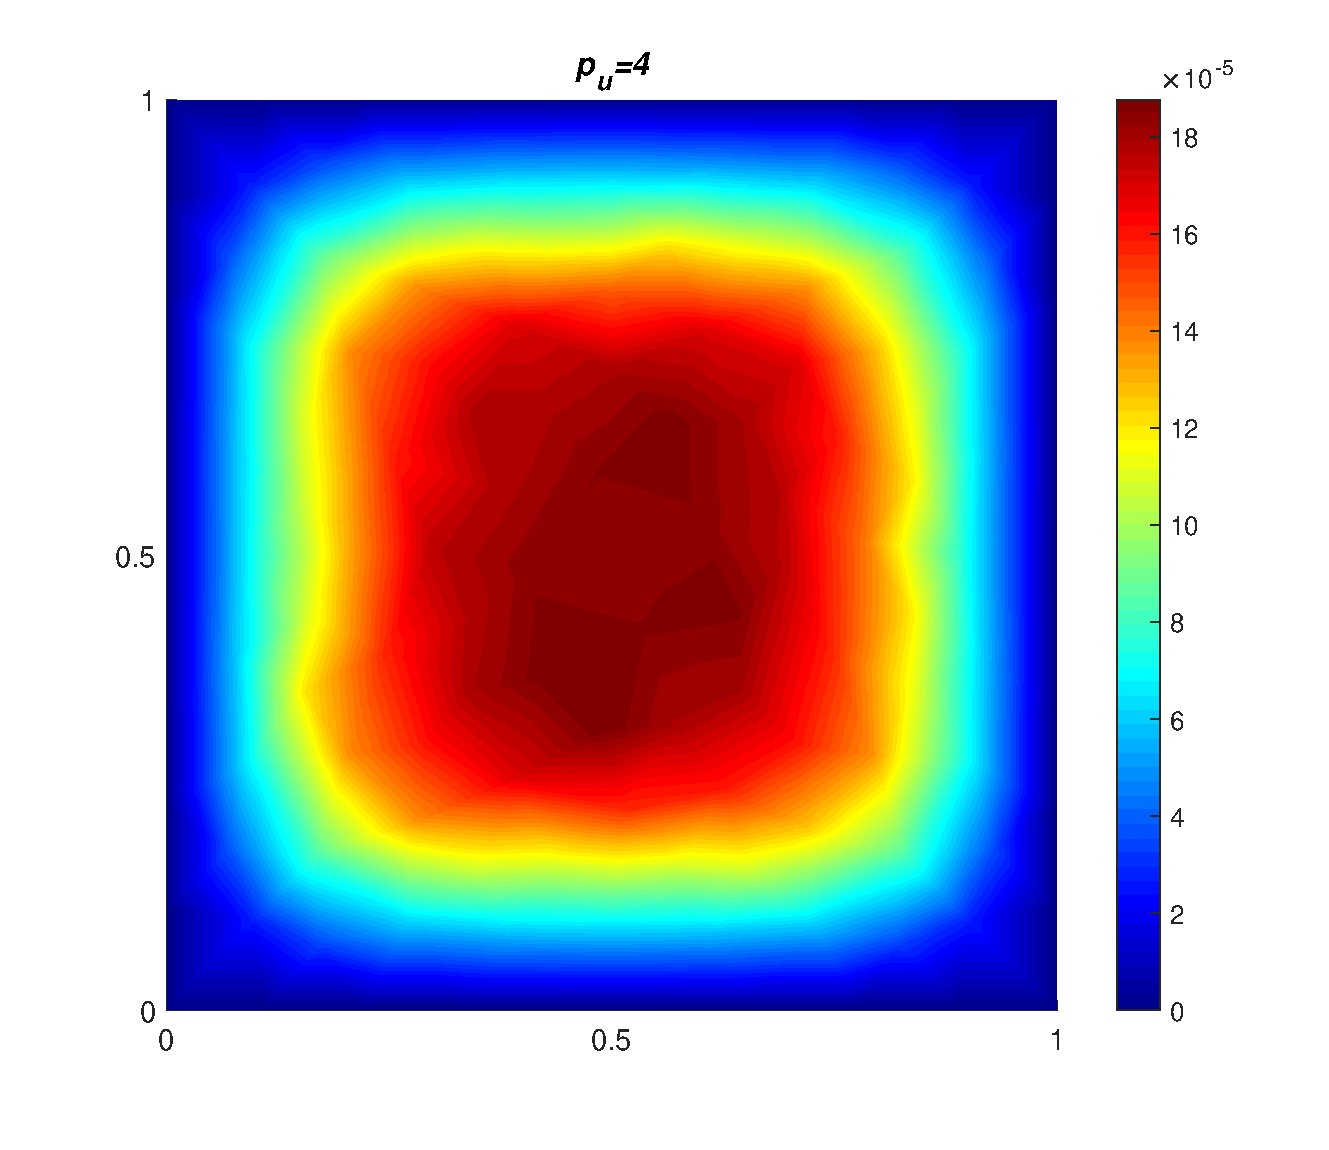
\includegraphics[width=0.45\textwidth,height=0.27\textheight]{plots/errorSurf_L4p4.eps}
 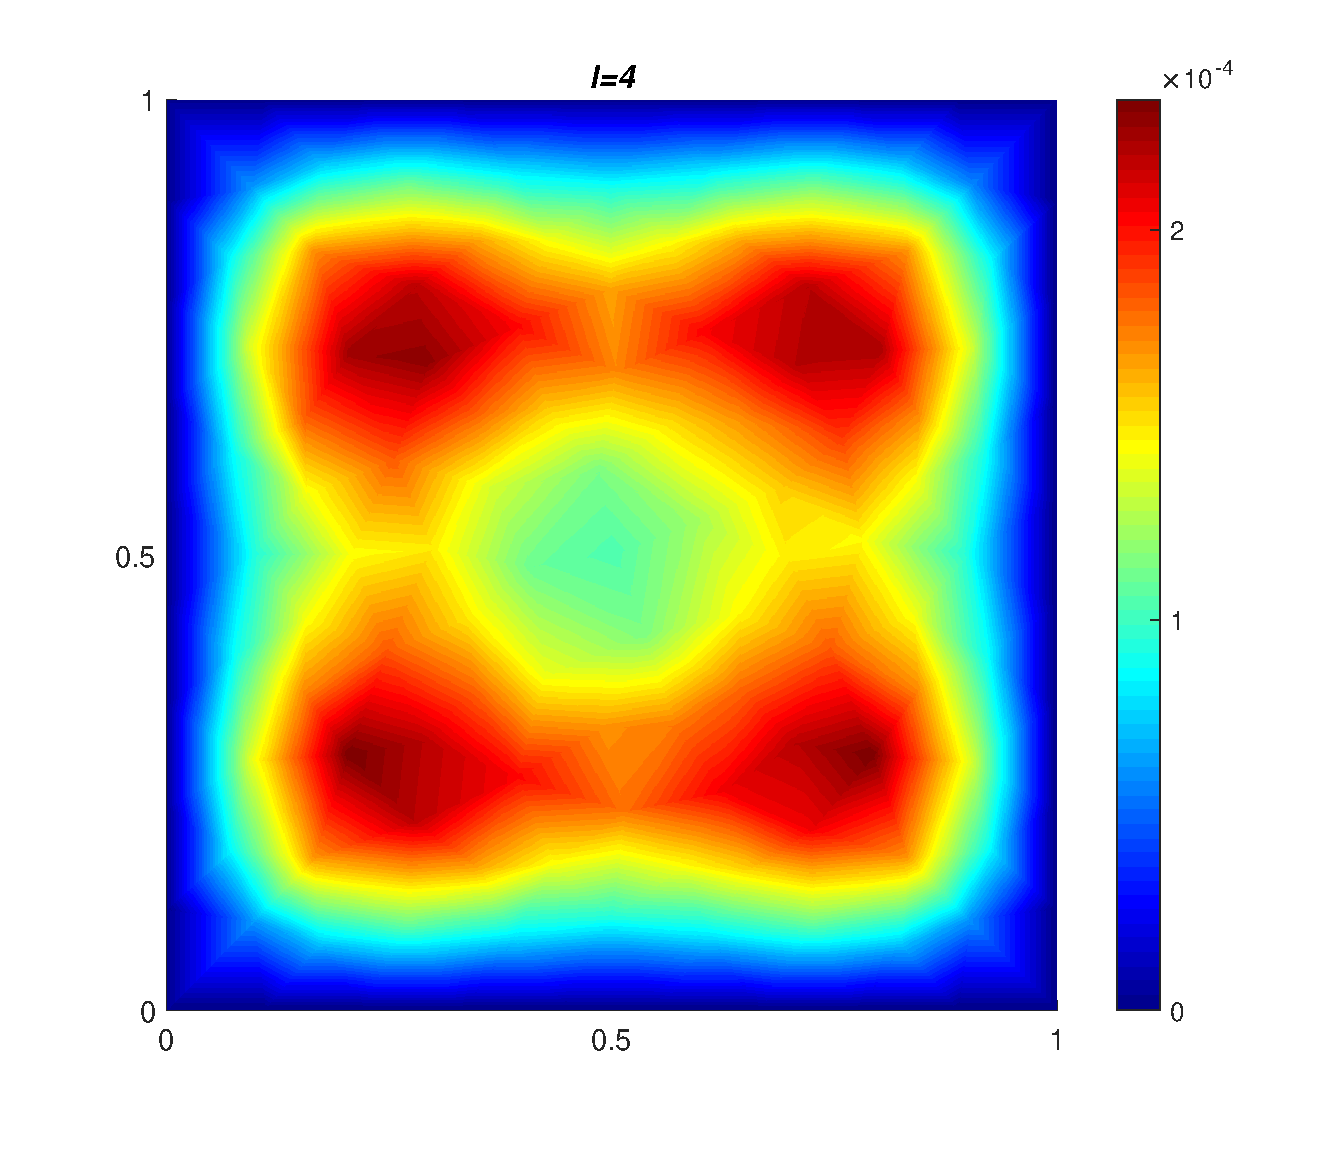
\includegraphics[width=0.45\textwidth,height=0.27\textheight]{plots/errorSurf_L4l4.eps}

 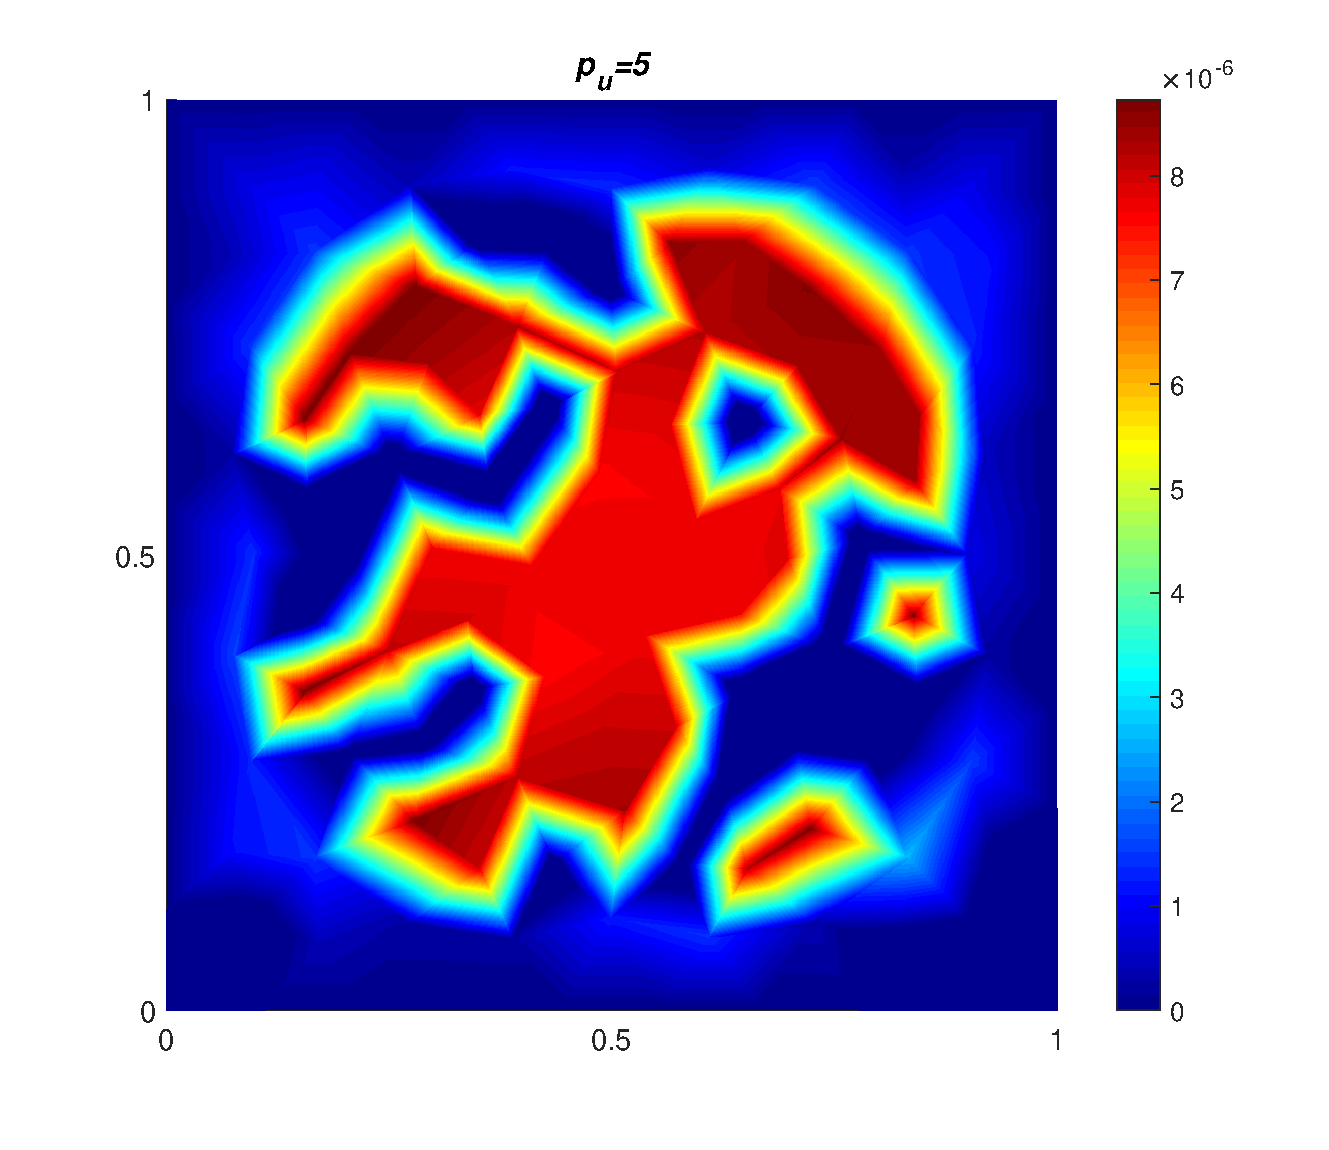
\includegraphics[width=0.45\textwidth,height=0.27\textheight]{plots/errorSurf_L4p5.eps}
 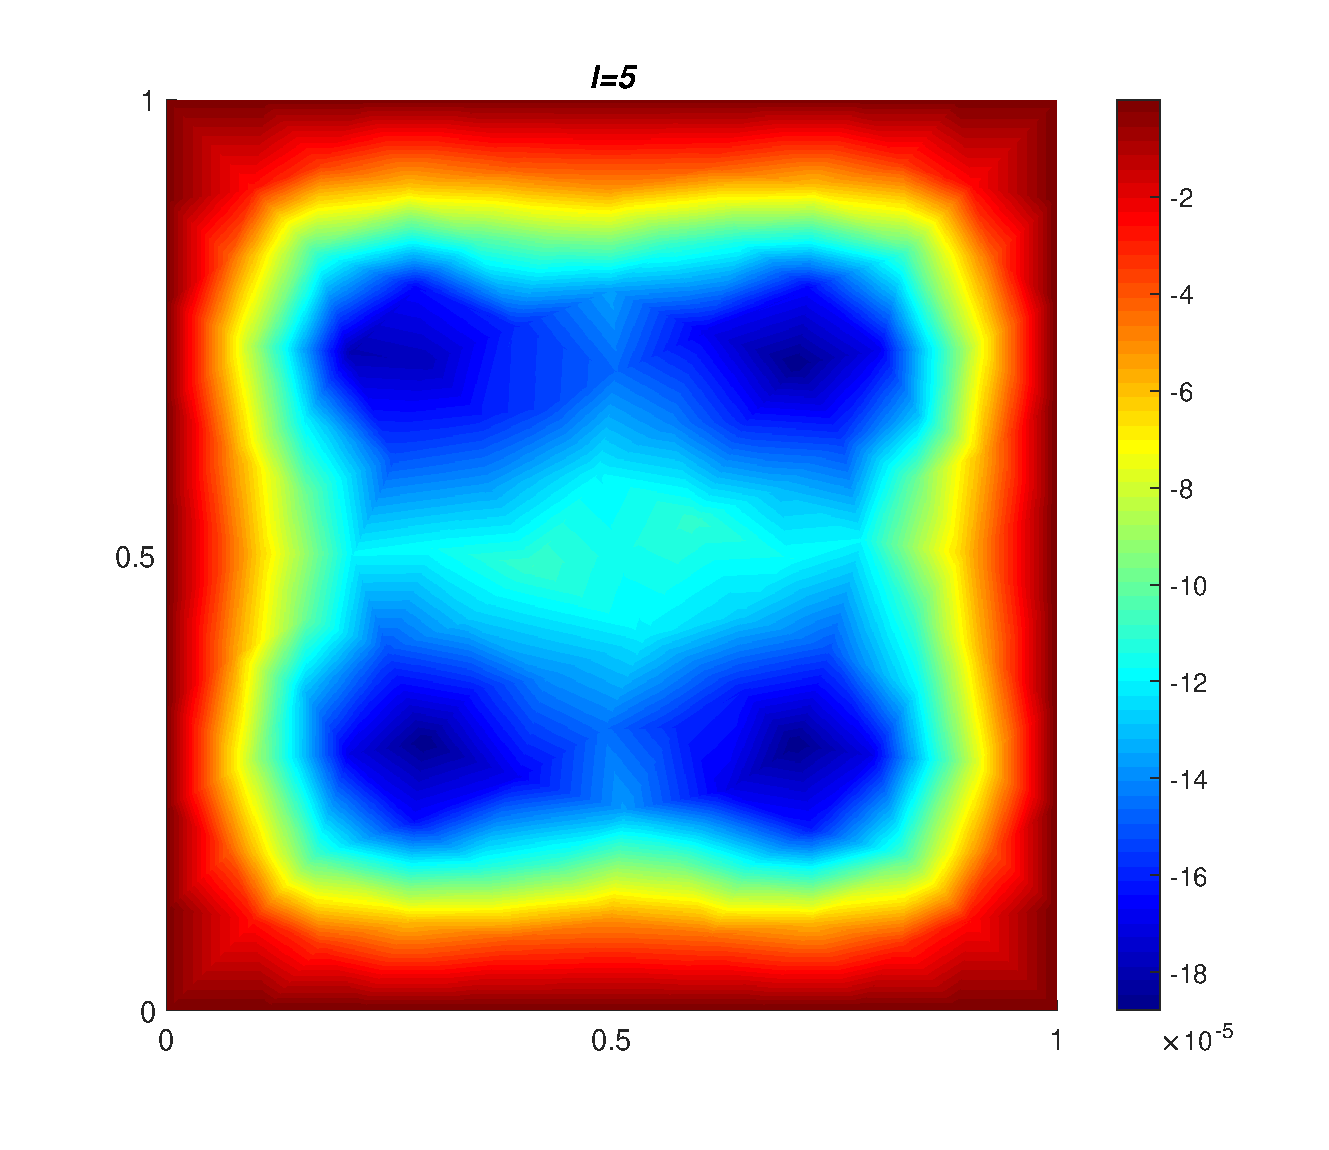
\includegraphics[width=0.45\textwidth,height=0.27\textheight]{plots/errorSurf_L4l5.eps}

  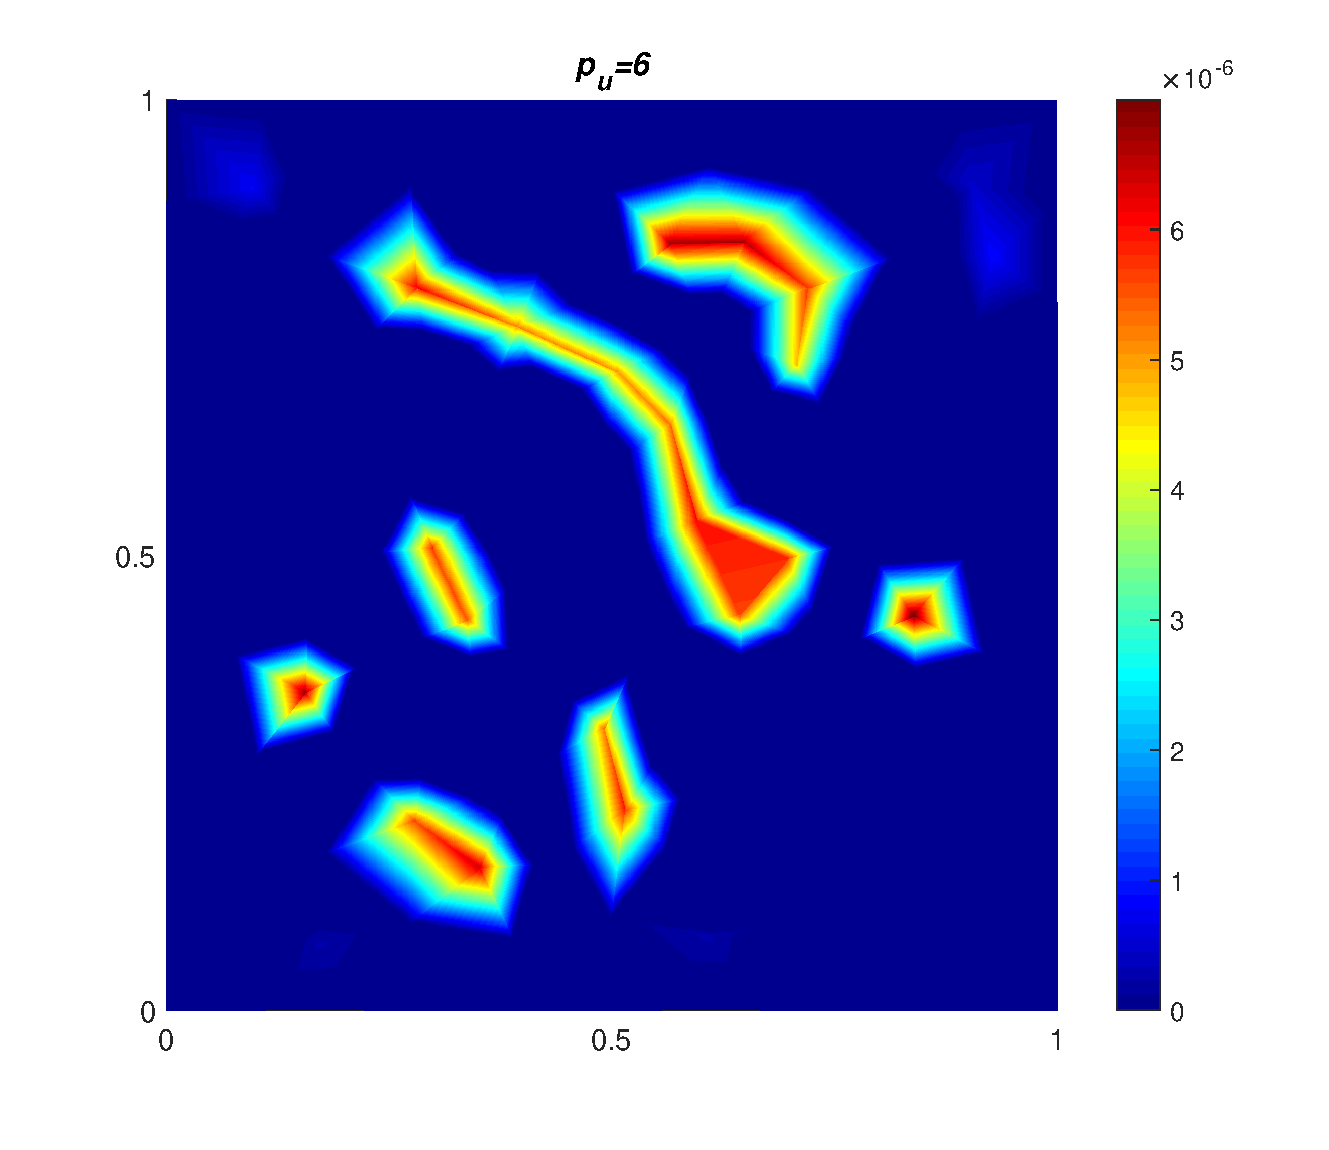
\includegraphics[width=0.42\textwidth,height=0.24\textheight]{plots/errorSurf_L4p6.eps}
  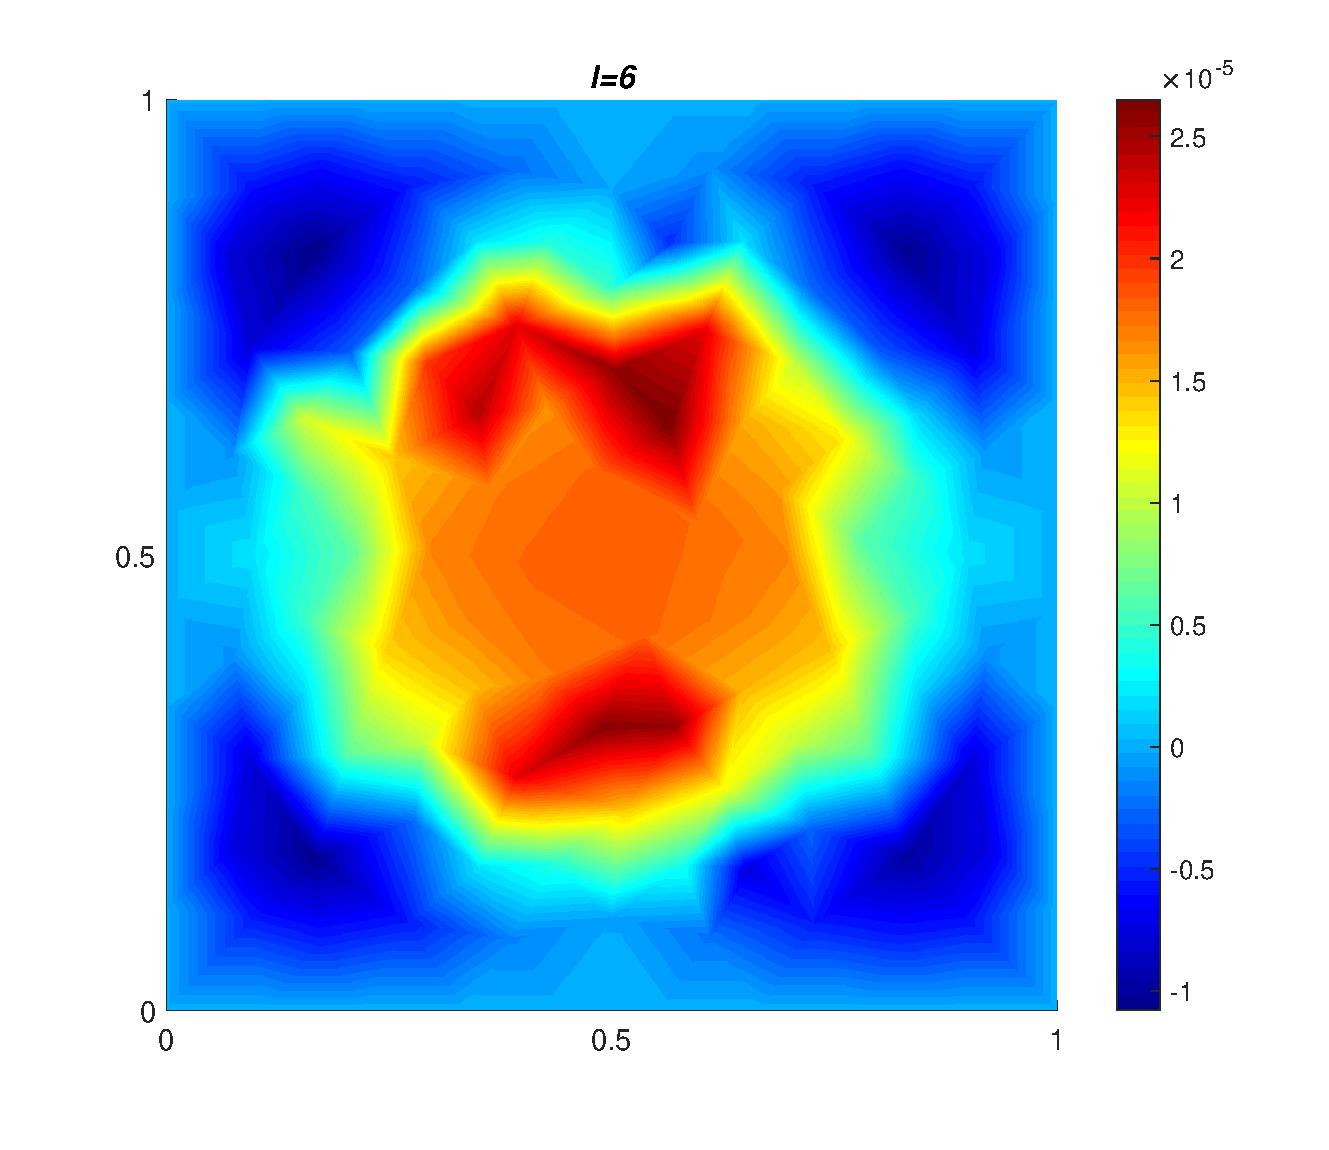
\includegraphics[width=0.42\textwidth,height=0.24\textheight]{plots/errorSurf_L4l6.eps}
 \caption{Comparison of error surface plots between intrusive and non-intrusive SSFEM for $L=4$ in the standard deviation of the solution process using $p_u=3,4,5$ and $l=3,4,5$ with respect to standard deviation of the solution process using $p_u=6$ and $l=6$}
 \label{fig:SD_errorSurf}
\end{figure}
%-----------------------------

%As a result, the computational cost of non-intrusive approach increases compared to intrusive approach.

%Form the plots given in \Cref{fig:5RV}, it became evident that the error gap between intrusive and non-intrusive solution coefficients increases with increase in the number of random variables.
In summary, from an implementational perspective the non-intrusive approach is favorable because one can directly employ any existing deterministic solver as a black box to simulate the required samples. On the other hand, the intrusive approach demands %reforming adjustments in the governing equations which necessitate
additional coding efforts. However, as demonstrated by the authors in~\cite{desai2017scalable,desai2019scalable}, the stochastic assembly procedure employed for intrusive SSFEM can utilize the readily available deterministic finite element assembly routines (such as FEniCS) which can substantially reduce the coding efforts.
Also, as demonstrated above, for a large number of random variables and a high order of PCE, the intrusive approach has better control over the error in the individual solution coefficients compared with the non-intrusive approach. Therefore, for practical applications which may require modeling of non-Gaussian (for example, lognormal process) system parameters requiring with large-number of random variables, the intrusive approach can be advantageous.

Despite the fact that the PCE based approaches (both intrusive and non-intrusive) can outperform the other approaches for many applications, they pose the following challenges:
\begin{itemize}
\item The PCE based approaches have difficulty in capturing sudden changes in the response (solution process), for example, predicting shock dynamics in the presence of uncertainties~\cite{lin2006predicting,wan2005adaptive,wan2006beyond} and responses of highly nonlinear aeroelastic systems which show an abrupt jump to a higher period limit cycle oscillations~\cite{liu2002non,lin2006predicting,desai2010analysis,desai2013uncertainty}.
\item The PCE solution has non-uniform convergence and tends to break down for long-time integration which is called the long-term degeneracy problem~\cite{lucor2004adaptive,wan2006long,desai2010analysis,desai2013uncertainty}.
\end{itemize}
To address these challenge various adaptive PCE methods are developed~\cite{li1998adaptive,le2004multi,lucor2004adaptive,wan2005adaptive,wan2006beyond}. %to alleviate the problem of long term degeneracy and discontinuity in the random space.
One such method is adaptive multi-element generalized PCE~\cite{wan2005adaptive,wan2006beyond}. The main idea of the this method is to adaptively decompose the space of random inputs into multiple elements and subsequently employ PCE at the element level. Similar technique but a nonintrusive multi-element PCE formulation is employed in~\cite{lucor2004adaptive} in order to predict the stochastic response in the presence of discontinuities in the random space.
In~\cite{le2004multi}, a multi-resolution analysis based on  multi-wavelet basis is applied to tackle uncertainty propagation in the complex and multidimensional stochastic problems. They conclude that the adaptive refinement of the multi-wavelet basis provides an attractive means to effectively tackle problems with steep or discontinuous dependence on random data.
The nonintrusive B-spline stochastic projection method is developed in order to capture the sharp discontinuities along with the long term periodic behavior in~\cite{millman2006uncertainty}. In another approach by Gerritsma et al.~\cite{gerritsma2010time}, as time progresses the new stochastic variables are defined and corresponding orthogonal polynomials are constructed to alleviate long-term degeneracy issue.
%With the new stochastic variables the solution can be represented exactly by lin- ear functions. This allows the method to use very low order polyno- mial approximations with high accuracies.
An algorithm based on constant phase interpolation was employed in~\cite{witteveen2009efficient,desai2013uncertainty} to deal with the long time degeneracy problems.
%Le Maitre et al. [31] used a similar principle in their work on the PCE with asynchronous time integration.}

% \newpage
Although we can readily accommodate the increased number of samples due to a large number of random variables in the non-intrusive approach, there is a substantial increase in the number of sample evaluations for the non-Gaussian input making it computationally costly compared to the intrusive approach. %for the same level of accuracy.
However, the memory required to assemble and solve the intrusive system increases as we increase the number of random variables. Therefore, for a computer with a fixed random access memory (RAM), there is an upper limit to the size of intrusive system we can accommodate. Nonetheless, if we can handle the increasing intrusive system size by distributing it among multiple nodes and employ an efficient parallel solver, we can get the solution coefficients quickly compared to the non-intrusive approach for the same level of accuracy.
%The non-intrusive approaches are embarrassingly parallel however, for large scale simulations, if the we cannot fit one sample in the memory of one core then we loose the embarrassingly parallel behavior of nonintrusive approach. On the other hand, in the intrusive approach, if the size of spacial resolution increases we can divide the problem in more subdomains.
For these reasons, in this research, we have focused on:
(a) the development of scalable domain decomposition solvers for intrusive SSFEM for two and three-dimensional stochastic PDEs and
(b) an efficient parallel implementation of these solvers utilizing high-performance computing (HPC) to solve the problems with high resolution in both spatial and stochastic domains.
Developing scalable solvers to tackle stochastic PDEs using SSFEM is an active area of research as evidenced by many articles published in the last couple of decades ~\cite{pellissetti2000iterative,le2003multigrid,chung2005efficient,elman2007solving,powell2009block,ghosh2009feti,ullmann2010kronecker,sousedik2014hierarchical,subber2014schwarz,subber2012PhDTh,powell2017efficient,stavroulakis2017gpu,pranesh2018feti}.
%Therefore, before we move on to the scalable DD-solvers and the efficient HPC implementation strategies devised in the current work, we review the existing literature about the available solution methods for the intrusive SSFEM in the following section.


%because we need to solve a much smaller set of equations.
%Domain decomposition methods can provide the necessary platform to divide the increased size of the intrusive system into smaller subsystems and then engage multiple computing cores to simulate these subsystems simultaneously~\cite{subber2012PhDTh,subberJCP2014,yagawa1991large}.
%The Krylov subspace based iterative solvers can be employed to solve the resulting system~\cite{subber2012PhDTh,subberJCP2014}.
%In the past, a variety of solution methods are proposed to solve the system of equations arising in the context of intrusive SSFEM. The brief overview of the available solution methods for SGFEM is given below.


%It is evident from the above results and discussion, the intrusive approach is a strong candidate to solve the stochastic system with a large number of random variables. The primary objective of this work is to solve the high-dimensional stochastic system, therefore, from here onwards we only focus on intrusive approach and its solution methods. There are various adaptive methods are proposed to improve the performance of non-intrusive SSFEM approaches~\cite{}. However, authors argue that the similar adaptivity can also be adapted for intrusive SSFEM. Therefore, those techniques are not focused in the current work. %, rather primary attention is given to develop efficient solution method for the SGFEM systems.


%%%%% Copied from JSV article %%%%%%


%%In this work, our main focus onto employing intrusive (Galerkin) approach. Hence we'll direct our attention onto it.
%%the resulting set of deterministic equation arising in the process of employing intrusive approach.
%For illustration purpose, let's consider $N$ spatial nodes, the finite element discretization  leads to the sparse system of equations of size $(N , N)$ as defined in Eq.~\ref{eq:Auf}.
%\begin{figure}[tbh]
%\centering
%\includegraphics[width=0.8\textwidth,height=0.34\textheight]{figures/ch2_SFEM/NpVp_forDiffL}
%\caption{For the fixed mesh resolution with a different $p$ and $L$.}
%\label{fig:NpVp}
%\end{figure}
%Incorporating PC expansions with $N_{p}$ terms and taking Galerkin projection leads to new block-sparse system of equation of size $(N \times N_p \ , N \times N_p)$ given by Eq.~\ref{eq:StoAuf}~[ref WaadTh-3, 37, 50]. The new problem we're solving is $N_p$ times bigger than original problem.
%The number of PCE terms required to represent the solution process $N_{p}$ is function of the order of basis functions ($p$) and the dimension of random variable ($L$). As both $p$ and $L$ increase, the number $N_{p}$ drastically increases as depicted in Figure~\ref{fig:NpVp}.
%With increasing $p$ if we use high dimensions ($L$), the number of PCE terms required to represent the solution process increases quickly. For example, in the case of $p=3$ with $L=3$ we need $N_{P} = 20$ and for same $p$ with $L=9$ we need $N_{p} = 220$ (both points are highlighted in Figure~\ref{fig:NpVp}).

%For practical engineering applications, where we need high resolution in both physical and stochastic dimension both $N$ and $N_{p}$ is large. In such cases the linear system of equations arising in the context of SSFEM becomes computationally challenging.
%Traditional solvers developed to tackle the system of equations obtained from deterministic FEM might not be useful for stochastic FEM.
%Therefore, we need parallel scalable solvers that can efficiently utilize the high-performance computing to handle such a large-scale systems.
%In the next section, we will focus onto the solution methods for the system formed using SSFEM.


% \section{Overview of Solution Methods for Intrusive SSFEM}\label{cp1:sec_mtdSSFEM}
% The system matrix obtained in the setting of intrusive SSFEM has a block sparsity structure as shown in \Cref{fig:SFEM1}. Each block of the system matrix has similar sparsity pattern to that of a deterministic finite element matrix. Therefore, the sparse direct solvers can be employed to solve the resulting system of equations~\cite{ghanem1996numerical,duff1986direct}.
% However, in the cases of intrusive SSFEM for large-scale system focused in this thesis, the sparse direct solvers demand more memory compared to iterative solvers.
% Thus, in the past, more attention has been given to the development of the sparse iterative solvers with the suitable preconditioners ($M^{-1}$)~\cite{ghanem1996numerical,pellissetti2000iterative,coupez1997directViteravie,saad2003iterative}.
% %Also, for the simulations with high resolution discretization in both spatial and stochastic domains which is the primary concern in this work, the direct solver is not a reasonable option.
% The preconditioned intrusive SSFEM system can be written as,
% \begin{equation} \label{preconBJ}
% M^{-1} [\mathcal{A}] \ \{\mathcal{U}\} = M^{-1} \ \{\mathcal{F}\}.
% \end{equation}
%
% Ghanem and Kruger (1996)~\cite{ghanem1996numerical} exercised preconditioned conjugate gradient method (PCGM) with block-Jacobi (BJ) preconditioner to solve the intrusive system of equations. The blocks of the preconditioner are obtained by LU factorization of the mean stiffness matrix.
% Another solution procedure based on hierarchical basis concepts was also proposed. In the second method, the intrusive SSFEM system is solved using the PCGM with an incomplete Cholesky factorization preconditioner.
% The performance of the PCGM equipped the BJ preconditioner is improved compared to the traditional Jacobi preconditioner. However, the number of PCGM iterations required for the convergence grows as the number of PCE terms increases.
%
%
% Pellissetti and Ghanem (1996)~\cite{pellissetti2000iterative} iteratively solved the intrusive system of equations arising using PCGM with a BJ preconditioner.
% They used the approximate inverse of each block of the matrix instead of LU decomposition.
% Taking the approximate inverse helps to preserve a prescribed sparsity structure, however, as the size of the matrix grows finding a good approximate inverse for the mean stiffness matrix is computationally expensive.
% Also, this preconditioner worked well for small random fluctuations, however for a high degree of uncertainty which requires a large number of PCE terms, the convergence rate of the BJ preconditioner deteriorates.
% %Hence, the only mean based preconditioners are not sufficient to solve the SGFEM of large-scale practical application.
%
% %Nair and Keane~\cite{nair2002stochastic} used stochastic reduced basis methods for solving large-scale linear random algebraic systems of equations, obtained by discretizing linear stochastic partial differential equation.
% %The system response is obtained by using a linear combination of stochastic basis vectors with undetermined deterministic coefficients. The preconditioned stochastic Krylov subspace is used to approximate the response process.
%
%
% Le Ma{\^i}tre et al. (2003) \cite{le2003multigrid}
% used a multigrid (MG) method based on spatial coarsening to solve the linear system arising in the setting of SSFEM for a two-dimensional stochastic diffusion equation.
% The computational tests conducted to analyze the behavior of the solver suggest that the MG scheme exhibits a fast rate of convergence and good scalability concerning spatial resolution.
% However, the convergence rate drops as the order of the PCE increases and it is heavily dependent on the level of the coefficient of variation (CoV) of the random system parameters.
% The convergence rate is slightly dependent on the correlation length of the stochastic diffusivity field, but it is very sensitive to MG parameters and cycle structure. Therefore, careful selection of these parameters is recommended.
%
% Chung et al.~\cite{chung2005efficient} employed an incomplete block-Jacobi preconditioner with block Gauss-Jacobi iterative method to solve the linear system in SSFEM.  An element-by-element strategy is employed for the matrix-vector product required for the iterative solver. This strategy is less expensive concerning memory as it requires the storage of the element stochastic stiffness matrix. However, after each matrix-vector multiplication step, the resulting vector needs to be assembled which consumes a large computation time.
% They concluded that the performance of the solver is not considerably affected by increasing the order of PCE. However, increase in CoV of the random input parameters drives the iteration counts.
%
%
% %Keese and Matthies (2005)~\cite{keese2005hierarchical} employed a hierarchical parallelization based solver for the solution of stochastic finite element system on a distributed memory architecture machine. A coarse-grained parallelization is implemented by constructing each block of the stochastic stiffness matrix and a fine level parallelization is implemented within each block.
% %These coarser levels are implemented by running different instances of the deterministic solver in parallel. The fine level of parallelization exploits the available deterministic parallel libraries to compute the matrix-vector multiplication and the preconditioner effect.
% %In this hierarchical parallelization approach, the time required to compute the preconditioner effect is inversely proportional to the number of processors.
%
%
% Elman and Furnival (2007)~\cite{elman2007solving} solved the stochastic steady-state diffusion problem formulated using the multigrid method.
% The spatial discretization is varied from grid to grid while the stochastic discretization is held constant.
% The mesh parameter is varied from the coarse grid to fine grid.
% Performing theoretical and experimental analysis, they concluded that the convergence rate of the solver is independent of the mesh resolution similar to the deterministic cases.
% However, the performance of the solver for varying stochastic parameters such a CoV and the number of PCE terms was not performed.
%
%
% Chao et al. (2007)~\cite{jin2007parallel} employed black-box additive Schwarz domain decomposition preconditioner with a recycling Krylov subspace method to solve the linear system of equation in intrusive SSFEM.
% Double orthogonal basis are used to decouple the probabilistic space resulting from a sequence of uncoupled systems of linear equations.
% They conclude that the preconditioner achieves a scalable performance concerning the number of subdomains and finite element mesh size. The recycling technique employed assists in reducing the total execution time.
%
%
% Rosseel et al. (2008)~\cite{rosseel2010iterative} used the algebraic multigrid method to tackle the linear system arising in the context of SSFEM. The hierarchy of meshes required for the multigrid method is built by using the mean stiffness matrix.
% The number of multigrid iterations is shown to be independent of the geometric mesh size for Gaussian and non-Gaussian material properties.
% In the case of uniform probability density function (pdf), the convergence rate of the proposed multigrid solver is proven to be asymptotically independent of the order of PCE. However, for a Gaussian pdf, it does not show similar behavior.
%
% %For the general material properties (Gaussian and non-Gaussian), the number of multigrid iterations is shown to be independent of the geometric mesh size.
%
%
% Powell and Elman (2009)~\cite{powell2009block} utilized block-diagonal preconditioner on the algebraic multigrid method to achieve optimal computational complexity. They provided a theoretical basis for the block-Jacobi preconditioner and established a bound for the condition number and highlight that these condition number bounds depend on the order of PCE, the number of random variables and coefficient of variation of the random system parameters. However, the performance of the algebraic multigrid scheme is shown to be independent of the size of the spatial discretization.
%
%
% Ghosh et al. (2009)~\cite{ghosh2009feti} exercised the incomplete block-diagonal preconditioner and its FETI-DP solver tailored for systems with multiple and repeated right-hand sides.
% A nested PCGM solver where outer PCGM for the full stochastic linear system an inner PCGM for the individual block of the preconditioner is used. To speed-up the convergence rate of the inner PCGM, a recycling Krylov subspace method is utilized.
% Performance tests of the solver demonstrated good numerical scalability concerning the number of subdomains and the size of the problem.
%
%
% Ullmann (2010)~\cite{ullmann2010kronecker} proposed a Kronecker product preconditioner obtained by exploiting the block sparsity structure of the stochastic stiffness matrix.
% The proposed preconditioner for the linear system arising in the context of SSFEM showed improved performance compared to the mean-based preconditioner.
% A moderate increase in the iteration counts is observed when the level of uncertainty in the system parameters and the order of the stochastic expansion increases.
% Furthermore, the Kronecker product preconditioner cannot be parallelized entirely due to the presence of the off-diagonal block elements.
%
%
% Soused{\'\i}k et al. (2014)~\cite{sousedik2014hierarchical} devised hierarchical Schur complement preconditioner for the intrusive SSFEM. This preconditioner is formed by exploiting the recursive hierarchy in the structure of the global matrices.
% One of the submatrices in the two-by-two recursive hierarchical structure is block diagonal and one of the diagonal blocks in this submatrix is similar to the deterministic mean-value problem.
% The numerical experiments performed on an elliptic problem demonstrate the superiority of hierarchical Schur complement preconditioner concerning iterations and work count over the block version of the symmetric Gauss-Seidel method.
%
%
% Subber and Loisel (2014)~\cite{subber2014schwarz} exercised a two-level additive Schwarz preconditioner for the iterative solution of the intrusive SSFEM system. It is based on partitioning the spatial domain while preserving all stochastic couplings. This preconditioner can be viewed as a generalization of the mean based BJ preconditioner. % commonly used in the literature.
% Their numerical analysis and computer experiments demonstrate that the convergence rate of stochastic Schwarz preconditioner is independent of the mesh parameters, the strength of randomness, dimension and order of the stochastic expansion in the cases of two-dimensional stochastic PDEs. Furthermore, the numerical simulations are performed to investigate condition number growth in regard to various system parameters.
%
%
% From our research group at Carleton university, Sarkar et al. (2009)~\cite{sarkarIJNME2009} introduced the domain decomposition method for uncertainty quantification of stochastic PDEs. The theoretical framework presented is based on Schur complement based domain decomposition in the physical space and functional decomposition in the stochastic dimension. A direct substructuring technique is implemented to solve a steady state wave propagation problem in one-dimensional random media. A dense direct solver is used to tackle the stochastic Schur complement system.
% This approach gives the ability to exploit the deterministic domain decomposition algorithms in the context of stochastic PDEs.
%
%
% Next, Subber and Sarkar (2013)~\cite{subberCMAME2013} formulated a probabilistic version of the dual-primal domain decomposition method for the intrusive SSFEM to exploit high-performance computing platforms for uncertainty quantification. In particular, they formulate a probabilistic version of the dual-primal finite element tearing and interconnect (FETI-DP) technique to solve the large-scale intrusive system of equations. In the probabilistic setting, the operator of the dual interface system in the dual-primal approach contains a coarse problem. The introduction of the coarse problem in the probabilistic setting leads to a scalable performance of the dual-primal iterative substructuring method for the cases of two-dimensional stochastic PDEs.
%
%
% Furthermore, Subber and Sarkar (2014)~\cite{subberJCP2014} introduced a two-level Neumann-Neumann preconditioner with vertex-based coarse grid to iteratively solve the large-scale intrusive SSFEM system. The implementation of the algorithm involves solving a local problem on each subdomain that constructs the local part of the preconditioner and a coarse problem that propagates information globally among the subdomains.
% The two-level preconditioner with the vertex-based coarse grid is shown to scale well for the cases with high mesh resolution and few random variables. However, for three-dimensional coupled stochastic PDE system, for instance, arising in the linear elasticity, the two-level Neumann-Neumann preconditioner and FETI-DP solvers with the vertex-based coarse grid showed a poor numerical and parallel scalabilities~\cite{subber2012PhDTh}.
%
%
% Drawing from the decade of experience of the group, in the recently published article by the author~\cite{desai2017scalable}, the intrusive polynomial chaos expansion based two-level domain decomposition algorithms are extended to concurrently handle high resolution in both spatial and stochastic domains. Sparse iterative solvers with efficient preconditioners are employed to solve the resulting global and subdomain level local systems through three-level nested iterative solvers. An efficient stochastic assembly procedure is employed to directly assemble and store blocks of stochastic finite element matrix using deterministic assembly matrix blocks. Sparse data structures, routines and solvers from PETSc are employed to handle subdomain level algebraic matrix-vector product and system solves. The NNC/BDDC and FETIDP solver are showed to handle large-scale simulations with a large number of random variables.
%
%
% Next, we have listed few of the recently published articles closely related the current work.
% Silvester and Pranjal (2016) in \cite{silvester2016optimal}  designed and implemented efficient solution algorithms for a symmetric positive-definite linear system arising in the context of stochastic Galerkin approximation of stochastic elliptic PDEs. They employed preconditioned MINRES solver with the incorporation of error control in the natural energy norm leading to a robust and optimally efficient stopping criterion. In their implementation, the iteration is terminated right after the algebraic error becomes insignificant compared to the approximation error.
%
%
% Powell et al. (2017)~\cite{powell2017efficient} reformulated the system of equations arising in the setting of stochastic Galerkin finite element approximation of stochastic PDEs as multiterm linear matrix equations. They generalized the ideas from rational Krylov subspace approximation to develop an efficient solution algorithm.
% A low-rank approximation to the solution matrix is determined by performing a projection onto a low-dimensional space to get an efficient solution strategy with the convergence rate independent of the spatial discretization. They conclude that the new strategy takes considerably less memory than the standard mean-based PCGM applied to the Kronecker formulation of the linear systems.
% %They assume that the number of random variables characterizing the random inputs is modest and that the dependence on these variables is linear, so that it is sufficient to seek only a reduction in the complexity associated with the spatial component of the approximation space.
%
%
% Stavroulakis et al. (2017)~\cite{stavroulakis2017gpu} employed graphics processing units (GPU) based domain decomposition solution for spectral stochastic finite element method. They demonstrate the benefits of employing the GPU capabilities in addressing intrusive SSFEM by using the dual domain decomposition method preconditioners tailored for the specific applications. Their results showed a significant enhancement in the computational performance as well as of the consumed energy efficiency in the spectral stochastic finite element method.
%
%
% Pranesh and Ghosh (2018)~\cite{pranesh2018feti}
% devised a parallel domain decomposition-based hybrid method combining Monte Carlo simulation with stochastic Galerkin approach for solving large-scale problems.
% In their approach, the dual-primal variant of the FETI-DP is chosen as the domain decomposition method followed by three distinct strategies of parallel implementation.
% Performing numerical experiments the best approach is selected to solve a three-dimensional elasticity problem with high-dimensional parametric uncertainty and low order of expansion.
% %The computational cost of uncertainty propagation in a mechanics problem can become prohibitively large as the degrees of freedom (DOF) and the number of basic random variables � also referred to as stochastic dimensionality � increase. While a number of methods have been reported in the literature to address either large DOF or high stochastic dimensionality, there is no work addressing both. This work is aimed at filling this gap. Naturally, parallel computing becomes the only feasible option for these large problems. Accordingly,

%-------------APPENDIX----------------
\section{Non-Intrusive SSFEM}\label{apn:nisp}
% In the NISP approach, the Galerkin projection is directly performed on to the PCE of the solution process given in \Cref{eq:pce}. The orthogonality properties of PCE basis polynomials are utilized to compute the expansion coefficients of the solution process~\cite{ghanemSFEM1991,le2010spectral,le2010spectral}.
Performing Galerkin projection onto the PC expansion of solution process given in \Cref{eq:pce} and then exploiting orthogonality properties of the basis functions, the PCE coefficients of the solution process can be evaluated as follows~\cite{ghanemSFEM1991,le2010spectral,xiu2009fast};
\begin{equation}
{\mathrm{\hat{\bf{u}}}_k}   = \frac{\left< {\mathrm{\bf{u}(\theta)}} {\Psi_k({\pmb{\xi}})}  \right>} {\left< {\Psi_j({\pmb{\xi}})} {\Psi_k({\pmb{\xi}})}  \right>} = \frac{1} {\left<{\Psi_k({\pmb{\xi}})^{2}}  \right>} \int_{\Omega} {\mathrm{\bf{u}(\theta)}} {\Psi_k({\pmb{\xi}})} {\mathrm{p}}(\pmb{\xi}) {d{\pmb{\xi}}},
\label{eq:apn_NISPpce}
\end{equation}
where $\left< {\Psi_j({\pmb{\xi}})} {\Psi_k({\pmb{\xi}})}  \right>$ is non-zero only for $j=k$ and it can be obtained analytically beforehand~\cite{smith2013uncertainty,desai2019scalable}.
%, for instance see \Cref{table:hpoly}.
Therefore, the major computational efforts lies in the evaluation of the multidimensional integral in the numerator of \Cref{eq:apn_NISPpce}~\cite{le2010spectral,reagana2003uncertainty,hosder2006non,ganapathysubramanian2007sparse,nobile2008sparse}.
%In the past, random sampling, tensor product quadrature or sparse grid quadrature based approaches were employed to solve the integral
%in the numerator of \Cref{eq:apn_NISPpce} ~\cite{le2010spectral,reagana2003uncertainty,hosder2006non,ganapathysubramanian2007sparse,nobile2008sparse}.

The efficient evaluation of the multidimensional integral in \Cref{eq:apn_NISPpce} is key part in the implementation of of this NISP approach especially for the high dimensional stochastic cases.
Consider the FE discretization of a stochastic PDE given in \Cref{eq:dFEM}. Using $\{ \pmb{\xi}_{1} ,  \pmb{\xi}_{2} , \dots, \pmb{\xi}_{n_{s}}  \}$ (where $\pmb{\xi}_i$ is a set of $L$ random variables), the following deterministic system is solved at $n_{s}$ sample points using an existing deterministic solver as a black-box.
\begin{equation}\label{eq:apn_nispSamp}
{\mathrm{\bf{A}(\theta)  \bf{u}(\theta) = \bf{f}}}.
\end{equation}
Computed $\bf{u}(\theta)$ at each sample points are used to calculate the PCE coefficients of the solution process using Smolyak sparse grid quadrature~\cite{le2010spectral,hosder2006non,ganapathysubramanian2007sparse,nobile2008sparse,eldred2009recent,debusschere2013uqtk}.
%The various advanced sampling strategies were reported in past few years~[refer \cite{} articles and references therein].

The sparse grid nodal set for $d=2$ and $l=3$ can be written as~\cite{smith2013uncertainty}
\begin{align}\label{eq:sparseNodes}
  \Theta_{l=3}^{(d=2)} &= \bigcup_{|l'| \leq l+d-1} \Big( \Theta_{l_1}^{(1)}  \times \Theta_{l_2}^{(1)}  \Big) \\ \nonumber
  &= \Big( \Theta_{1}^{(1)}  \times \Theta_{1}^{(1)}  \Big)  \ \ \ \ \ (l_1=1, l_2=1) \\ \nonumber
  &\cup \Big( \Theta_{1}^{(1)}  \times \Theta_{2}^{(1)}  \Big) \cup \Big( \Theta_{2}^{(1)}  \times \Theta_{1}^{(1)}  \Big)
  \\ \nonumber
  &\cup \Big( \Theta_{1}^{(1)}  \times \Theta_{3}^{(1)}  \Big)  \cup \Big( \Theta_{2}^{(1)}  \times \Theta_{2}^{(1)}  \Big)  \cup \Big( \Theta_{3}^{(1)}  \times \Theta_{1}^{(1)}  \Big),
\end{align}
where $l'=(l_1 \dots l_d)$ with $|l'| = \sum_{i=1}^d l_i$
% The nodal set $\Theta$ for the sparse grid can be obtained using one-dimensional sparse nodal set $\Theta_{l}^{(1)}$ as~\cite{smith2013uncertainty}.
(a specific example to obtain the sparse grid nodal set involving  $\Theta_{1}^{(1)} \times \Theta_{2}^{(1)}$ is given below).
% The recursive formula for the $d$-dimensional Smolyak integral ${\mathscr{Q}}_{l}^{(d)}$ of the multidimensional function ${\mathscr{F}}$ can be written as~\cite{garcke2014sparse}
% \begin{equation}\label{eq:apn_sgND}
% {\mathscr{Q}}_{l}^{(d)} \ {\mathscr{F}} = \Bigg( \sum_{i=1}^{l} \Big( {\mathscr{Q}}_{i}^{(1)} - {\mathscr{Q}}_{i-1}^{(1)}  \Big)  \otimes {\mathscr{Q}}_{l-i+1}^{(d-1)}  \Bigg) {\mathscr{F}},
% \end{equation}
% where $l$ is the level of sparse grid.
% Equivalent formulation of the Smolyak sparse grid can be found in following articles with slightly different notations~\cite{eldred2009recent,smith2013uncertainty,le2010spectral}.
%
% \newpage
% The recursive formula given in \Cref{eq:apn_sgND} can be expanded, for instance, using $l=1, 2$ and $3$ with $d=2$ to get,
% \begin{align}\label{eq:sgNDeg1}
% {\mathscr{Q}}_{3}^{(2)} \ {\mathscr{F}} &= {\mathscr{Q}}_{1}^{(d=2)} + {\mathscr{Q}}_{l=2}^{(d=2)} + {\mathscr{Q}}_{l=3}^{(d=2)}
% \\ \nonumber &= \Bigg( \sum_{i=1}^{l=1} \Big( {\mathscr{Q}}_{i}^{(1)} - {\mathscr{Q}}_{i-1}^{(1)}  \Big)  \otimes {\mathscr{Q}}_{1-i+1}^{(2-1)}  \Bigg) {\mathscr{F}}
% + \Bigg( \sum_{i=1}^{2} \Big( {\mathscr{Q}}_{i}^{(1)} - {\mathscr{Q}}_{i-1}^{(1)}  \Big)  \otimes {\mathscr{Q}}_{2-i+1}^{(2-1)}  \Bigg) {\mathscr{F}} \\ \nonumber
% &+ \Bigg( \sum_{i=1}^{3} \Big( {\mathscr{Q}}_{i}^{(1)} - {\mathscr{Q}}_{i-1}^{(1)}  \Big)  \otimes {\mathscr{Q}}_{3-i+1}^{(2-1)}  \Bigg) {\mathscr{F}}
% \\ \nonumber &= \Bigg( \Big( {\mathscr{Q}}_{1}^{(1)} - {\mathscr{Q}}_{0}^{(1)}  \Big)  \otimes {\mathscr{Q}}_{1}^{(1)}  \Bigg) {\mathscr{F}} + \Bigg( \Bigg[ \Big( {\mathscr{Q}}_{1}^{(1)} - {\mathscr{Q}}_{0}^{(1)}  \Big)  \otimes {\mathscr{Q}}_{2}^{(1)}  \Bigg] + \Bigg[ \Big( {\mathscr{Q}}_{2}^{(1)} - {\mathscr{Q}}_{1}^{(1)}  \Big)  \otimes {\mathscr{Q}}_{1}^{(1)}  \Bigg]  \Bigg){\mathscr{F}} \\ \nonumber
% &+  \Bigg( \Bigg[ \Big( {\mathscr{Q}}_{1}^{(1)} - {\mathscr{Q}}_{0}^{(1)}  \Big)  \otimes {\mathscr{Q}}_{3}^{(1)}  \Bigg] + \Bigg[ \Big( {\mathscr{Q}}_{2}^{(1)} - {\mathscr{Q}}_{1}^{(1)}  \Big)  \otimes {\mathscr{Q}}_{2}^{(1)}  \Bigg] + \Bigg[ \Big( {\mathscr{Q}}_{3}^{(1)} - {\mathscr{Q}}_{2}^{(1)}  \Big)  \otimes {\mathscr{Q}}_{1}^{(1)}  \Bigg] \Bigg){\mathscr{F}}.
% \end{align}
% % \begin{align}\label{eq:sgNDeg2} \nonumber
% % {\mathscr{Q}}_{l=2}^{(d=2)} \ {\mathscr{F}} &= \Bigg( \sum_{i=1}^{l=2} \Big( {\mathscr{Q}}_{i}^{(1)} - {\mathscr{Q}}_{i-1}^{(1)}  \Big)  \otimes {\mathscr{Q}}_{2-i+1}^{(2-1)}  \Bigg) {\mathscr{F}}, \\ \nonumber
% % &= \Bigg( \Bigg[ \Big( {\mathscr{Q}}_{1}^{(1)} - {\mathscr{Q}}_{0}^{(1)}  \Big)  \otimes {\mathscr{Q}}_{2}^{(1)}  \Bigg] + \Bigg[ \Big( {\mathscr{Q}}_{2}^{(1)} - {\mathscr{Q}}_{1}^{(1)}  \Big)  \otimes {\mathscr{Q}}_{1}^{(1)}  \Bigg]  \Bigg){\mathscr{F}}, \\
% %  &= \Bigg( \Bigg[ {\mathscr{Q}}_{1}^{(1)}  \otimes {\mathscr{Q}}_{2}^{(1)}  \Bigg]
% %  + \Bigg[ {\mathscr{Q}}_{2}^{(1)}  \otimes {\mathscr{Q}}_{1}^{(1)}  \Bigg] \Bigg) {\mathscr{F}}.
% % \end{align}
% Therefore sparse grid quadrature for $l=2$ and $d=2$ can be obtained by using \Cref{eq:sgNDeg1} as
% \begin{align}\label{eq:sgNDeg}
% {\mathscr{Q}}_{2}^{(2)} \ {\mathscr{F}} &= \Bigg(
% \Bigg[ {\mathscr{Q}}_{1}^{(1)}  \otimes {\mathscr{Q}}_{1}^{(1)} \Bigg]
% + \Bigg[ {\mathscr{Q}}_{1}^{(1)}  \otimes {\mathscr{Q}}_{2}^{(1)}  \Bigg]
%  + \Bigg[ {\mathscr{Q}}_{2}^{(1)}  \otimes {\mathscr{Q}}_{1}^{(1)} \Bigg] \\ \nonumber
%  &+ \Bigg[ {\mathscr{Q}}_{1}^{(1)}  \otimes {\mathscr{Q}}_{3}^{(1)} \Bigg]
%  + \Bigg[ {\mathscr{Q}}_{2}^{(1)}  \otimes {\mathscr{Q}}_{2}^{(1)} \Bigg]
%  + \Bigg[ {\mathscr{Q}}_{3}^{(1)}  \otimes {\mathscr{Q}}_{1}^{(1)} \Bigg]
%  \Bigg) {\mathscr{F}}.
% \end{align}
% \begin{align}\label{eq:sgNDeg2} \nonumber
% {\mathscr{Q}}_{l=3}^{(d=2)} \ {\mathscr{F}} &= \Bigg( \sum_{i=1}^{l=3} \Big( {\mathscr{Q}}_{i}^{(1)} - {\mathscr{Q}}_{i-1}^{(1)}  \Big)  \otimes {\mathscr{Q}}_{l-i+1}^{(2-1)}  \Bigg) {\mathscr{F}}, \\ \nonumber
% {\mathscr{Q}}_{3}^{(2)} \ {\mathscr{F}} &= \Bigg( \Bigg[ \Big( {\mathscr{Q}}_{1}^{(1)} - {\mathscr{Q}}_{0}^{(1)}  \Big)  \otimes {\mathscr{Q}}_{3}^{(1)}  \Bigg] + \Bigg[ \Big( {\mathscr{Q}}_{3}^{(1)} - {\mathscr{Q}}_{1}^{(1)}   \Big)  \otimes {\mathscr{Q}}_{2}^{(1)}  \Bigg] + \Bigg[ \Big( {\mathscr{Q}}_{2}^{(1)} - {\mathscr{Q}}_{1}^{(1)}   \Big)  \otimes {\mathscr{Q}}_{1}^{(1)}  \Bigg]  \Bigg){\mathscr{F}}, \\
% {\mathscr{Q}}_{3}^{(2)} \ {\mathscr{F}} &= \Bigg( \Bigg[ {\mathscr{Q}}_{1}^{(1)}  \otimes {\mathscr{Q}}_{3}^{(1)}  \Bigg]
% + \Bigg[ {\mathscr{Q}}_{2}^{(1)}  \otimes {\mathscr{Q}}_{2}^{(1)}  \Bigg] + \Bigg[ {\mathscr{Q}}_{3}^{(1)}  \otimes {\mathscr{Q}}_{1}^{(1)}  \Bigg] \Bigg) {\mathscr{F}}.
% \end{align}
%For high dimensions $d$ and the higher level of quadrature $l$, the sparse tensor product formula can drastically reduce the number of quadrature points~\cite{ganapathysubramanian2007sparse,nobile2008sparse,eldred2009comparison}.
%Equivalently, the Smolyak formula can also be written directly using $ \mathscr{U}^{(1)}_{l}$ as
% \begin{equation}\label{sg2}
%\mathscr{A}_{l}^{n} \ {\bf{u}_{f}}= \sum_{{(l+n)\leq |\mathrm{\bf{i}}|\leq}(l+n-1)}  (-1)^{(l+n)-{|\mathrm{\bf{i}}|}} \binom{n-1}{(l+n) - {|\mathrm{\bf{i}}|}} . (\mathscr{U}^{i_{1}} \otimes \dots \otimes\mathscr{U}^{i_{n}} )
%\end{equation}
%The level of quadrature $l$ is independent of dimension.
%The Smolyak formula is sparse tensor product formula (i.e. a fewer points are used in each dimension as compared to full tensor product grid).
% \newpage
For the implementation of the multidimensional sparse grid the growth rule in one-dimensional quadrature must be defined. In the current implementation, we have used the Gauss-Hermite quadrature rule~\cite{eldred2009recent,smith2013uncertainty}.
%For further details on the types of growth rules available and their performance comparisons refer the following articles and reference therein~\cite{ganapathysubramanian2007sparse,nobile2008sparse,eldred2009recent,smith2013uncertainty}.
For further simplification, consider the Gauss-Hermite quadrature rule in one dimension with the nodes and weight specified in \Cref{table:sparseGrid}, for different level of quadrature.


\

\begin{table}[htbp]
\centering
\begin{tabular}{|l|c|c|}   %l-left c-center
\hline
level $l$    & nodes $\Theta_l^{(1)}$  & weights $\mathcal{W}_l^{(1)}$\\
\hline
$l=1$      & $\{0 \}$   & $\{ 1 \}$       \\
$l=2$      & $\{-1,  1\}$   & $\{0.5, 0.5\}$       \\
$l=3$      & $\{ -1.7321, 0, 1.7321 \}$ & $\{ 0.167, 0.667, 0.167 \}$       \\
\hline
\end{tabular}
\caption{Nodes and weights for Gauss-Hermite quadrature in one dimension and third level.}
\label{table:sparseGrid}
\end{table}

Using \Cref{eq:sparseNodes}, \Cref{eq:sg1D} and \Cref{eq:sparseDifference}, the nodes and weight for $l=3$ and $d=2$ are obtained as shown in \Cref{table:l2d2sparseGrid}.

\

\begin{table}[htbp]
\centering
\begin{tabular}{|l|c|}   %l-left c-center
\hline
nodes $\Theta_2^{(2)}$  & weights $\mathcal{W}_2^{(2)}$ \\
\hline
$\{ -1.732, 	0 \}$ & 0.167\\
$\{ -1.0, 	-1.0\}$ & 0.25 \\
$\{ -1.0, 	0 \}$& -0.5 \\
$\{ -1.0,  1.0\}$ & 0.25 \\
$\{ 0,	 -1.732 \}$& 0.167 \\
$\{ 0,	 -1.0\}$ & -0.5 \\
$\{ 0,	 0 \}$& 1.333 \\
$\{ 0, 1.0 \}$& -0.5 \\
$\{ 0,	 1.732\}$ & 0.167 \\
$\{1.0, 	-1.0 \}$& 0.25 \\
$\{1.0, 	0  \}$& -0.5 \\
$\{1.0, 	1.0\}$ & 0.25 \\
$\{1.732, 	0 \}$& 0.167\\
\hline
\end{tabular}
\caption{Nodes and weights for Gauss-Hermite quadrature in two dimension and third level.}
\label{table:l2d2sparseGrid}
\end{table}

\newpage
The relations in~\Cref{eq:sparseNodes} are used to get the set of nodes in \Cref{table:l2d2sparseGrid}. For instance, the nodes for $\big( \Theta_1^{(1)}  \times \Theta_2^{(1)} \big)$ are obtained by taking tensor produt of $\Theta_1^{(1)} = \{ 0 \}$ and $\Theta_2^{(1)} = \{ -1, 1 \}$, resulting into the following set of nodes = $\big[ \{0, -1\}, \{0, 1\} \big]$ which correspond to the $6^{rd}$ and the $8^{th}$ row in the first column of \Cref{table:l2d2sparseGrid}. The difference relation given in~\Cref{eq:sparseDifference} is used to get the corresponding weights~\cite{smith2013uncertainty} (refer to the example given in~\Cref{sec:NI} for more details about the weights of the sparse grid quadrature).

%--------------------CHAPTER 3------------------
\subsubsection{Scalability using Large-Scale HPC Cluster}
%large scale computing facilities
In a second set of experiments, we study the numerical scalability of the BDDC/NNC-PCGM solver for a highly dense mesh having $0.332$ million nodes and $0.664$ million elements.
%with a fixed number of PCE terms $P_u = 56$.
The number of cores utilized for these experiments vary from $1000$ to $4000$. The number of PCE terms ranges from 20 to 220 and the order of expansion $p_u=3$ is kept constant.
The scalability results with respect to the number of subdomains and the number of PCE terms are plotted in~\Cref{fig:cedar_nIterVnProc} and \Cref{fig:cedar_nIterVnPCE} respectively. These plots indicates that the solver is numerically scalable with large-scale computing clusters
%with up to $4000$ cores.
Similarly, the results in \Cref{fig:cedar_nIterVnProc} shows an excellent strong parallel scaling with thousands of cores.
\begin{figure}[htbp]
\centering
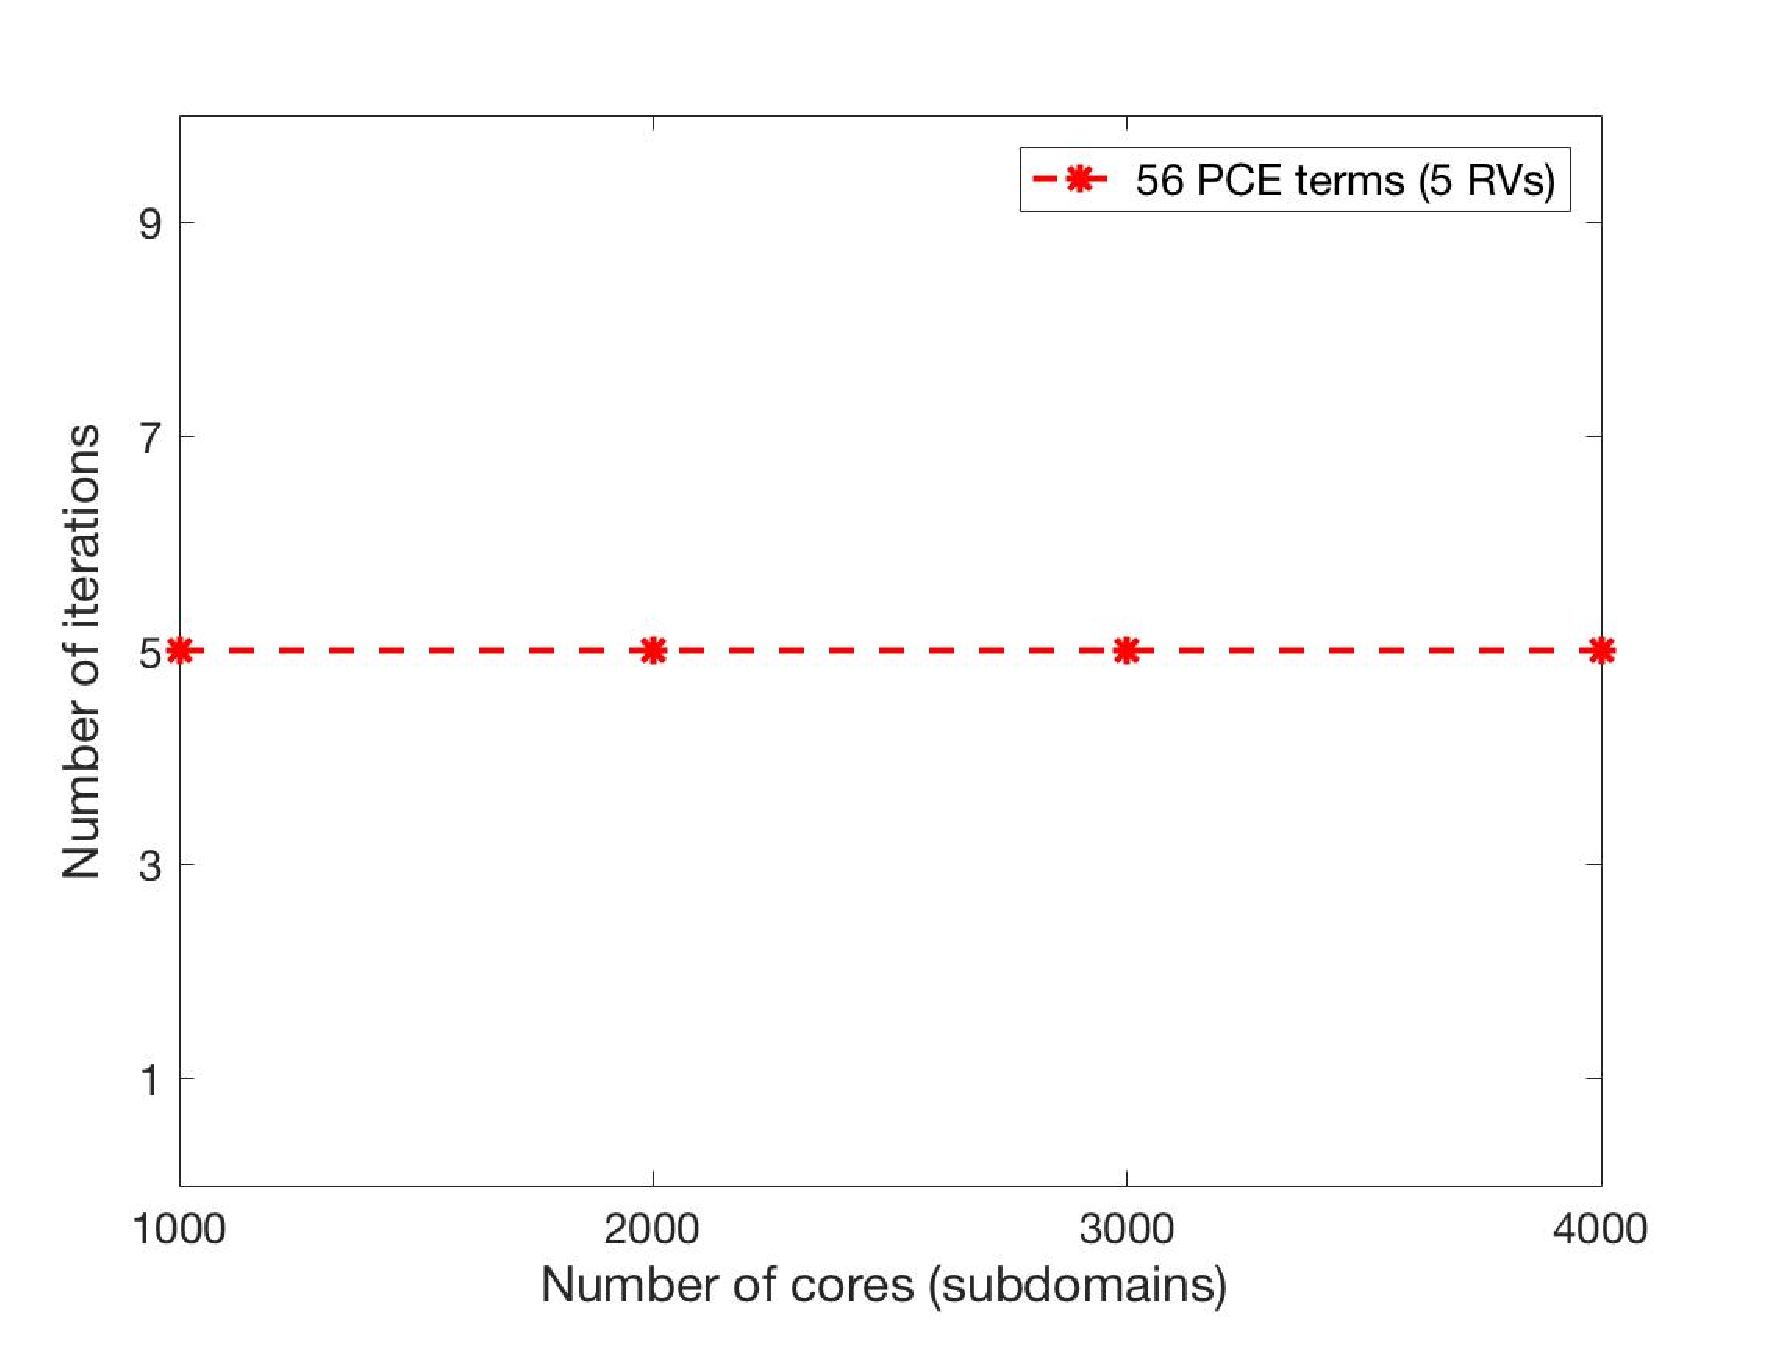
\includegraphics[width=0.65\textwidth,height=0.35\textheight]{plots/cedar_nIterVnProc.eps}
\caption{Iteration count versus number of subdomains for the fixed mesh resolution with fixed number of PCE terms.}
\label{fig:cedar_nIterVnProc}
\end{figure}
\begin{figure}[htbp]
\centering
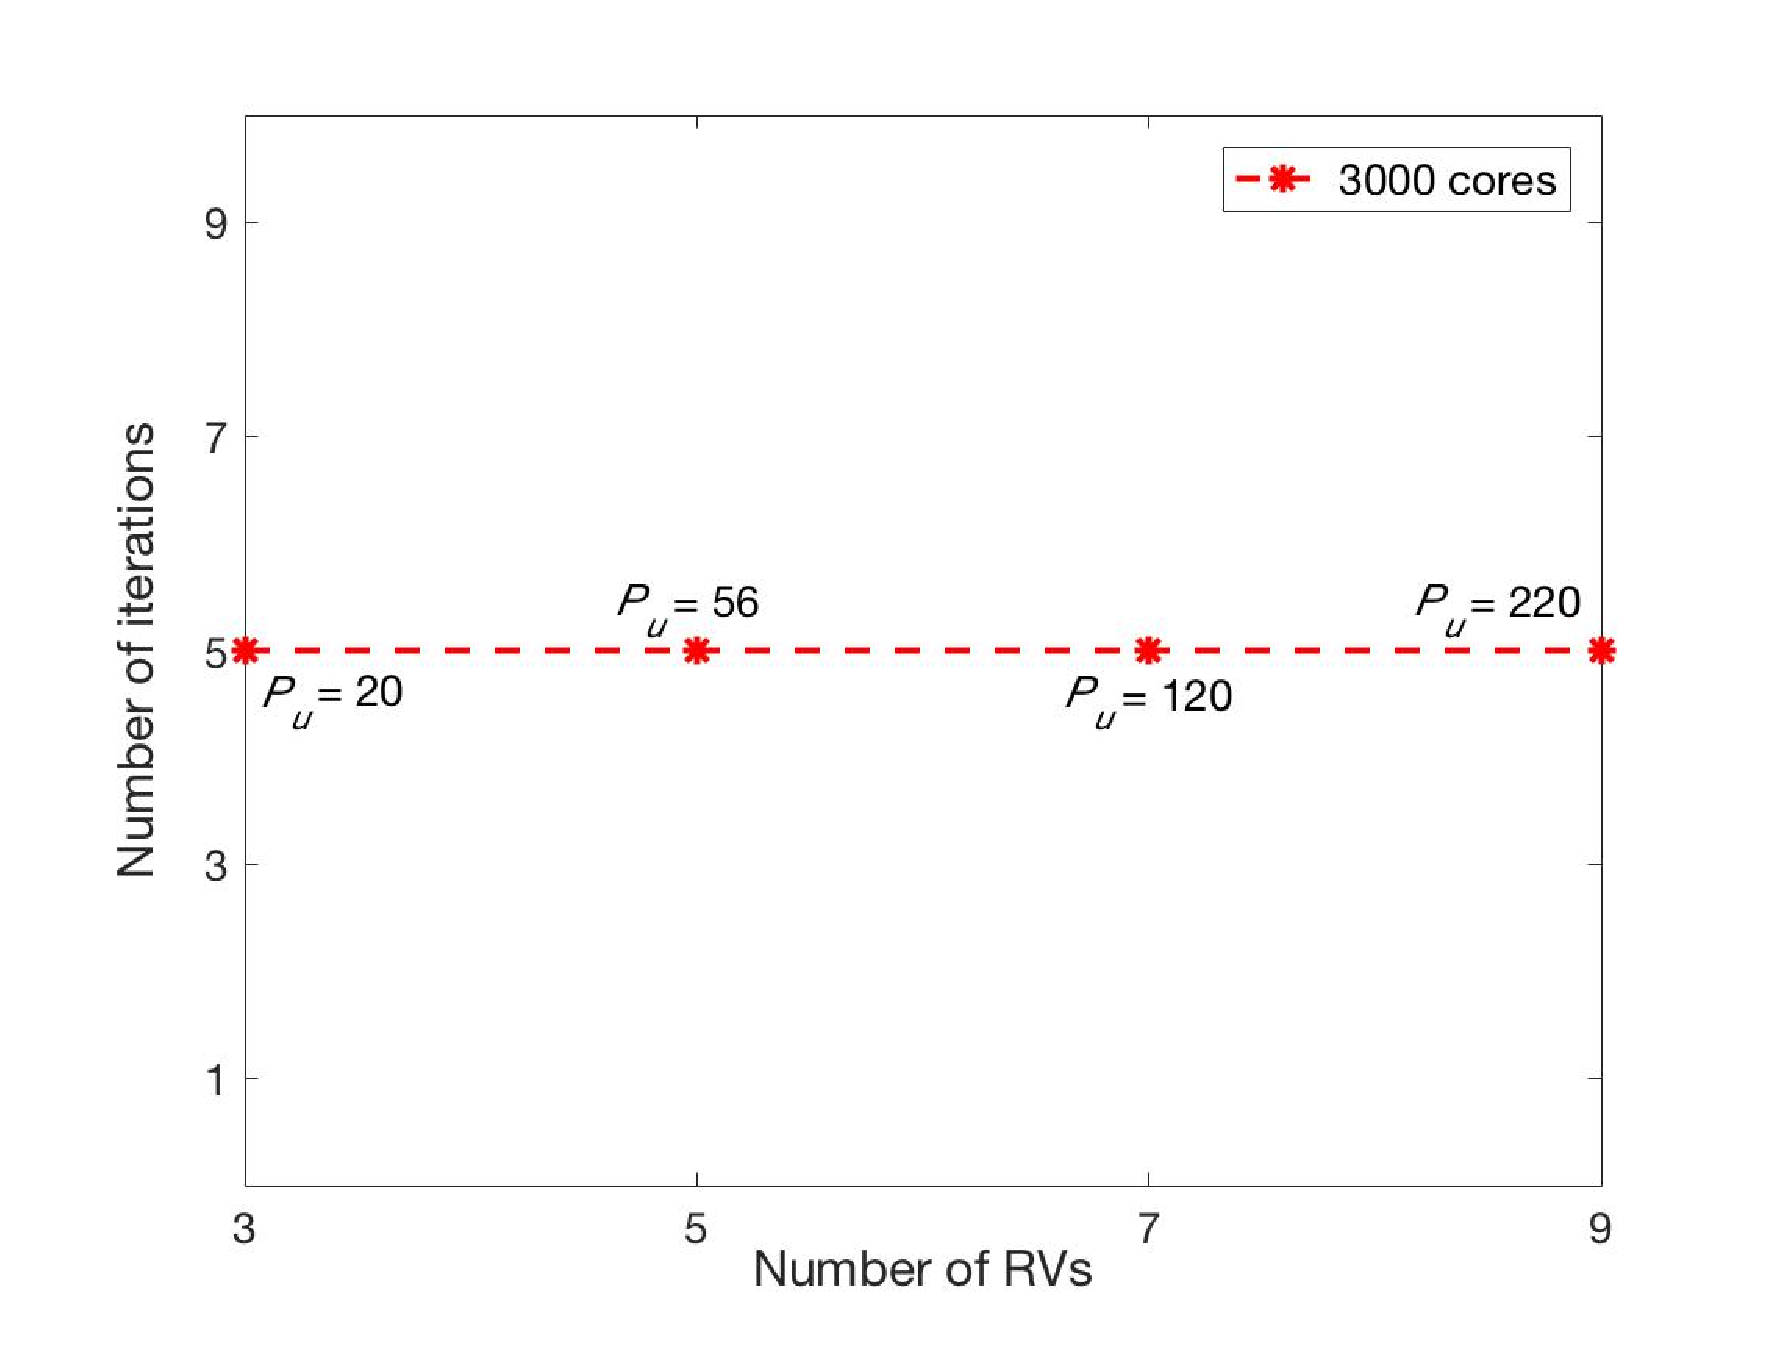
\includegraphics[width=0.68\textwidth,height=0.35\textheight]{plots/cedar_nIterVnPCE.eps}
\caption{Iteration count versus number PCE terms for the fixed mesh resolution with fixed number of subdomains.}
\label{fig:cedar_nIterVnPCE}
\end{figure}
\begin{figure}[htbp]
\centering
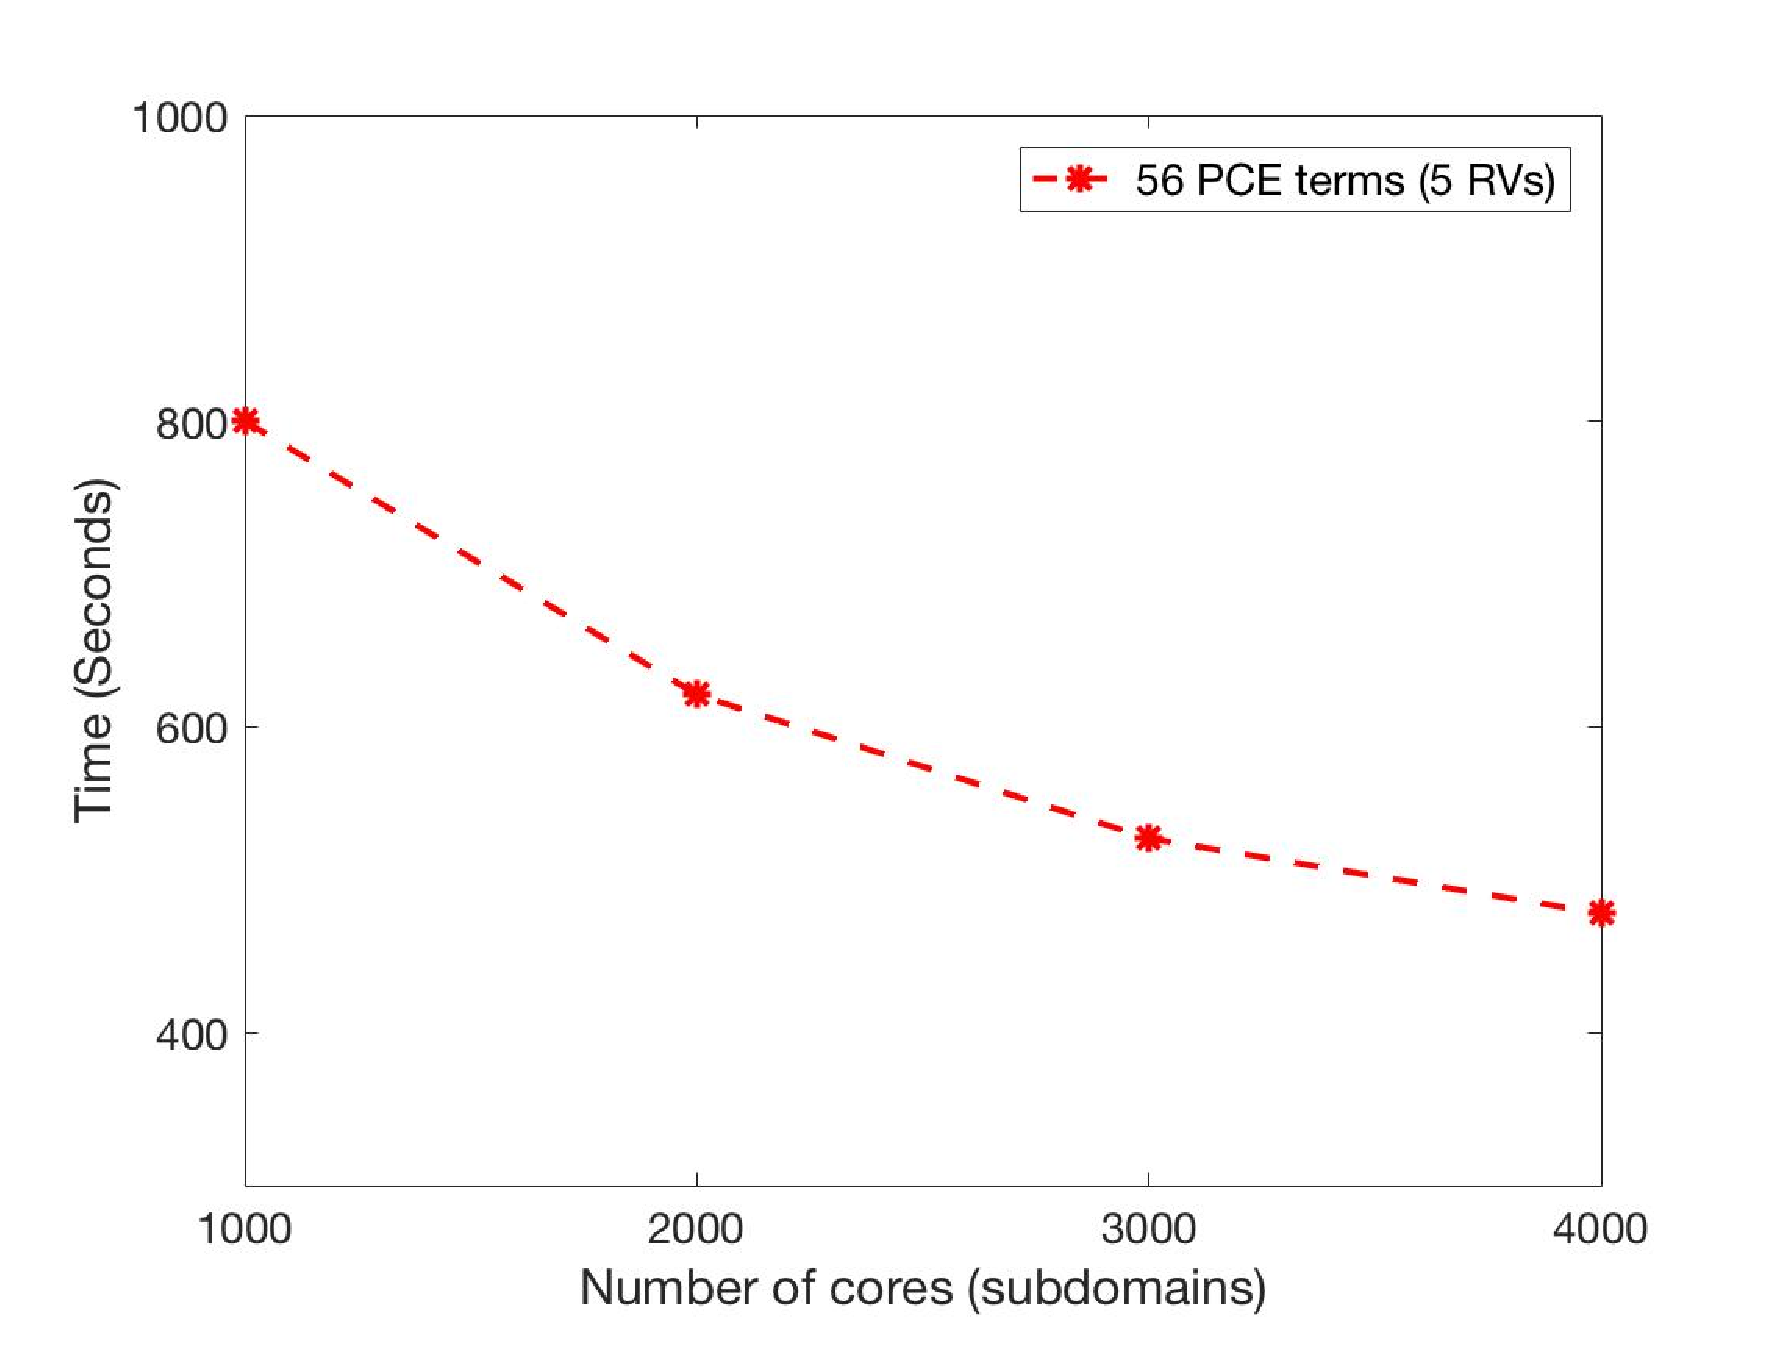
\includegraphics[width=0.65\textwidth,height=0.35\textheight]{plots/cedar_timeVsProcs.eps}
\caption{Execution time versus number of subdomains with the fixed mesh resolution and the fixed number of PCEs.}
\label{fig:cedar_timeVsProcs}
\end{figure}

\

Furthermore, using PETSc{\it{-log-view}}, the total floating-point operations of all cores, average and maximum/minimum floating-point operations among cores are estimated against various numbers of cores used to solve the SSFEM system in the second set of experiments.
The results are summarized in \Cref{table:tableCP31} and \ref{table:tableCP32} below.
%for a different number of PCE terms with the fixed number of cores and in \Cref{table:tableCP32} for a different number of cores with a fixed number of PCE terms.
\Cref{table:tableCP31} indicates, for a fixed problem size (both mesh resolution and the number of PCE terms are fixed), if we increase the number of cores, the total and average floating-point operations count decreases due to the decrease in workload per core as more cores are engaged.
\Cref{table:tableCP32} indicates, for a fixed number of cores ($n_s=4000$), both average and total floating-point operations count increases with the increasing number of PCE terms, emphasizing the increased workload per core.
The total floating-point operations required in the case of $P_u=364$ reached $1.728$ Petaflop. The results emphasize the necessity of using large-scale computing clusters and importance of scalable solvers for uncertainty propagation. Further increase in the number of RVs could demand a computing cluster capable of $10^{18}$ floating-point operations, pointing to emerging {\it{exascale}} computing~\cite{ashby2010opportunities,duff2011european}.
From the perspective of load balancing, the maximum to minimum floating-point operations ratio among the cores is far from 1 indicating workload imbalance. Further investigation is needed to fine-tune the parallel implementation to achieve efficient load balancing.

\

\begin{table}[htbp]
\centering
\begin{tabular}{l*{6}{c}r}
%\multicolumn{1}{ c }{} & \multicolumn{6}{ c }{$N_{s}$}
\hline
Fixed PCE ($P_u = 56$) & Total (Petaflop) & Average (Teraflop) & Max/Min \\
\hline
$N_s=1000$ & 0.1684 & 0.1684 & 1.87000 \\ \hline
$N_s=2000$ & 0.1255 & 0.0627 & 1.99444 \\ \hline
$N_s=3000$ & 0.1195 & 0.0395 & 1.78914 \\ \hline
$N_s=4000$ & 0.1201 & 0.0300 & 1.85542 \\
\hline
\end{tabular}
\caption{Floating-point operations for different number of cores with the fixed number of PCE terms}
\label{table:tableCP31}
\end{table}

\begin{table}[htbp]
\centering
\begin{tabular}{l*{6}{c}r}
%\multicolumn{1}{ c }{} & \multicolumn{6}{ c }{$N_{s}$}
\hline
Fixed cores ($N_s = 4000$) & Total (Petaflop) & Average (Teraflop) & Max/Min \\
\hline
%$P_u=20$ & 0.0262 & 0.0065  & 1.98056 \\ \hline
$P_u=56$  & 0.1232 & 0.0308  & 1.85542  \\ \hline
$P_u=120$ & 0.7884 & 0.1971 & 2.00349 \\ \hline
$P_u=220$ & 1.0448 & 0.2612 & 1.99514 \\ \hline
$P_u=364$ & 1.7281 & 0.4320 & 1.85249 \\
\hline
\end{tabular}
\caption{Floating-point operations for different number of PCE terms with the fixed number of cores}
\label{table:tableCP32}
\end{table}

\subsection{Comparison with Non-Intrusive SSFEM at High Dimensions}
To demonstrate the superiority of intrusive SSFEM equipped with scalable parallel DD solvers, consider a finite element mesh with $52704$ nodes and $105410$ triangular elements.
The intrusive SSFEM systems formulated by using the fixed $p_{u}=3$ and four different cases by selecting the number of RVs as $L=5, 10, 15$ and $20$ are considered. For the parallel solution, we employed BDDC/NNC solver using $80, 160, 240$ and $320$ cores respectively.
For the same cases, the sparse grid with the level of quadrature, $l=3$ and $l=4$ are employed to solve the problem non-intrusively.
Note that the domain decomposition solver is not needed for the non-intrusive approach as each (deterministic) problem for a given sample fits in the memory of a given node.
The number of cores employed in the intrusive approach and non-intrusive approach is kept the same, for instance, in the case of $L=5$, we have used 80 cores to solve the intrusive system in parallel.
Similarly, we consider that 80 samples can be evaluated in parallel for the non-intrusive approach. Note that, the total CPU time for the non-intrusive approach is computed by multiplying the total number of the samples by the average time required for one sample and then, dividing it by the number of cores.

\begin{figure}[htbp]
 \centering
  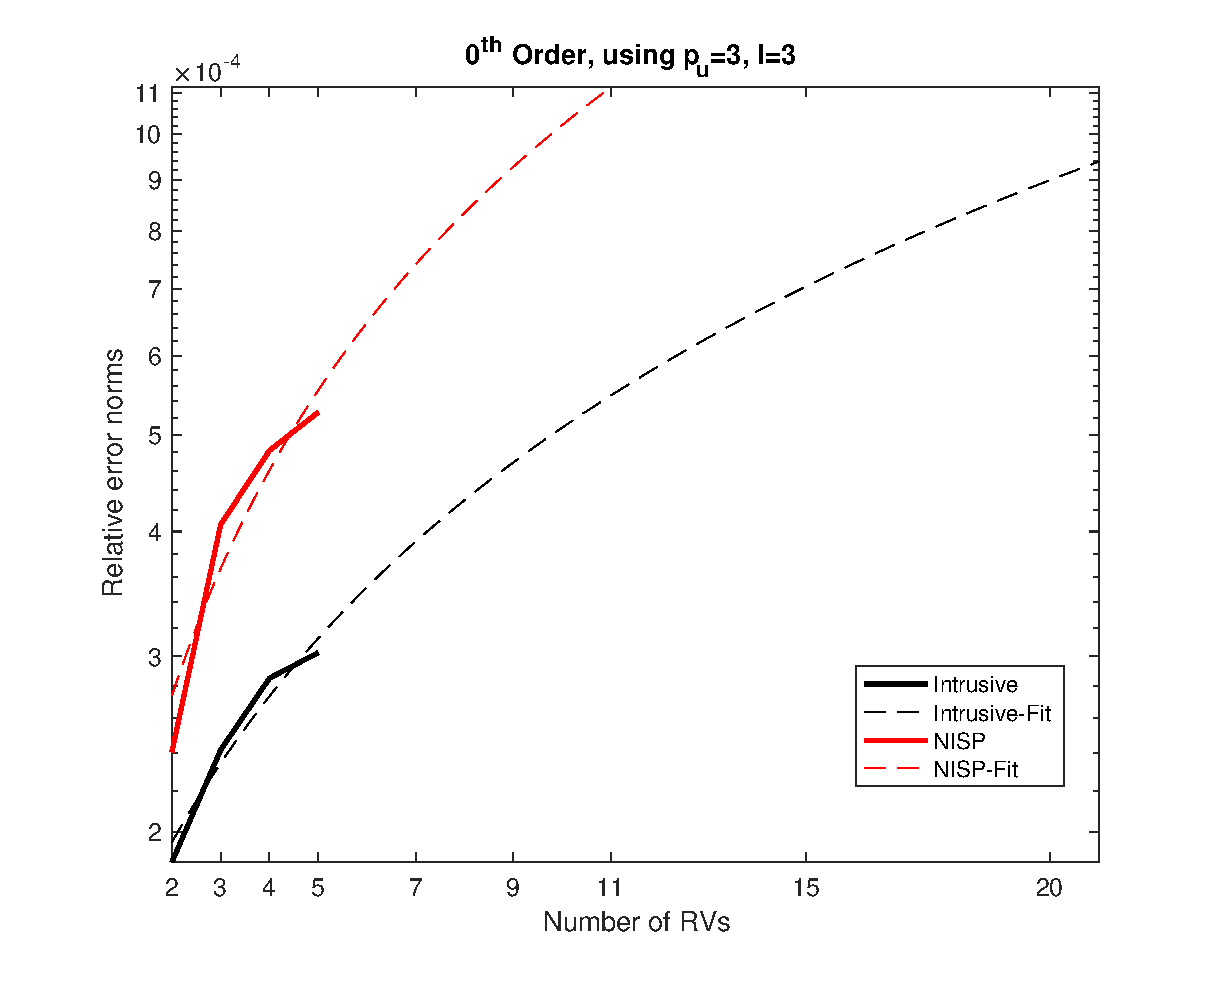
\includegraphics[width=0.6\textwidth,height=0.3\textheight]{plots/errorFits.eps}
  \caption{Extrapolated relative error convergence plots of intrusive and non-intrusive for $0^{th}$ order with third order and third level of quadrature.}
   \label{fig:Dmesh_ib}
\end{figure}

\begin{figure}[htbp]
 \centering
 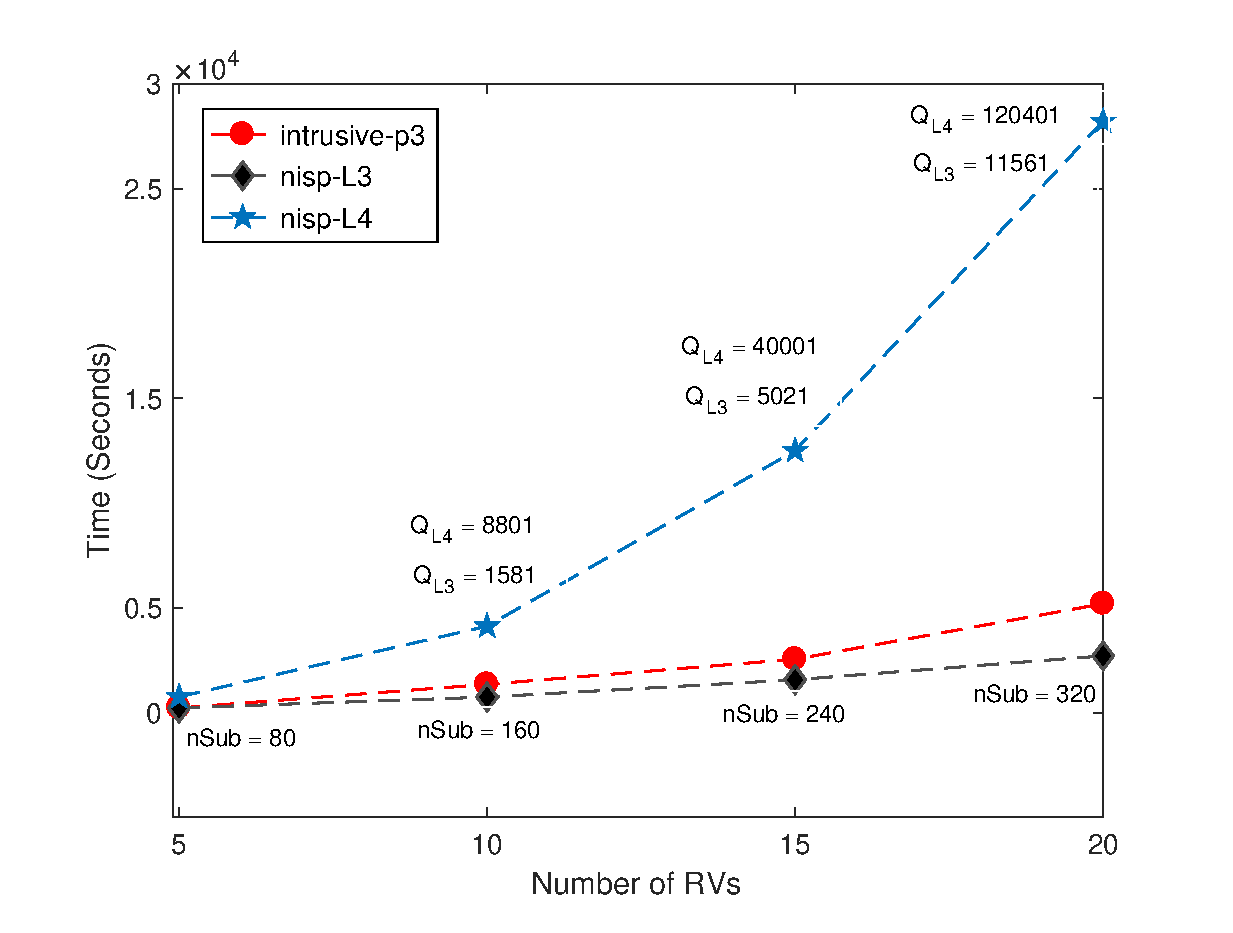
\includegraphics[width=0.7\textwidth,height=0.38\textheight]{plots/timeVnRVs_intruVnisp.eps}
 \caption{Comparison of execution time for intrusive and non-intrusive SSFEM with the fixed mesh resolution and $L = 5, 10, 15, 20$.}
 \label{fig:TimeVnRVs_intruVnisp}
\end{figure}

\

\

Computational time for the intrusive and non-intrusive SSFEM for the four different cases by selecting the number of random variables $5, 10, 15$ and $20$ is plotted in \Cref{fig:TimeVnRVs_intruVnisp}.
For the third-level sparse grid in non-intrusive approach, the total execution time for all four cases is less compared to that of intrusive approach with the third-order expansion (i.e., $l=p_{u}$). However, if we increase the level of sparse grid to $4$ (i.e., $l>p_{u})$, the computational time required to evaluate the non-intrusive samples rises quickly, especially in the cases with large number of random variables, e.g., 15 or 20.  As demonstrated earlier in~\Cref{fig:5RV}, %Fig.~1.9, %
to achieve the same level of accuracy in PCE coefficients of the solution process we need a higher-level of the sparse grid quadrature in the non-intrusive SSFEM compared to the order of expansion in the intrusive SSFEM (i.e., $l>p_{u})$.
Therefore, intrusive approach, equipped with the domain decomposition solvers shows computational advantages over non-intrusive approach for the high-dimensional, non-Gaussian stochastic input as considered in this specific application.
%This highlights the advantages of intrusive approach and demonstrate the necessity of the parallel solvers for uncertainty quantification.

% \newpage
In summary, building on the basic probabilistic formulations of BDDC/NNC~\cite{subberJCP2014} and FETI-DP~\cite{subberCMAME2013} solvers for SPDEs, this work extends the algorithms in order to tackle high-dimensional stochastic systems and perform scalability studies with respect to the number of input random variables and the corresponding PCE terms. In contrast to the references~\cite{subberCMAME2013,subberJCP2014}, direct factorization of subdomain-level matrices is avoided and better memory management strategy is implemented for high-dimensional stochastic systems. Firstly, the assembly procedure developed by the authors in~\cite{desai2019scalable,desai2017scalable}, %\Cref{alg:smap}
reduces the memory usage per core and thereby offers the ability to handle higher-dimensional stochastic systems compared to the references~\cite{subberCMAME2013,subberJCP2014}.
Moreover, the local assembly procedure provides a method to utilize existing deterministic FEM packages such as FEniCS, which drastically reduces the coding efforts required for the implementation of the DD-based intrusive SSFEM to a variety of PDEs.
Secondly, the third-level iterative solvers used to tackle the subdomain-level local systems reduce the execution time and memory consumption; and hence they offer the ability to tackle stochastic systems with larger number of input random variables and PCE terms than the previous solvers~\cite{subberCMAME2013,subberJCP2014}.
Finally, we demonstrated the computational superiority of intrusive SSFEM equipped with scalable parallel solvers over non-intrusive SSFEM for non-Gaussian and high-dimensional stochastic systems. These facts highlights the advantages of intrusive approach and demonstrate the necessity of scalable parallel solvers for extreme scale uncertainty quantification.

\section*{Acknowledgments}
The first author acknowledges  the support of  an Ontario Trillium scholarship.
The fourth author acknowledges  the support of the Canadian Department of National Defence and a Discovery Grant from Natural Sciences and Engineering Research Council of Canada.   The fifth author acknowledges the support of a  Discovery Grant from Natural Sciences and Engineering Research Council of Canada and the Canada Research Chair Program. The computing infrastructure is supported by the Canada Foundation for Innovation (CFI), the Ontario Innovation Trust (OIT),  Compute Canada and Calcul Qu\'ebec.



\clearpage

\section*{References}
\bibliographystyle{elsarticle-num}
\bibliography{references}

\end{document}
